% Options for packages loaded elsewhere
\PassOptionsToPackage{unicode}{hyperref}
\PassOptionsToPackage{hyphens}{url}
%
\documentclass[
]{book}
\usepackage{lmodern}
\usepackage{amssymb,amsmath}
\usepackage{ifxetex,ifluatex}
\ifnum 0\ifxetex 1\fi\ifluatex 1\fi=0 % if pdftex
  \usepackage[T1]{fontenc}
  \usepackage[utf8]{inputenc}
  \usepackage{textcomp} % provide euro and other symbols
\else % if luatex or xetex
  \usepackage{unicode-math}
  \defaultfontfeatures{Scale=MatchLowercase}
  \defaultfontfeatures[\rmfamily]{Ligatures=TeX,Scale=1}
\fi
% Use upquote if available, for straight quotes in verbatim environments
\IfFileExists{upquote.sty}{\usepackage{upquote}}{}
\IfFileExists{microtype.sty}{% use microtype if available
  \usepackage[]{microtype}
  \UseMicrotypeSet[protrusion]{basicmath} % disable protrusion for tt fonts
}{}
\makeatletter
\@ifundefined{KOMAClassName}{% if non-KOMA class
  \IfFileExists{parskip.sty}{%
    \usepackage{parskip}
  }{% else
    \setlength{\parindent}{0pt}
    \setlength{\parskip}{6pt plus 2pt minus 1pt}}
}{% if KOMA class
  \KOMAoptions{parskip=half}}
\makeatother
\usepackage{xcolor}
\IfFileExists{xurl.sty}{\usepackage{xurl}}{} % add URL line breaks if available
\IfFileExists{bookmark.sty}{\usepackage{bookmark}}{\usepackage{hyperref}}
\hypersetup{
  pdftitle={vignette},
  hidelinks,
  pdfcreator={LaTeX via pandoc}}
\urlstyle{same} % disable monospaced font for URLs
\usepackage{color}
\usepackage{fancyvrb}
\newcommand{\VerbBar}{|}
\newcommand{\VERB}{\Verb[commandchars=\\\{\}]}
\DefineVerbatimEnvironment{Highlighting}{Verbatim}{commandchars=\\\{\}}
% Add ',fontsize=\small' for more characters per line
\usepackage{framed}
\definecolor{shadecolor}{RGB}{248,248,248}
\newenvironment{Shaded}{\begin{snugshade}}{\end{snugshade}}
\newcommand{\AlertTok}[1]{\textcolor[rgb]{0.94,0.16,0.16}{#1}}
\newcommand{\AnnotationTok}[1]{\textcolor[rgb]{0.56,0.35,0.01}{\textbf{\textit{#1}}}}
\newcommand{\AttributeTok}[1]{\textcolor[rgb]{0.77,0.63,0.00}{#1}}
\newcommand{\BaseNTok}[1]{\textcolor[rgb]{0.00,0.00,0.81}{#1}}
\newcommand{\BuiltInTok}[1]{#1}
\newcommand{\CharTok}[1]{\textcolor[rgb]{0.31,0.60,0.02}{#1}}
\newcommand{\CommentTok}[1]{\textcolor[rgb]{0.56,0.35,0.01}{\textit{#1}}}
\newcommand{\CommentVarTok}[1]{\textcolor[rgb]{0.56,0.35,0.01}{\textbf{\textit{#1}}}}
\newcommand{\ConstantTok}[1]{\textcolor[rgb]{0.00,0.00,0.00}{#1}}
\newcommand{\ControlFlowTok}[1]{\textcolor[rgb]{0.13,0.29,0.53}{\textbf{#1}}}
\newcommand{\DataTypeTok}[1]{\textcolor[rgb]{0.13,0.29,0.53}{#1}}
\newcommand{\DecValTok}[1]{\textcolor[rgb]{0.00,0.00,0.81}{#1}}
\newcommand{\DocumentationTok}[1]{\textcolor[rgb]{0.56,0.35,0.01}{\textbf{\textit{#1}}}}
\newcommand{\ErrorTok}[1]{\textcolor[rgb]{0.64,0.00,0.00}{\textbf{#1}}}
\newcommand{\ExtensionTok}[1]{#1}
\newcommand{\FloatTok}[1]{\textcolor[rgb]{0.00,0.00,0.81}{#1}}
\newcommand{\FunctionTok}[1]{\textcolor[rgb]{0.00,0.00,0.00}{#1}}
\newcommand{\ImportTok}[1]{#1}
\newcommand{\InformationTok}[1]{\textcolor[rgb]{0.56,0.35,0.01}{\textbf{\textit{#1}}}}
\newcommand{\KeywordTok}[1]{\textcolor[rgb]{0.13,0.29,0.53}{\textbf{#1}}}
\newcommand{\NormalTok}[1]{#1}
\newcommand{\OperatorTok}[1]{\textcolor[rgb]{0.81,0.36,0.00}{\textbf{#1}}}
\newcommand{\OtherTok}[1]{\textcolor[rgb]{0.56,0.35,0.01}{#1}}
\newcommand{\PreprocessorTok}[1]{\textcolor[rgb]{0.56,0.35,0.01}{\textit{#1}}}
\newcommand{\RegionMarkerTok}[1]{#1}
\newcommand{\SpecialCharTok}[1]{\textcolor[rgb]{0.00,0.00,0.00}{#1}}
\newcommand{\SpecialStringTok}[1]{\textcolor[rgb]{0.31,0.60,0.02}{#1}}
\newcommand{\StringTok}[1]{\textcolor[rgb]{0.31,0.60,0.02}{#1}}
\newcommand{\VariableTok}[1]{\textcolor[rgb]{0.00,0.00,0.00}{#1}}
\newcommand{\VerbatimStringTok}[1]{\textcolor[rgb]{0.31,0.60,0.02}{#1}}
\newcommand{\WarningTok}[1]{\textcolor[rgb]{0.56,0.35,0.01}{\textbf{\textit{#1}}}}
\usepackage{longtable,booktabs}
% Correct order of tables after \paragraph or \subparagraph
\usepackage{etoolbox}
\makeatletter
\patchcmd\longtable{\par}{\if@noskipsec\mbox{}\fi\par}{}{}
\makeatother
% Allow footnotes in longtable head/foot
\IfFileExists{footnotehyper.sty}{\usepackage{footnotehyper}}{\usepackage{footnote}}
\makesavenoteenv{longtable}
\usepackage{graphicx,grffile}
\makeatletter
\def\maxwidth{\ifdim\Gin@nat@width>\linewidth\linewidth\else\Gin@nat@width\fi}
\def\maxheight{\ifdim\Gin@nat@height>\textheight\textheight\else\Gin@nat@height\fi}
\makeatother
% Scale images if necessary, so that they will not overflow the page
% margins by default, and it is still possible to overwrite the defaults
% using explicit options in \includegraphics[width, height, ...]{}
\setkeys{Gin}{width=\maxwidth,height=\maxheight,keepaspectratio}
% Set default figure placement to htbp
\makeatletter
\def\fps@figure{htbp}
\makeatother
\setlength{\emergencystretch}{3em} % prevent overfull lines
\providecommand{\tightlist}{%
  \setlength{\itemsep}{0pt}\setlength{\parskip}{0pt}}
\setcounter{secnumdepth}{5}
\usepackage{booktabs}
\usepackage{amsthm}
\usepackage[left=2cm,right=2cm,top=2cm,bottom=2cm]{geometry}
\makeatletter
\def\thm@space@setup{%
  \thm@preskip=8pt plus 2pt minus 4pt
  \thm@postskip=\thm@preskip
}
\makeatother
\usepackage[]{natbib}
\bibliographystyle{apalike}

\title{vignette}
\author{}
\date{\vspace{-2.5em}}

\begin{document}
\maketitle

{
\setcounter{tocdepth}{1}
\tableofcontents
}
\hypertarget{status}{%
\chapter{Status}\label{status}}

This status report outlines the code we are developing to process \texttt{WinCruz} data and prepare it for density estimation analysis using \texttt{distance} and related packages in \texttt{R}.

\hypertarget{recent-changes}{%
\subsection*{Recent changes}\label{recent-changes}}
\addcontentsline{toc}{subsection}{Recent changes}

\hypertarget{week-of-jan.-2}{%
\subsubsection*{Week of Jan.~2}\label{week-of-jan.-2}}
\addcontentsline{toc}{subsubsection}{Week of Jan.~2}

\begin{itemize}
\item
  Refinement of cruise summarization functions (see Chapter 6).
\item
  Addition of interactive map (see \texttt{LTabundR::cruz\_map()} documentation).
\item
  Addition of interactive data explorer \texttt{Shiny} app (see \texttt{LTabundR::cruz\_explorer()} documentation, with examples in \texttt{LTabundR-dev/test\_code/CNP/data\_processing.R}).
\end{itemize}

\hypertarget{week-of-dec.-26}{%
\subsubsection*{Week of Dec.~26}\label{week-of-dec.-26}}
\addcontentsline{toc}{subsubsection}{Week of Dec.~26}

\begin{itemize}
\item
  Completion of comparison and reconciliation between \texttt{ABUND} and \texttt{LTabundR}, involving various minor debugs. See details \href{https://docs.google.com/presentation/d/1Vv0Yb2_gk0cEC1OlXlm6ffL9ug99bYvkpLkczg6pb2Q/edit?usp=sharing}{here}.
\item
  Completion of package and function documentation (to date).
\end{itemize}

\hypertarget{week-of-dec.-21}{%
\subsubsection*{Week of Dec.~21}\label{week-of-dec.-21}}
\addcontentsline{toc}{subsubsection}{Week of Dec.~21}

\begin{itemize}
\item
  Refined code for \protect\hyperlink{subgroups}{subgroup-level school size estimation}. This feature is now stable.
\item
  Next item.
\end{itemize}

\hypertarget{week-of-dec.-13}{%
\subsubsection*{Week of Dec.~13}\label{week-of-dec.-13}}
\addcontentsline{toc}{subsubsection}{Week of Dec.~13}

\begin{itemize}
\item
  Development of features for handling subgroup-level analysis of false killer whale sightings. (more soon).
\item
  A wide variety of minor improvements as part of a major push to compare \texttt{LTabundR} results to those from \texttt{ABUND7} and \texttt{ABUND9}. This included an effort to articulate the differences between \texttt{LTabundR} and \texttt{ABUND} routines (detailed in a \protect\hyperlink{abund9_compare}{new appendix}), and to quantify the correspondence (or lack thereof) between the two programs. This involved the development of a function, \texttt{abund9\_compare()}, which is not featured in this vignette but can be used to compare \texttt{LTabundR} outputs with those from \texttt{ABUND9}. We are also documenting comparisons on \href{https://docs.google.com/document/d/1_EZqzOnwSZZCitqTJFIbznGy2Njwbj1YOqMQcbcHI7k/edit?usp=sharing}{this document}.
\item
  Made \texttt{beaufort\_range} as a cohort-specific setting, instead of a survey-wide setting.
\end{itemize}

\hypertarget{prior-to-week-of-dec.-8}{%
\subsubsection*{Prior to week of Dec.~8}\label{prior-to-week-of-dec.-8}}
\addcontentsline{toc}{subsubsection}{Prior to week of Dec.~8}

\begin{itemize}
\item
  Added a new survey-wide setting, \texttt{out\_handling}, that determines how data occurring outside of geographic strata will be handled. Currently the two options are \texttt{"remove"} (the default), which removes data occurring outside of the strata (speeds things up, reduces memory needs), and \texttt{"stratum"}, which assigns all exterior events to an \texttt{"out"} stratum.
\item
  Modified \texttt{segmentize()} function so that a list of segments is not returned to the user; that feature was created enormous objects (\textgreater{} 1 GB for the 1986 - 2020 CNP DAS data) and is not useful enough to retain as a standing slot. A list like that can be easily produced using a \texttt{dplyr} pipe (\texttt{group\_by(seg\_id)\ \%\textgreater{}\%\ group\_split()}) when the need arises (e.g., in \texttt{map\_effort()} -- this function has also been updated to accommodate this new change).
\item
  Fixed minutiae regarding group size estimation: sightings with missing data are given a school size estimate of 1, as done in \texttt{ABUND}; geometric mean functions have been fixed.
\item
  Added progress indicator to \texttt{process\_sightings()}.
\item
  New \texttt{format\_distance()} function creates tables that match \texttt{EFFORT.csv} and \texttt{SIGHTINGS.csv}. (See \protect\hyperlink{df}{here}.)
\item
  New \texttt{process\_surveys()} function provides a wrapper for all data processing functions in a single command. This will be the main function that researchers use to process their data. All other functions are called \emph{within} this function, and will rarely be called directly by researchers except in special analyses. This is explained at the top of the page on \protect\hyperlink{processing}{Data Processing}. This function includes an option for saving the result locally as a \texttt{RData} file, which allows the user to run this function once and save the result for later sessions.
\item
  New helper function, \texttt{read\_polygon()}, reads a \texttt{DAT} file of polygon coordinates and converts it to a dataframe compatible with \texttt{LTabundR} functions. Can handle files with multiple polygons.
\item
  Skeletonized new summary functions (see the \protect\hyperlink{summarize}{Summarize page}).
\item
  Ship name is now added to all dataframes.
\item
  New \texttt{process\_sightings()} function, with code for calibrating group sizes according to user-provided coefficient tables (mirroring \texttt{ABUND9} with slight mods, e.g., school size threshold for observers not in the \texttt{Coeff.DAT} file.). (Details: the function \texttt{process\_sightings()} relies upon a utility function, \texttt{group\_size()}, which in turn relies upon \texttt{group\_size\_calibrate()}.)
\item
  Added cohort-specific setting, \texttt{school\_size\_calibrate}, that allows researchers to specify whether a cohort should or should not have school sizes calibrated. Example use case: \texttt{school\_size\_calibrate\ =\ TRUE} for a cohort of dolphin species, but make it \texttt{FALSE} for a cohort of large baleen whales.
\item
  Basic function for mapping sightings (QA/QC): \texttt{map\_sightings()}.
\item
  Added detail/polish to vignette pages on \protect\hyperlink{settings}{Settings}, \protect\hyperlink{processing}{Processing Data}, and the \protect\hyperlink{segmentizing}{Appendix on Segmentizing}. I believe these are ready for close review.
\item
  Added detailed comments to code for all functions to date.
\end{itemize}

\hypertarget{next-focus}{%
\subsection*{Next focus}\label{next-focus}}
\addcontentsline{toc}{subsection}{Next focus}

\begin{itemize}
\tightlist
\item
  Data evaluation and big picture planning of detection function and parameter estimation.
\end{itemize}

\hypertarget{questions-for-amanda}{%
\subsection*{Questions for Amanda}\label{questions-for-amanda}}
\addcontentsline{toc}{subsection}{Questions for Amanda}

\hypertarget{questions-for-jay}{%
\subsection*{Questions for Jay}\label{questions-for-jay}}
\addcontentsline{toc}{subsection}{Questions for Jay}

\begin{itemize}
\tightlist
\item
  How does ABUND protect against long gaps between DAS rows in its distance-traveled calculations? From what I can tell in the FORTRAN code, it seems possible for long gaps to be mistaken for effort.
\end{itemize}

\hypertarget{part-tutorial}{%
\part{Tutorial}\label{part-tutorial}}

\hypertarget{install}{%
\chapter{\texorpdfstring{Install \texttt{LTabundR}}{Install LTabundR}}\label{install}}

\hypertarget{option-1-install-from-github}{%
\section*{Option 1: Install from GitHub}\label{option-1-install-from-github}}
\addcontentsline{toc}{section}{Option 1: Install from GitHub}

Since the package is currently private, this is more complicated than it will be once the package is released.

The first step is creating an \texttt{R} environment variable containing your \texttt{GitHub} personal access token.

Complete these instructions \textbf{only once:}

\begin{Shaded}
\begin{Highlighting}[]
\CommentTok{# Open your .Renviron file}
\KeywordTok{library}\NormalTok{(usethis)}
\NormalTok{usethis}\OperatorTok{::}\KeywordTok{edit_r_environ}\NormalTok{()}

\CommentTok{# Add your GitHub personal access token as a variable in `.Renviron`}
\NormalTok{GITHUB_TOKEN =}\StringTok{ 'your_token_goes_here_as_a_character_string'}

\CommentTok{# Save and close your .Renviron file}
\CommentTok{# Reload .Renviron}
\KeywordTok{readRenviron}\NormalTok{(}\StringTok{'~/.Renviron'}\NormalTok{)}
\end{Highlighting}
\end{Shaded}

Then run this code \textbf{every time} you want to reinstall / update the package:

\begin{Shaded}
\begin{Highlighting}[]
\KeywordTok{library}\NormalTok{(devtools)}
\NormalTok{github_token <-}\StringTok{ }\KeywordTok{Sys.getenv}\NormalTok{(}\StringTok{"GITHUB_TOKEN"}\NormalTok{)}
\NormalTok{devtools}\OperatorTok{::}\KeywordTok{install_github}\NormalTok{(}\DataTypeTok{repo =} \StringTok{'amandalbradford/LTabundR-dev'}\NormalTok{,}
                         \DataTypeTok{subdir=}\StringTok{'LTabundR'}\NormalTok{,}
                         \DataTypeTok{auth_token=}\NormalTok{github_token,}
                         \DataTypeTok{force=}\OtherTok{TRUE}\NormalTok{)}
\KeywordTok{library}\NormalTok{(LTabundR)}
\end{Highlighting}
\end{Shaded}

\hypertarget{option-2-install-locally}{%
\section*{Option 2: Install locally}\label{option-2-install-locally}}
\addcontentsline{toc}{section}{Option 2: Install locally}

For now you can also install or update the package locally, using this code:

\begin{Shaded}
\begin{Highlighting}[]
\KeywordTok{library}\NormalTok{(devtools) }

\CommentTok{# Remove the package, if you have an earlier version of it on your machine}
\ControlFlowTok{if}\NormalTok{(}\StringTok{'LTAabundR'} \OperatorTok\StringTok{ }\KeywordTok{installed.packages}\NormalTok{())\{}\KeywordTok{remove.packages}\NormalTok{(}\StringTok{'LTabundR'}\NormalTok{)\} }

\CommentTok{# Specify the path to the package's project folder.}
\NormalTok{path_to_package <-}\StringTok{ '../LTabundR-dev/LTabundR'}

\CommentTok{# Update function documentation}
\KeywordTok{document}\NormalTok{(path_to_package) }

\CommentTok{# Install package and any dependencies you need}
\KeywordTok{install}\NormalTok{(path_to_package) }

\KeywordTok{library}\NormalTok{(LTabundR)}
\end{Highlighting}
\end{Shaded}

\hypertarget{settings}{%
\chapter{Settings}\label{settings}}

To customize the way data are processed and included in your analysis, use the \texttt{load\_settings()} function. This function emulates and expands upon the settings file, \texttt{ABUND.INP}, that was used to run \texttt{ABUND7/9} in \texttt{FORTRAN}.

This function allows you to use `factory defaults' if you don't wish to specify anything special such as strata or study area polygons:

\begin{Shaded}
\begin{Highlighting}[]
\NormalTok{settings <-}\StringTok{ }\KeywordTok{load_settings}\NormalTok{()}
\end{Highlighting}
\end{Shaded}

If you do not want to use all the defaults, you can give \texttt{load\_settings()} some custom inputs. The function accepts four arguments:

\begin{itemize}
\item
  \texttt{strata}: dataframe(s) of coordinates
\item
  \texttt{study\_area}: a dataframe of coordinates
\item
  \texttt{survey}: settings that will apply universally to the analysis
\item
  \texttt{cohorts}: settings that are specific to groups of species. By providing cohort-specific settings, the code for a single analysis becomes fully flexible to prepare and more easily reproduced, since the code only needs to be run once without modification.
\end{itemize}

The output of \texttt{load\_settings()} is a named list with a slot for each of these arguments:

\begin{Shaded}
\begin{Highlighting}[]
\NormalTok{settings }\OperatorTok\StringTok{ }\NormalTok{names}
\NormalTok{[}\DecValTok{1}\NormalTok{] }\StringTok{"strata"}     \StringTok{"study_area"} \StringTok{"survey"}     \StringTok{"cohorts"}   
\end{Highlighting}
\end{Shaded}

\hypertarget{survey-strata}{%
\section*{Survey strata}\label{survey-strata}}
\addcontentsline{toc}{section}{Survey strata}

Stratum polygons can be provided as a named list of \texttt{data.frame} objects. Each \texttt{data.frame} must have \texttt{Lat} and \texttt{Lon} as the first two columns, providing coordinates in decimal degrees in which South and West coordinates are negative. Other columns are allowed, but the first two need to be \texttt{Lon} and \texttt{Lat}. The name of the slot holding the \texttt{data.frame} will be used as a reference name for the stratum.

If \texttt{strata} is \texttt{NULL}, abundance will not be estimated; only density within the searched area (i.e., the total segment length x effective strip width).

While users are welcome to upload polygons of their own, the package comes with ``stock'' polygons for strata that are commonly used in the main NMFS study regions: the Central North Pacific (CNP, including Hawaii) \ldots{}

\begin{Shaded}
\begin{Highlighting}[]
\KeywordTok{data}\NormalTok{(strata_cnp) }
\KeywordTok{names}\NormalTok{(strata_cnp)}
\NormalTok{[}\DecValTok{1}\NormalTok{] }\StringTok{"HI_EEZ"}   \StringTok{"WHICEAS"}  \StringTok{"OtherCNP"}
\end{Highlighting}
\end{Shaded}

\ldots the California Current System (CCS) \ldots{}

\begin{Shaded}
\begin{Highlighting}[]
\KeywordTok{data}\NormalTok{(strata_ccs) }
\KeywordTok{names}\NormalTok{(strata_ccs)}
\NormalTok{[}\DecValTok{1}\NormalTok{] }\StringTok{"CCS"}         \StringTok{"Southern_CA"} \StringTok{"Central_CA"}  \StringTok{"Nothern_CA"}  \StringTok{"OR_WA"}      
\end{Highlighting}
\end{Shaded}

\ldots{} and the Eastern Tropical Pacific (ETP):

\begin{Shaded}
\begin{Highlighting}[]
\KeywordTok{data}\NormalTok{(strata_etp) }
\KeywordTok{names}\NormalTok{(strata_etp)}
\NormalTok{ [}\DecValTok{1}\NormalTok{] }\StringTok{"MOPS_AreaCoreM"}     \StringTok{"MOPS_AreaIn"}        \StringTok{"MOPS_AreaIn1"}      
\NormalTok{ [}\DecValTok{4}\NormalTok{] }\StringTok{"MOPS_AreaIn2"}       \StringTok{"MOPS_AREAINS"}       \StringTok{"MOPS_AREAMID"}      
\NormalTok{ [}\DecValTok{7}\NormalTok{] }\StringTok{"MOPS_AreaMid1"}      \StringTok{"MOPS_AreaMid2"}      \StringTok{"MOPS_AreaMOPS"}     
\NormalTok{[}\DecValTok{10}\NormalTok{] }\StringTok{"MOPS_AREANORS"}      \StringTok{"MOPS_AreaOuterM"}    \StringTok{"MOPS_AreaSou"}      
\NormalTok{[}\DecValTok{13}\NormalTok{] }\StringTok{"MOPS_AREASOUS"}      \StringTok{"MOPS_AreaSpin"}      \StringTok{"MOPS_AreaSpinS"}    
\NormalTok{[}\DecValTok{16}\NormalTok{] }\StringTok{"MOPS_AREAWES"}       \StringTok{"PODS_93STRAT1"}      \StringTok{"PODS_93STRAT2"}     
\NormalTok{[}\DecValTok{19}\NormalTok{] }\StringTok{"PODS_Area92"}        \StringTok{"PODS_AREA92RS"}      \StringTok{"PODS_Area92s"}      
\NormalTok{[}\DecValTok{22}\NormalTok{] }\StringTok{"PODS_AREA93"}        \StringTok{"PODS_AREA93A"}       \StringTok{"PODS_AREA93AR"}     
\NormalTok{[}\DecValTok{25}\NormalTok{] }\StringTok{"PODS_AREA93AS"}      \StringTok{"PODS_AREA93BR"}      \StringTok{"PODS_AREA93M"}      
\NormalTok{[}\DecValTok{28}\NormalTok{] }\StringTok{"PODS_AREA93MS"}      \StringTok{"PODS_AREA93R"}       \StringTok{"PODS_AREA93R1"}     
\NormalTok{[}\DecValTok{31}\NormalTok{] }\StringTok{"PODS_AREA93R2"}      \StringTok{"PODS_AREA93RS"}      \StringTok{"PODS_AREA93S"}      
\NormalTok{[}\DecValTok{34}\NormalTok{] }\StringTok{"PODS_AREANCOR"}      \StringTok{"PODS_GOCpoly"}       \StringTok{"Pre1986_Area79ES1"} 
\NormalTok{[}\DecValTok{37}\NormalTok{] }\StringTok{"Pre1986_Area79ES1s"} \StringTok{"Pre1986_Area79ES2"}  \StringTok{"Pre1986_Area79ES2s"}
\NormalTok{[}\DecValTok{40}\NormalTok{] }\StringTok{"Pre1986_Area79NE1"}  \StringTok{"Pre1986_Area79NE1s"} \StringTok{"Pre1986_Area79NE2"} 
\NormalTok{[}\DecValTok{43}\NormalTok{] }\StringTok{"Pre1986_Area79NE2s"} \StringTok{"Pre1986_Area79NE3"}  \StringTok{"Pre1986_Area79NE3s"}
\NormalTok{[}\DecValTok{46}\NormalTok{] }\StringTok{"Pre1986_AreaCal"}    \StringTok{"Pre1986_AreaCals"}   \StringTok{"Pre1986_AreaMid"}   
\NormalTok{[}\DecValTok{49}\NormalTok{] }\StringTok{"Pre1986_AreaMidS"}   \StringTok{"Pre1986_AreaNorth"}  \StringTok{"Pre1986_AreaNorthS"}
\NormalTok{[}\DecValTok{52}\NormalTok{] }\StringTok{"Pre1986_AreaSouth"}  \StringTok{"Pre1986_AreaSouthS"} \StringTok{"STAR_Area98a"}      
\NormalTok{[}\DecValTok{55}\NormalTok{] }\StringTok{"STAR_Area98b"}       \StringTok{"STAR_AreaCore"}      \StringTok{"STAR_AreaCore2"}    
\NormalTok{[}\DecValTok{58}\NormalTok{] }\StringTok{"STAR_AreaCoreS"}     \StringTok{"STAR_AreaNCoast"}    \StringTok{"STAR_AreaNCstS"}    
\NormalTok{[}\DecValTok{61}\NormalTok{] }\StringTok{"STAR_AreaOuter"}     \StringTok{"STAR_AreaOuter00"}   \StringTok{"STAR_AreaSCoast"}   
\NormalTok{[}\DecValTok{64}\NormalTok{] }\StringTok{"STAR_AreaSCstS"}     \StringTok{"STAR_AreaSPn"}       \StringTok{"STAR_AreaSPs"}      
\NormalTok{[}\DecValTok{67}\NormalTok{] }\StringTok{"STAR_AreaSTAR"}      \StringTok{"STAR_AreaSTAR2"}     \StringTok{"STAR_AreaSTARlite"} 
\NormalTok{[}\DecValTok{70}\NormalTok{] }\StringTok{"STAR_Dcaparea"}     
\end{Highlighting}
\end{Shaded}

The package includes functions for visualizing and selecting from these strata. See the \protect\hyperlink{stratagallery}{Strata Gallery} appendix.

\hypertarget{study-area-polygon}{%
\section*{Study area polygon}\label{study-area-polygon}}
\addcontentsline{toc}{section}{Study area polygon}

The \texttt{study\_area} argument accepts a single \texttt{data.frame}, formatted the same as those for the \texttt{strata} argument, or a numeric value indicating the area of your study area in square km. If \texttt{study\_area} is \texttt{NULL}, abundance will not be estimated; only density.

Study area polygons can be provided in the same format as strata: a two-column \texttt{csv} (column names \texttt{Lon} and \texttt{Lat} with decimal-degree coordinates).

A stock study area polygon is available for the CNP:

\begin{Shaded}
\begin{Highlighting}[]
\KeywordTok{data}\NormalTok{(study_cnp) }
\NormalTok{study_cnp}
\NormalTok{   Lon   Lat}
\DecValTok{1} \DecValTok{-131} \FloatTok{40.00}
\DecValTok{2} \DecValTok{-126} \FloatTok{32.05}
\DecValTok{3} \DecValTok{-120} \FloatTok{25.00}
\DecValTok{4} \DecValTok{-120} \FloatTok{-5.00}
\DecValTok{5} \DecValTok{-185} \FloatTok{-5.00}
\DecValTok{6} \DecValTok{-185} \FloatTok{40.00}
\DecValTok{7} \DecValTok{-131} \FloatTok{40.00}
\end{Highlighting}
\end{Shaded}

\hypertarget{survey-wide-settings}{%
\section*{Survey-wide settings}\label{survey-wide-settings}}
\addcontentsline{toc}{section}{Survey-wide settings}

Survey-wide settings apply universally to all species in the analysis.

\hypertarget{defaults}{%
\subsection*{Defaults}\label{defaults}}
\addcontentsline{toc}{subsection}{Defaults}

\begin{Shaded}
\begin{Highlighting}[]
\NormalTok{settings}\OperatorTok{$}\NormalTok{survey}
\OperatorTok{$}\NormalTok{out_handling}
\NormalTok{[}\DecValTok{1}\NormalTok{] }\StringTok{"remove"}  \StringTok{"stratum"}

\OperatorTok{$}\NormalTok{max_row_interval}
\NormalTok{[}\DecValTok{1}\NormalTok{] }\DecValTok{360}

\OperatorTok{$}\NormalTok{segment_method}
\NormalTok{[}\DecValTok{1}\NormalTok{] }\StringTok{"day"}

\OperatorTok{$}\NormalTok{segment_target_km}
\NormalTok{[}\DecValTok{1}\NormalTok{] }\DecValTok{150}

\OperatorTok{$}\NormalTok{segment_max_interval}
\NormalTok{[}\DecValTok{1}\NormalTok{] }\DecValTok{48}

\OperatorTok{$}\NormalTok{segment_type_handling}
\NormalTok{[}\DecValTok{1}\NormalTok{] }\StringTok{"separate"} \StringTok{"pool"}    

\OperatorTok{$}\NormalTok{segment_remainder_handling}
\NormalTok{[}\DecValTok{1}\NormalTok{] }\StringTok{"append"}  \StringTok{"segment"}

\OperatorTok{$}\NormalTok{ship_list}
\OtherTok{NULL}

\OperatorTok{$}\NormalTok{species_codes}
\OtherTok{NULL}

\OperatorTok{$}\NormalTok{group_size_coefficients}
\OtherTok{NULL}

\OperatorTok{$}\NormalTok{smear_angles}
\NormalTok{[}\DecValTok{1}\NormalTok{] }\OtherTok{FALSE}

\OperatorTok{$}\NormalTok{random_seed}
\NormalTok{[}\DecValTok{1}\NormalTok{] }\DecValTok{833171}

\OperatorTok{$}\NormalTok{verbose}
\NormalTok{[}\DecValTok{1}\NormalTok{] }\OtherTok{TRUE}
\end{Highlighting}
\end{Shaded}

Defaults for the \texttt{survey} argument list are built up efficiently using the function \texttt{load\_survey\_settings()} (see example code at bottom).

\hypertarget{details}{%
\subsection*{Details}\label{details}}
\addcontentsline{toc}{subsection}{Details}

The \texttt{survey\_settings} input accepts a list with any of the following named slots.

\begin{itemize}
\item
  \textbf{\texttt{out\_handling:}} the first slot allows you to specify how data occurring outside of geo-strata should be handled. If this is set to \texttt{"remove"}, those rows will be filtered out of the data early in the process. This reduces memory usage, speeds up processing, and gives you geographic control of how effort and sightings will be summarize. If this is set to \texttt{"stratum"}, those data will be assigned to a fake geo-stratum, named \texttt{"out"}. Effort in the \texttt{"out"} stratum will not be segmentized, but \texttt{"out"} sightings will be processed and retained in the final datasets. This setting might be useful if you want to use \texttt{"out"} data for survey summaries and/or detection function estimation. The default is \texttt{"remove"}, since that saves the most time and memory.
\item
  \textbf{\texttt{segment\_method:}} This and the next few slots are devoted to controlling how effort will be ``segmentized'', or chopped into discrete sections for the purposes of estimating the variabce of the abundance estimate. The two method options are \texttt{"day"} -- all effort within the same Cruise-StudyArea-Stratum-Year-Effort scenario will be binned into segments by calendar date -- and \texttt{"equallength"} -- effort within each unique effort scenario (Cruise-StudyArea-etc.) will be divided into segments of approximately equal length. See the \protect\hyperlink{segmentizing}{Appendix on segmentizing} for details.
\item
  \textbf{\texttt{segment\_target\_km:}} if segmenting by \texttt{"equallength"}, this field allows you to specify what that target length is, in km.
\item
  \textbf{\texttt{segment\_max\_km\_gap:}} the segmentizing function works by calculating the distance between each row of \texttt{DAS} data. If that distance exceeds the length specified here (e.g., 5 km), the function will assume that there was a break in effort.
\item
  \textbf{\texttt{segment\_max\_interval:}} if segmentizing by \texttt{"equallength"}, this setting allows you to specify the time gaps in effort that are allowed to be contained within a single segment. For example, if your goal is a few large segments of equal length (e.g., 150-km segments, for bootstrap estimation of density variance), you are probably willing for discrete periods of effort to be concatenated into a single segment, even if the gaps between effort are as large as 1 or 2 days, in which case you would set \texttt{segment\_max\_interval} to 24 or 48 (hours), respectively. However, if your goal is many smaller segments (e.g., 5-km segments, for habitat modeling), you want to ensure that effort is contiguous so that segment locations can be accurately related to environmental variables, in which case you would set \texttt{segment\_max\_interval} to be very small (e.g., .2 hours, or 12 minutes). Setting this interval to a small number, such as 0.2, also allows the segmentizing function overlook momentary breaks in effort, such as when an unofficial observer logs a sighting.
\item
  \textbf{\texttt{segment\_type\_handling:}} if \texttt{"pool"}, all effort types that qualify as valid according to \texttt{cohort\_settings} (see next section) will be pooled together, making it possible for different effort types to occur in the same segment. Specifically, when this setting is \texttt{"pool"}, the \texttt{EffType}'s ``\texttt{S}'' and ``\texttt{F}'' are allowed to occur in the same segment; if this argument is \texttt{"separate"}, segments will only be allowed to contain a single effort type.
\item
  \textbf{\texttt{segment\_remainder\_handling:}} if segmentizing by \texttt{"equallength"}, periods of effectively-contiguous effort (as specified by \texttt{segment\_max\_interval}) are unlikely to be perfectly divisible by your \texttt{segment\_target\_km}; there is going to be a remainder. You can handle this remainder in three ways: (1) \texttt{"disperse"} allows the function to adjust \texttt{segment\_target\_km} so that there is in fact no remainder, effectively dispersing the remainder evenly across all segments within that period of contiguous effort; (2) \texttt{"append"} asks the function to append the remainder to a randomly selected segment, such that most segments are the target length with the exception of one longer one; or (3) \texttt{"segment"} asks the function to simply place the remainder in its own segment, placed randomly within the period of contiguous effort. This setting also has a second layer of versatility, because it can accept a one- or two-element character vector. If a two-element vector is provided (e.g., \texttt{c("append","segment")}), the first element will be used in the event that the remainder is less than or equal to half your \texttt{segment\_target\_km}; if the remainder is more than half that target length, the second element will be used. This feature allows for replication of the segmentizing methods in \href{https://www.int-res.com/abstracts/meps/v413/p163-183/}{Becker et al.~(2010)}.
\end{itemize}

The remaining slots in \texttt{survey\_settings} pertain to various datasets and settings used in data processing:

\begin{itemize}
\item
  \textbf{\texttt{ship\_list:}} A \texttt{data.frame} containing a list of ship names. If not provided the default version, which was current as of the release of \texttt{ABUND9} in 2020, will be used (\texttt{data(ships)}). Supplied \texttt{data.frames} must match the column naming structure of \texttt{data(ships)}.
\item
  \textbf{\texttt{species\_codes:}} A \texttt{data.frame} containing species codes. If not provided the default version, which was current as of the release of \texttt{ABUND9} in 2020, will be used (\texttt{data(species\_codes)}). Supplied \texttt{data.frames} must match the column naming structure of \texttt{data(species\_codes)}.
\item
  \textbf{\texttt{group\_size\_coefficients:}} A \texttt{data.frame} of calibration factors. Find details in the subsection on processing sightings and \protect\hyperlink{ss_calibration}{estimating school size}.
\item
  \textbf{\texttt{smear\_angles:}} If \texttt{TRUE} (the default is \texttt{FALSE}), bearing angles to a group of animals will be ``smeared'' by adding a uniformly distributed random number between -5 and +5 degrees. This has not been used in any recent analyses because observers have not been rounding angles as much as they used to. It was suggested by Buckland as a method for dealing with rounding which is especially influential when rounding to zero places many sightings at zero perpendicular distance.
\item
  \textbf{\texttt{random\_seed:}} a number used as the seed for stages involving random number generation. If not \texttt{NULL}, the results will be exactly reproducible. Default is \texttt{833171} (\emph{sensu} example code in \texttt{ABUND9}).
\item
  \textbf{\texttt{verbose:}} If \texttt{TRUE} (the default), status updates will be printed to the \texttt{R} console.
\end{itemize}

\hypertarget{cohort-specific-settings}{%
\section*{Cohort-specific settings}\label{cohort-specific-settings}}
\addcontentsline{toc}{section}{Cohort-specific settings}

Cohort-specific settings apply only to a group of species. Since you can add as many cohorts to a \texttt{settings} object as you need, this allows you to stage your entire analysis and run your code once, without modifying code between the analysis of each cohort.

\hypertarget{defaults-1}{%
\subsection*{Defaults}\label{defaults-1}}
\addcontentsline{toc}{subsection}{Defaults}

The default is to use a single cohort for all species:

\begin{Shaded}
\begin{Highlighting}[]
\NormalTok{settings}\OperatorTok{$}\NormalTok{cohorts }\OperatorTok\StringTok{ }\NormalTok{names}
\NormalTok{[}\DecValTok{1}\NormalTok{] }\StringTok{"default"}
\end{Highlighting}
\end{Shaded}

Default values for the \texttt{default} cohort:

\begin{Shaded}
\begin{Highlighting}[]
\NormalTok{settings}\OperatorTok{$}\NormalTok{cohorts}\OperatorTok{$}\NormalTok{default}
\OperatorTok{$}\NormalTok{id}
\NormalTok{[}\DecValTok{1}\NormalTok{] }\StringTok{"default"}

\OperatorTok{$}\NormalTok{species}
\OtherTok{NULL}

\OperatorTok{$}\NormalTok{probable_species}
\NormalTok{[}\DecValTok{1}\NormalTok{] }\OtherTok{FALSE}

\OperatorTok{$}\NormalTok{sighting_method}
\NormalTok{[}\DecValTok{1}\NormalTok{] }\DecValTok{0}

\OperatorTok{$}\NormalTok{cue_range}
\NormalTok{[}\DecValTok{1}\NormalTok{] }\DecValTok{0} \DecValTok{1} \DecValTok{2} \DecValTok{3} \DecValTok{4} \DecValTok{5} \DecValTok{6} \DecValTok{7}

\OperatorTok{$}\NormalTok{school_size_range}
\NormalTok{[}\DecValTok{1}\NormalTok{]     }\DecValTok{0} \DecValTok{10000}

\OperatorTok{$}\NormalTok{school_size_calibrate}
\NormalTok{[}\DecValTok{1}\NormalTok{] }\OtherTok{TRUE}

\OperatorTok{$}\NormalTok{calibration_floor}
\NormalTok{[}\DecValTok{1}\NormalTok{] }\DecValTok{0}

\OperatorTok{$}\NormalTok{use_low_if_na}
\NormalTok{[}\DecValTok{1}\NormalTok{] }\OtherTok{FALSE}

\OperatorTok{$}\NormalTok{io_sightings}
\NormalTok{[}\DecValTok{1}\NormalTok{] }\DecValTok{0}

\OperatorTok{$}\NormalTok{geometric_mean_group}
\NormalTok{[}\DecValTok{1}\NormalTok{] }\OtherTok{TRUE}

\OperatorTok{$}\NormalTok{truncation_km}
\NormalTok{[}\DecValTok{1}\NormalTok{] }\FloatTok{5.5}

\OperatorTok{$}\NormalTok{beaufort_range}
\NormalTok{[}\DecValTok{1}\NormalTok{] }\DecValTok{0} \DecValTok{1} \DecValTok{2} \DecValTok{3} \DecValTok{4} \DecValTok{5} \DecValTok{6}

\OperatorTok{$}\NormalTok{abeam_sightings}
\NormalTok{[}\DecValTok{1}\NormalTok{] }\OtherTok{FALSE}

\OperatorTok{$}\NormalTok{strata_overlap_handling}
\NormalTok{[}\DecValTok{1}\NormalTok{] }\StringTok{"smallest"} \StringTok{"largest"}  \StringTok{"each"}    

\OperatorTok{$}\NormalTok{density_types}
\NormalTok{[}\DecValTok{1}\NormalTok{] }\StringTok{"S"} \StringTok{"F"}

\OperatorTok{$}\NormalTok{density_modes}
\NormalTok{[}\DecValTok{1}\NormalTok{] }\StringTok{"P"} \StringTok{"C"}

\OperatorTok{$}\NormalTok{density_on_off}
\NormalTok{[}\DecValTok{1}\NormalTok{] }\OtherTok{TRUE}

\OperatorTok{$}\NormalTok{distance_types}
\OtherTok{NULL}

\OperatorTok{$}\NormalTok{distance_modes}
\OtherTok{NULL}

\OperatorTok{$}\NormalTok{distance_on_off}
\OtherTok{NULL}
\end{Highlighting}
\end{Shaded}

Defaults for the \texttt{cohorts} argument list is built up efficiently using the function \texttt{load\_cohort\_settings()} (see example code at bottom).

\hypertarget{details-1}{%
\subsection*{Details}\label{details-1}}
\addcontentsline{toc}{subsection}{Details}

The \texttt{cohort\_settings} input accepts a list of any length. Each slot in that list can contain settings for a different cohort. Each cohort list can have any of the following named slots:

\begin{itemize}
\item
  \textbf{\texttt{id:}} An informal identifier for this cohort, to help you keep track of which cohort is which. For example, settings for a cohort of large whales species could be named \texttt{"big\ whales"}; settings for small delphinids and phocoenids could be named \texttt{"small\_odontocetes"}; settings for beaked whales could be named \texttt{"beakers"}.
\item
  \textbf{\texttt{species:}} A character vector of species codes to include in this cohort. If \texttt{NULL} (the default), all species will be included.
\item
  \textbf{\texttt{probable\_species:}} If \texttt{TRUE} (default is \texttt{FALSE}), the ``probable'' species identifications will be used in place of the ``unidentified'' categories.
\item
  \textbf{\texttt{sighting\_method:}} A coded integer which determines which sightings will be included based on how they were first seen. Allowable codes are \texttt{0}=any method, \texttt{1}=with 25X only, \texttt{2}=neither with 25x binoculars nor from the helicopter (i.e., naked eyes and 7x binoculars only). These codes match those used in \texttt{ABUND7/9}.
\item
  \textbf{\texttt{cue\_range:}} Numeric vector of acceptable ``observation cues'' for sightings used in estimates of abundance. (\texttt{0}=this detail is missing in the data, \texttt{1}=associated birds, \texttt{2}=splashes, \texttt{3}=body of the marine mammal, \texttt{4}=associated vessel, \texttt{5}=?, \texttt{6}=blow / spout, \texttt{7}=associated helicopter). These codes match those used in \texttt{ABUND7/9}.
\item
  \textbf{\texttt{school\_size\_range:}} Minimum and maximum group sizes to be included in estimates of abundance. This is the overall group size, not the number of the given species that are present in a group.
\item
  \textbf{\texttt{school\_size\_calibrate:}} A logical (\texttt{TRUE} or \texttt{FALSE}) specifying whether or not to carry out school size adjustments according to the calibration table provided in \texttt{survey\$group\_size\_coefficients} (if that table is provided). This setting allows you to toggle the survey-wide setting for certain cohorts. For example, perhaps you want to carry out calibration for a cohort of dolphin species, but not for a cohort of large whales whose group sizes tend to be smaller and easier to estimate accurately.
\item
  \textbf{\texttt{calibration\_floor:}} A numeric indicating the minimum school size estimate for which school size calibration will be attempted. This pertains only to observers who do no have an entry in the \texttt{group\_size\_coefficients} table provided in \texttt{load\_survey\_settings()} (that table has a calibration floor for each observer). The default is 0, meaning that calibration will be attempted for \emph{all} school size estimates, regarding of the raw estimate.
\item
  \textbf{\texttt{use\_low\_if\_na:}} If this setting is \texttt{TRUE}, an observer does not make a best estimate of group size, mean group size will be calculated from ``low'' estimates. This will be done only if no observer has a ``best'' estimate.
\item
  \textbf{\texttt{io\_sightings:}} A coded integer which specifies how sightings by the independent observer will be handled. Allowable codes, which are inherited from those used in \texttt{ABUND7/9}, are \texttt{"\_1"}=include independent observer sightings wih all other sightings, \texttt{"0"}=ignore sightings by independent observer, \texttt{"1"}=use only sightings made by regular observer team WHEN an independent observer was present, \texttt{"2"}=include only sightings made by the independent observer. IO sightings are typically used only for making g(0) estimates, otherwise IO sightings are usually ignored (code = \texttt{"0"}).
\item
  \textbf{\texttt{geometric\_mean\_group:}} This logical variable specifies whether to use a weighted geometric mean when calculating mean group size. Barlow, Gerrodette, and Perryman (1998) found that this gave slightly better performance than a straight mean group size. Default is \texttt{TRUE}, but it will only be done if \texttt{group\_size\_coefficients} is not \texttt{NULL}.
\item
  \textbf{\texttt{truncation\_km:}} Specifies the maximum perpendicular distance for groups that are to be included for abundance estimation. Also determines the bins used for grouped perpendicular distances.
\item
  \textbf{\texttt{beaufort\_range:}} Vector of Beaufort sea states (integers) that are acceptable in estimating the detection function and density. Beaufort data with a decimal place will be rounded to the nearest integer to evaluate for inclusion.
\item
  \textbf{\texttt{abeam\_sightings:}} = If \texttt{TRUE}, sightings that occur aft of beam are included in estimating the detection function and densities. Default is \texttt{FALSE}: all abeam sightings will be ignored.
\item
  \textbf{\texttt{strata\_overlap\_handling:}} In the event that survey strata overlap, this setting tells \texttt{R} how to handle it. The options are \texttt{"smallest"} (the default), in which effort can belong to only a single stratum, and the smallest of overlapping strata will be used (e.g., an insular polygon nested within a larger EEZ polygon); \texttt{"largest"}, in which effort can belong to only a single stratum and the largest of overlapping strata will be used (we are not sure what use case this would serve, but we offer it as an option for niche analyses); and \texttt{"each"}, in which each effort is allowed to belong to two or more strata at once and all analyses will be conducted for each overlapping polygon separately (e.g., this may be appropriate for nested strata in which you want to estimate density in the entirety of the larger stratum in addition to estimating density for the nested stratum).
\item
  \textbf{\texttt{density\_types:}} A character vector of the effort types that will be included in detection function estimation and density estimation, and therefore considered in effort segmentizing. Accepted values are \texttt{"S"} (systematic/standard effort), \texttt{"F"} (fine-scale effort), and \texttt{"N"} (non-systematic/non-standard effort, in which systematic protocols are being used but effort is not occurring along design-based transect routes). The default values are \texttt{c("S","F")}.
\item
  \textbf{\texttt{density\_modes:}} The effort modes that will be included in detection function estimation and density estimation, and therefore considered in effort segmentizing. Accepted values are \texttt{"P"} (passing) and \texttt{"C"} (closing), and the default values are \texttt{c("P","C")}.
\item
  \textbf{\texttt{density\_on\_off:}} The value(s) of \texttt{OnEffort} (On Effort is \texttt{TRUE}, Off Effort is \texttt{FALSE}) that will be included in detection function estimation and density estimation, and therefore considered in effort segmentizing. Default is \texttt{TRUE} only. (We don't expect \texttt{FALSE} or \texttt{c(TRUE,FALSE)} to be used much, if at all, but we make this option available).
\item
  \textbf{\texttt{distance\_types:}} If effort types are specified in this argument, this selection will be used to filter data for estimation of the detection function. If left \texttt{NULL} (the default), the argument \texttt{density\_types} will be used. This option will be rarely used, but it may prove helpful in cases in which sightings for a species are so few that including all effort types (\texttt{c(\textquotesingle{}S\textquotesingle{},\textquotesingle{}F\textquotesingle{},\textquotesingle{}N\textquotesingle{})}) may be justifiable for estimating the detection function, even if only \texttt{\textquotesingle{}S\textquotesingle{}} and \texttt{\textquotesingle{}F\textquotesingle{}} are used for density estimation.
\item
  \textbf{\texttt{distance\_modes:}} Same idea as \texttt{distance\_types} above, but for effort modes (Passing / Closing).
\item
  \textbf{\texttt{distance\_on\_off:}} Same idea as \texttt{distance\_types} above, but for \texttt{OnEffort} status (\texttt{TRUE} or \texttt{FALSE}).
\end{itemize}

\hypertarget{example-code}{%
\section*{Example code}\label{example-code}}
\addcontentsline{toc}{section}{Example code}

\hypertarget{use-settings-defaults}{%
\subsection*{Use settings defaults}\label{use-settings-defaults}}
\addcontentsline{toc}{subsection}{Use settings defaults}

No strata or group size calibration.

\begin{Shaded}
\begin{Highlighting}[]
\NormalTok{settings <-}\StringTok{ }\KeywordTok{load_settings}\NormalTok{()}
\end{Highlighting}
\end{Shaded}

\hypertarget{use-settings-defaults-but-with-strata}{%
\subsection*{Use settings defaults, but with strata}\label{use-settings-defaults-but-with-strata}}
\addcontentsline{toc}{subsection}{Use settings defaults, but with strata}

\begin{Shaded}
\begin{Highlighting}[]
\CommentTok{# Load strata dataframes}
\KeywordTok{data}\NormalTok{(strata_cnp)}
\KeywordTok{data}\NormalTok{(study_cnp)}

\NormalTok{settings <-}\StringTok{ }\KeywordTok{load_settings}\NormalTok{(}\DataTypeTok{strata =}\NormalTok{ strata_cnp,}
                          \DataTypeTok{study_area =}\NormalTok{ study_cnp)}
\end{Highlighting}
\end{Shaded}

\hypertarget{customize-survey-but-not-cohorts}{%
\subsection*{Customize survey, but not cohorts}\label{customize-survey-but-not-cohorts}}
\addcontentsline{toc}{subsection}{Customize survey, but not cohorts}

When a cohort is not specified, the default values will be used.

\begin{Shaded}
\begin{Highlighting}[]
\CommentTok{# Load strata dataframes}
\KeywordTok{data}\NormalTok{(strata_cnp)}
\KeywordTok{data}\NormalTok{(study_cnp)}

\CommentTok{# Load group size coefficients}
\KeywordTok{data}\NormalTok{(group_size_coefficients)}

\CommentTok{# Load ships}
\KeywordTok{data}\NormalTok{(ships)}

\CommentTok{# Load species codes}
\KeywordTok{data}\NormalTok{(species_codes)}

\CommentTok{# Survey settings}
\NormalTok{survey <-}\StringTok{ }
\StringTok{  }\KeywordTok{load_survey_settings}\NormalTok{(}\DataTypeTok{out_handling =} \StringTok{'stratum'}\NormalTok{,}
                       \DataTypeTok{max_row_interval =} \DecValTok{700}\NormalTok{,}
                       \DataTypeTok{segment_method =} \StringTok{'equallength'}\NormalTok{,}
                       \DataTypeTok{segment_target_km =} \DecValTok{30}\NormalTok{,}
                       \DataTypeTok{segment_max_interval =} \DecValTok{48}\NormalTok{,}
                       \DataTypeTok{segment_type_handling =} \StringTok{'separate'}\NormalTok{,}
                       \DataTypeTok{segment_remainder_handling =} \KeywordTok{c}\NormalTok{(}\StringTok{'append'}\NormalTok{,}\StringTok{'segment'}\NormalTok{),}
                       \DataTypeTok{ship_list =}\NormalTok{ ships,}
                       \DataTypeTok{species_codes =}\NormalTok{ species_codes,}
                       \DataTypeTok{group_size_coefficients =}\NormalTok{ group_size_coefficients,}
                       \DataTypeTok{smear_angles =} \OtherTok{FALSE}\NormalTok{,}
                       \DataTypeTok{verbose =} \OtherTok{TRUE}\NormalTok{)}

\CommentTok{# Load settings}
\NormalTok{settings <-}\StringTok{ }\KeywordTok{load_settings}\NormalTok{(}\DataTypeTok{strata =}\NormalTok{ strata_cnp,}
                          \DataTypeTok{study_area =}\NormalTok{ study_cnp,}
\NormalTok{                          survey)}
\end{Highlighting}
\end{Shaded}

\hypertarget{fully-custom-strata-study-area-survey-cohorts}{%
\subsection*{Fully custom: strata, study area, survey \& cohorts}\label{fully-custom-strata-study-area-survey-cohorts}}
\addcontentsline{toc}{subsection}{Fully custom: strata, study area, survey \& cohorts}

These are the settings we will use in the remainder of the tutorial:

\begin{Shaded}
\begin{Highlighting}[]
\CommentTok{# Load strata}
\KeywordTok{data}\NormalTok{(strata_cnp)}
\KeywordTok{data}\NormalTok{(study_cnp)}

\CommentTok{# Load group size coefficients}
\KeywordTok{data}\NormalTok{(group_size_coefficients)}

\CommentTok{# Load ships}
\KeywordTok{data}\NormalTok{(ships)}

\CommentTok{# Load species codes}
\KeywordTok{data}\NormalTok{(species_codes)}

\CommentTok{# Survey settings}
\NormalTok{survey <-}\StringTok{ }
\StringTok{  }\KeywordTok{load_survey_settings}\NormalTok{(}\DataTypeTok{out_handling =} \StringTok{'stratum'}\NormalTok{,}
                       \DataTypeTok{max_row_interval =} \DecValTok{700}\NormalTok{,}
                       \DataTypeTok{segment_method =} \StringTok{'equallength'}\NormalTok{,}
                       \DataTypeTok{segment_target_km =} \DecValTok{30}\NormalTok{,}
                       \DataTypeTok{segment_max_interval =} \DecValTok{48}\NormalTok{,}
                       \DataTypeTok{segment_type_handling =} \StringTok{'separate'}\NormalTok{,}
                       \DataTypeTok{segment_remainder_handling =} \KeywordTok{c}\NormalTok{(}\StringTok{'append'}\NormalTok{,}\StringTok{'segment'}\NormalTok{),}
                       \DataTypeTok{ship_list =}\NormalTok{ ships,}
                       \DataTypeTok{species_codes =}\NormalTok{ species_codes,}
                       \DataTypeTok{group_size_coefficients =}\NormalTok{ group_size_coefficients,}
                       \DataTypeTok{smear_angles =} \OtherTok{FALSE}\NormalTok{,}
                       \DataTypeTok{verbose =} \OtherTok{TRUE}\NormalTok{)}

\CommentTok{# Cohort 1 (default)}
\NormalTok{cohort1 <-}\StringTok{ }\KeywordTok{load_cohort_settings}\NormalTok{()}

\CommentTok{# Cohort 2}
\NormalTok{cohort2 <-}\StringTok{ }
\StringTok{  }\KeywordTok{load_cohort_settings}\NormalTok{(}\DataTypeTok{id=}\StringTok{'fkw_insular'}\NormalTok{,}
                       \DataTypeTok{species=}\DecValTok{33}\NormalTok{,}
                       \DataTypeTok{use_low_if_na =} \OtherTok{TRUE}\NormalTok{,}
                       \DataTypeTok{truncation_km =} \DecValTok{5}\NormalTok{,}
                       \DataTypeTok{strata_overlap_handling =} \StringTok{'each'}\NormalTok{)}

\CommentTok{# Load settings}
\NormalTok{settings <-}\StringTok{ }\KeywordTok{load_settings}\NormalTok{(}\DataTypeTok{strata =}\NormalTok{ strata_cnp,}
                          \DataTypeTok{study_area =}\NormalTok{ study_cnp,}
                          \DataTypeTok{survey =}\NormalTok{ survey,}
                          \DataTypeTok{cohorts=}\KeywordTok{list}\NormalTok{(cohort1,}
\NormalTok{                                       cohort2))}
\end{Highlighting}
\end{Shaded}

\hypertarget{processing}{%
\chapter{Data processing}\label{processing}}

You can process your survey data using a single function, \textbf{\texttt{process\_surveys()}}, which takes two arguments: the filepath(s) to your \texttt{DAS} survey data, and your \texttt{settings} object. For example:

\begin{Shaded}
\begin{Highlighting}[]
\NormalTok{demo <-}\StringTok{ }\KeywordTok{process_surveys}\NormalTok{(}\DataTypeTok{das_file =} \StringTok{'data/surveys/HICEASwinter2020.das'}\NormalTok{,}
                \DataTypeTok{settings =}\NormalTok{ settings)}
\end{Highlighting}
\end{Shaded}

That single command will convert your raw \texttt{DAS} data to a ``\texttt{cruz}'' object, a list of polished datasets that are prepared to be passed to subsequent analyses.

That function is a wrapper for several discrete stages of data formatting/processing. Behind the scenes, each of those stages is carried out using a specific \texttt{LTabundR} function. The remainder of this page is a detailed step-by-step explanation of the data processing that occurs when you call \texttt{process\_surveys()}.

\hypertarget{behind-the-scenes}{%
\section*{Behind the scenes}\label{behind-the-scenes}}
\addcontentsline{toc}{section}{Behind the scenes}

\hypertarget{bring-in-cruise-data}{%
\subsection*{Bring in cruise data}\label{bring-in-cruise-data}}
\addcontentsline{toc}{subsection}{Bring in cruise data}

Specify the path to your \texttt{.DAS} data file(s):

\begin{Shaded}
\begin{Highlighting}[]
\NormalTok{das_file <-}\StringTok{ 'data/surveys/HICEASwinter2020.das'}
\end{Highlighting}
\end{Shaded}

Read in and process this \texttt{.DAS} file using the functions in Sam's \texttt{swfscDAS} package. To do so quickly, we built a wrapper function that makes this quick and easy:

\begin{Shaded}
\begin{Highlighting}[]
\NormalTok{das <-}\StringTok{ }\KeywordTok{load_das}\NormalTok{(das_file, }
                \DataTypeTok{perform_checks =} \OtherTok{TRUE}\NormalTok{,}
                \DataTypeTok{print_glimpse =} \OtherTok{TRUE}\NormalTok{)}
\end{Highlighting}
\end{Shaded}

\begin{verbatim}
Cruise numbers: 
2001 <NA> 
  48    0 
Rows: 22,486
Columns: 40
$ Event     <chr> "*", "*", "*", "*", "*", "*", "*", "*", "*", "*", "B", "R", ~
$ DateTime  <dttm> 2020-01-19 07:11:52, 2020-01-19 07:13:52, 2020-01-19 07:15:~
$ Lat       <dbl> 21.79983, 21.80517, 21.81050, 21.81583, 21.82133, 21.82667, ~
$ Lon       <dbl> -159.7652, -159.7657, -159.7662, -159.7668, -159.7673, -159.~
$ OnEffort  <lgl> FALSE, FALSE, FALSE, FALSE, FALSE, FALSE, FALSE, FALSE, FALS~
$ Cruise    <dbl> NA, NA, NA, NA, NA, NA, NA, NA, NA, NA, 2001, 2001, 2001, 20~
$ Mode      <chr> NA, NA, NA, NA, NA, NA, NA, NA, NA, NA, "C", "C", "C", "C", ~
$ OffsetGMT <int> NA, NA, NA, NA, NA, NA, NA, NA, NA, NA, -10, -10, -10, -10, ~
$ EffType   <chr> NA, NA, NA, NA, NA, NA, NA, NA, NA, NA, NA, "F", "F", "F", "~
$ ESWsides  <dbl> NA, NA, NA, NA, NA, NA, NA, NA, NA, NA, NA, 2, 2, 2, 2, 2, 2~
$ Course    <dbl> NA, NA, NA, NA, NA, NA, NA, NA, NA, NA, NA, NA, NA, NA, 350,~
$ SpdKt     <dbl> NA, NA, NA, NA, NA, NA, NA, NA, NA, NA, NA, NA, NA, NA, 9.9,~
$ Bft       <dbl> NA, NA, NA, NA, NA, NA, NA, NA, NA, NA, NA, NA, NA, 4, 4, 4,~
$ SwellHght <dbl> NA, NA, NA, NA, NA, NA, NA, NA, NA, NA, NA, NA, NA, 6, 6, 6,~
$ WindSpdKt <dbl> NA, NA, NA, NA, NA, NA, NA, NA, NA, NA, NA, NA, NA, 15, 15, ~
$ RainFog   <dbl> NA, NA, NA, NA, NA, NA, NA, NA, NA, NA, NA, NA, NA, NA, NA, ~
$ HorizSun  <dbl> NA, NA, NA, NA, NA, NA, NA, NA, NA, NA, NA, NA, NA, NA, NA, ~
$ VertSun   <dbl> NA, NA, NA, NA, NA, NA, NA, NA, NA, NA, NA, NA, NA, NA, NA, ~
$ Glare     <lgl> NA, NA, NA, NA, NA, NA, NA, NA, NA, NA, NA, NA, NA, NA, NA, ~
$ Vis       <dbl> NA, NA, NA, NA, NA, NA, NA, NA, NA, NA, NA, NA, NA, NA, NA, ~
$ ObsL      <chr> NA, NA, NA, NA, NA, NA, NA, NA, NA, NA, NA, NA, "126", "126"~
$ Rec       <chr> NA, NA, NA, NA, NA, NA, NA, NA, NA, NA, NA, NA, "307", "307"~
$ ObsR      <chr> NA, NA, NA, NA, NA, NA, NA, NA, NA, NA, NA, NA, "238", "238"~
$ ObsInd    <chr> NA, NA, NA, NA, NA, NA, NA, NA, NA, NA, NA, NA, NA, NA, NA, ~
$ Data1     <chr> NA, NA, NA, NA, NA, NA, NA, NA, NA, NA, "2001", "F", "126", ~
$ Data2     <chr> NA, NA, NA, NA, NA, NA, NA, NA, NA, NA, "C", NA, "307", "06"~
$ Data3     <chr> NA, NA, NA, NA, NA, NA, NA, NA, NA, NA, "-10", NA, "238", "1~
$ Data4     <chr> NA, NA, NA, NA, NA, NA, NA, NA, NA, NA, "N", NA, NA, NA, NA,~
$ Data5     <chr> NA, NA, NA, NA, NA, NA, NA, NA, NA, NA, NA, NA, NA, "15.0", ~
$ Data6     <chr> NA, NA, NA, NA, NA, NA, NA, NA, NA, NA, NA, NA, NA, NA, NA, ~
$ Data7     <chr> NA, NA, NA, NA, NA, NA, NA, NA, NA, NA, NA, NA, NA, NA, NA, ~
$ Data8     <chr> NA, NA, NA, NA, NA, NA, NA, NA, NA, NA, NA, NA, NA, NA, NA, ~
$ Data9     <chr> NA, NA, NA, NA, NA, NA, NA, NA, NA, NA, NA, NA, NA, NA, NA, ~
$ Data10    <chr> NA, NA, NA, NA, NA, NA, NA, NA, NA, NA, NA, NA, NA, NA, NA, ~
$ Data11    <chr> NA, NA, NA, NA, NA, NA, NA, NA, NA, NA, NA, NA, NA, NA, NA, ~
$ Data12    <chr> NA, NA, NA, NA, NA, NA, NA, NA, NA, NA, NA, NA, NA, NA, NA, ~
$ EffortDot <lgl> FALSE, FALSE, FALSE, FALSE, FALSE, FALSE, FALSE, FALSE, FALS~
$ EventNum  <chr> "001", "002", "003", "004", "005", "006", "007", "008", "009~
$ file_das  <chr> "HICEASwinter2020.das", "HICEASwinter2020.das", "HICEASwinte~
$ line_num  <int> 1, 2, 3, 4, 5, 6, 7, 8, 9, 10, 11, 12, 13, 14, 15, 16, 17, 1~
\end{verbatim}

\hypertarget{process-strata}{%
\subsection*{Process strata}\label{process-strata}}
\addcontentsline{toc}{subsection}{Process strata}

Run the following function to add strata and study-area information to each row of \texttt{DAS} data:

\begin{Shaded}
\begin{Highlighting}[]
\NormalTok{dass <-}\StringTok{ }\KeywordTok{process_strata}\NormalTok{(das, settings)}
\NormalTok{Spherical }\KeywordTok{geometry}\NormalTok{ (s2) switched off}
\end{Highlighting}
\end{Shaded}

This function loops through each stratum \texttt{data.frame} you have provided it in \texttt{settings\$strata}, formats the stratum, and asks whether each DAS row occurs within it. For each stratum, a column named \texttt{stratum\_\textless{}StratumName\textgreater{}} is added to the \texttt{das} object; each row in this column is \texttt{TRUE} (included) or \texttt{FALSE}.

A similar procedure is run if a dataframe is provided in \texttt{settings\$study\_area}. A column named \texttt{study\_area} is added to \texttt{das} containing a boolean (\texttt{TRUE} if the sub-segment or sighting occurs within the study area).

\hypertarget{format-das-data-into-a-cruz-object}{%
\subsection*{\texorpdfstring{Format \texttt{DAS} data into a \texttt{cruz} object}{Format DAS data into a cruz object}}\label{format-das-data-into-a-cruz-object}}
\addcontentsline{toc}{subsection}{Format \texttt{DAS} data into a \texttt{cruz} object}

The function \texttt{format\_das()} takes care of some final formatting and initiates the \texttt{cruz} object data structure.

\begin{Shaded}
\begin{Highlighting}[]
\NormalTok{cruz <-}\StringTok{ }\KeywordTok{format_das}\NormalTok{(dass, }\DataTypeTok{verbose=}\OtherTok{TRUE}\NormalTok{)}
\end{Highlighting}
\end{Shaded}

This function (1) remove rows with invalid Cruise numbers, times, or locations; (ii) calculate the distance, in km, between each row of data; (iii) adds a \texttt{ship} column to the dataset, with initials for the ship corresponding to each cruise; (iv) creates a new list, \texttt{cohorts}, which copies the cruise data for each cohort specified in your settings; and (v) adds a \texttt{stratum} column to the data in each cohort. That column specifies
a single stratum assignment for each row of \texttt{DAS} data in the event of overlapping strata, based upon the cohort setting \texttt{stratum\_overlap\_handling}.

\hypertarget{the-cruz-object}{%
\subsection*{\texorpdfstring{The \texttt{cruz} object}{The cruz object}}\label{the-cruz-object}}
\addcontentsline{toc}{subsection}{The \texttt{cruz} object}

The function \texttt{format\_das()} returns a list, which we have saved in an object named \texttt{cruz}, with several slots:

\begin{Shaded}
\begin{Highlighting}[]
\NormalTok{cruz }\OperatorTok\StringTok{ }\NormalTok{names}
\NormalTok{[}\DecValTok{1}\NormalTok{] }\StringTok{"settings"}   \StringTok{"strata"}     \StringTok{"study_area"} \StringTok{"cohorts"}   
\end{Highlighting}
\end{Shaded}

The slots \texttt{strata} and \texttt{study\_area} provide the area, in square km, of each polygon being used:

\begin{Shaded}
\begin{Highlighting}[]
\NormalTok{cruz}\OperatorTok{$}\NormalTok{strata}
\NormalTok{   stratum       area}
\DecValTok{1}\NormalTok{   HI_EEZ  }\FloatTok{2491447.3}
\DecValTok{2}\NormalTok{  WHICEAS   }\FloatTok{419789.2}
\DecValTok{3}\NormalTok{ OtherCNP }\FloatTok{34232739.5}
\end{Highlighting}
\end{Shaded}

\begin{Shaded}
\begin{Highlighting}[]
\NormalTok{cruz}\OperatorTok{$}\NormalTok{study_area}
\NormalTok{[}\DecValTok{1}\NormalTok{] }\DecValTok{34232739}
\end{Highlighting}
\end{Shaded}

The slot \texttt{cohorts} is itself a list with one slot for each cohort. The slots are named using the \texttt{id} cohort setting.

\begin{Shaded}
\begin{Highlighting}[]
\NormalTok{cruz}\OperatorTok{$}\NormalTok{cohorts }\OperatorTok\StringTok{ }\NormalTok{names}
\NormalTok{[}\DecValTok{1}\NormalTok{] }\StringTok{"default"}     \StringTok{"fkw_insular"}
\end{Highlighting}
\end{Shaded}

Each cohort slot has a copy of the \texttt{DAS} data with a new \texttt{stratum} column, with a stratum assignment tailored to its cohort-specific settings. For instance, the \texttt{default} cohort, whose \texttt{stratum\_overlap\_handling} is set to \texttt{"smallest"}, assigns the smallest stratum in the event of overlapping or nested strata:

\begin{Shaded}
\begin{Highlighting}[]
\NormalTok{cruz}\OperatorTok{$}\NormalTok{cohorts}\OperatorTok{$}\NormalTok{default}\OperatorTok{$}\NormalTok{stratum }\OperatorTok\StringTok{ }\KeywordTok{table}\NormalTok{(}\DataTypeTok{useNA=}\StringTok{'ifany'}\NormalTok{)}
\NormalTok{.}
\NormalTok{ HI_EEZ WHICEAS }
    \DecValTok{143}   \DecValTok{22272} 
\end{Highlighting}
\end{Shaded}

The \texttt{fkw\_insular} cohort, whose \texttt{stratum\_overlap\_handling} is set to \texttt{"each"} (i.e., effort is allowed to belong to multiple segments, if they overlap, and all analyses will be conducted for each stratum separately), has stratum assignments that look like this;

\begin{Shaded}
\begin{Highlighting}[]
\NormalTok{cruz}\OperatorTok{$}\NormalTok{cohorts}\OperatorTok{$}\NormalTok{fkw_insular}\OperatorTok{$}\NormalTok{stratum }\OperatorTok\StringTok{ }\KeywordTok{table}\NormalTok{(}\DataTypeTok{useNA=}\StringTok{'ifany'}\NormalTok{)}
\NormalTok{.}
\NormalTok{        HI_EEZ}\OperatorTok{&}\NormalTok{OtherCNP HI_EEZ}\OperatorTok{&}\NormalTok{WHICEAS}\OperatorTok{&}\NormalTok{OtherCNP }
                    \DecValTok{143}                   \DecValTok{22272} 
\end{Highlighting}
\end{Shaded}

When a row of \texttt{DAS} effort occurs in two overlapping strata, the stratum assignment for that row is a concatentation of the names of the strata it falls within, with names separated by ``\texttt{\&}''.

This list, with these five primary slots, will be referred to as a \texttt{cruz} object.

\hypertarget{segmentize-the-data}{%
\subsection*{Segmentize the data}\label{segmentize-the-data}}
\addcontentsline{toc}{subsection}{Segmentize the data}

To allocate survey data into discrete `effort segments', which are used in variance estimation in subsequent steps, run the function \texttt{segmentize()}. This process is controlled by both survey-wide and cohort-specific \protect\hypertarget{settings}{}{settings}, which are now carried in a slot within the \texttt{cruz} object. The process is outlined in detail in the \protect\hyperlink{segmentizing}{Appendix on Segmentizing}.

\begin{Shaded}
\begin{Highlighting}[]
\NormalTok{cruz <-}\StringTok{ }\KeywordTok{segmentize}\NormalTok{(cruz, }\DataTypeTok{verbose=}\OtherTok{TRUE}\NormalTok{)}
\end{Highlighting}
\end{Shaded}

This function does not change the high-level structure of the \texttt{cruz} object \ldots{}

\begin{Shaded}
\begin{Highlighting}[]
\NormalTok{cruz }\OperatorTok\StringTok{ }\NormalTok{names}
\NormalTok{[}\DecValTok{1}\NormalTok{] }\StringTok{"settings"}   \StringTok{"strata"}     \StringTok{"study_area"} \StringTok{"cohorts"}   
\end{Highlighting}
\end{Shaded}

\ldots{} or the cohort names in the \texttt{cohorts} slot \ldots{}

\begin{Shaded}
\begin{Highlighting}[]
\NormalTok{cruz}\OperatorTok{$}\NormalTok{cohorts }\OperatorTok\StringTok{ }\NormalTok{names}
\NormalTok{[}\DecValTok{1}\NormalTok{] }\StringTok{"default"}     \StringTok{"fkw_insular"}
\end{Highlighting}
\end{Shaded}

But it \emph{does} change the structure of data within each cohort. Each cohort will now have a slot named \texttt{density} \ldots{}

\begin{Shaded}
\begin{Highlighting}[]
\NormalTok{cruz}\OperatorTok{$}\NormalTok{cohorts}\OperatorTok{$}\NormalTok{default }\OperatorTok\StringTok{ }\NormalTok{names}
\NormalTok{[}\DecValTok{1}\NormalTok{] }\StringTok{"density"}
\end{Highlighting}
\end{Shaded}

And, if your settings specify that settings for density estimation differ from detection function estimation, a cohort will have a second slot named \texttt{distance}. This is the case for the second cohort in our example analysis: \texttt{fkw\_insular}.

\begin{Shaded}
\begin{Highlighting}[]
\NormalTok{cruz}\OperatorTok{$}\NormalTok{cohorts}\OperatorTok{$}\NormalTok{fkw_insular }\OperatorTok\StringTok{ }\NormalTok{names}
\NormalTok{[}\DecValTok{1}\NormalTok{] }\StringTok{"density"}  \StringTok{"distance"}
\end{Highlighting}
\end{Shaded}

Though their data segmentization will differ, the \texttt{density} and \texttt{distance} slots have identical structures:

\begin{Shaded}
\begin{Highlighting}[]
\NormalTok{cruz}\OperatorTok{$}\NormalTok{cohorts}\OperatorTok{$}\NormalTok{fkw_insular}\OperatorTok{$}\NormalTok{density }\OperatorTok\StringTok{ }\NormalTok{names}
\NormalTok{[}\DecValTok{1}\NormalTok{] }\StringTok{"segments"} \StringTok{"das"}     

\NormalTok{cruz}\OperatorTok{$}\NormalTok{cohorts}\OperatorTok{$}\NormalTok{fkw_insular}\OperatorTok{$}\NormalTok{distance }\OperatorTok\StringTok{ }\NormalTok{names}
\NormalTok{[}\DecValTok{1}\NormalTok{] }\StringTok{"segments"} \StringTok{"das"}     
\end{Highlighting}
\end{Shaded}

The \texttt{segments} slot contains summary data for each effort segment, including start/mid/end coordinates, average conditions, and segment distance:

\begin{Shaded}
\begin{Highlighting}[]
\NormalTok{cruz}\OperatorTok{$}\NormalTok{cohorts}\OperatorTok{$}\NormalTok{default}\OperatorTok{$}\NormalTok{density}\OperatorTok{$}\NormalTok{segments }\OperatorTok\StringTok{ }\NormalTok{glimpse}
\NormalTok{Rows}\OperatorTok{:}\StringTok{ }\DecValTok{268}
\NormalTok{Columns}\OperatorTok{:}\StringTok{ }\DecValTok{38}
\OperatorTok{$}\StringTok{ }\NormalTok{Cruise       }\OperatorTok{<}\NormalTok{dbl}\OperatorTok{>}\StringTok{ }\DecValTok{2001}\NormalTok{, }\DecValTok{2001}\NormalTok{, }\DecValTok{2001}\NormalTok{, }\DecValTok{2001}\NormalTok{, }\DecValTok{2001}\NormalTok{, }\DecValTok{2001}\NormalTok{, }\DecValTok{2001}\NormalTok{, }\DecValTok{2001}\NormalTok{, }\DecValTok{2001}\NormalTok{, }\DecValTok{200}\OperatorTok{~}
\ErrorTok{$}\StringTok{ }\NormalTok{ship         }\OperatorTok{<}\NormalTok{chr}\OperatorTok{>}\StringTok{ "OES"}\NormalTok{, }\StringTok{"OES"}\NormalTok{, }\StringTok{"OES"}\NormalTok{, }\StringTok{"OES"}\NormalTok{, }\StringTok{"OES"}\NormalTok{, }\StringTok{"OES"}\NormalTok{, }\StringTok{"OES"}\NormalTok{, }\StringTok{"OES"}\NormalTok{, }\StringTok{"~}
\StringTok{$ stratum      <chr> "}\NormalTok{HI_EEZ}\StringTok{", "}\NormalTok{HI_EEZ}\StringTok{", "}\NormalTok{HI_EEZ}\StringTok{", "}\NormalTok{HI_EEZ}\StringTok{", "}\NormalTok{HI_EEZ}\StringTok{", "}\NormalTok{WHICEA}\OperatorTok{~}
\ErrorTok{$}\StringTok{ }\NormalTok{study_area   }\OperatorTok{<}\NormalTok{lgl}\OperatorTok{>}\StringTok{ }\OtherTok{TRUE}\NormalTok{, }\OtherTok{TRUE}\NormalTok{, }\OtherTok{TRUE}\NormalTok{, }\OtherTok{TRUE}\NormalTok{, }\OtherTok{TRUE}\NormalTok{, }\OtherTok{TRUE}\NormalTok{, }\OtherTok{TRUE}\NormalTok{, }\OtherTok{TRUE}\NormalTok{, }\OtherTok{TRUE}\NormalTok{, TRU}\OperatorTok{~}
\ErrorTok{$}\StringTok{ }\NormalTok{seg_id       }\OperatorTok{<}\NormalTok{int}\OperatorTok{>}\StringTok{ }\DecValTok{1}\NormalTok{, }\DecValTok{2}\NormalTok{, }\DecValTok{3}\NormalTok{, }\DecValTok{4}\NormalTok{, }\DecValTok{5}\NormalTok{, }\DecValTok{6}\NormalTok{, }\DecValTok{7}\NormalTok{, }\DecValTok{8}\NormalTok{, }\DecValTok{9}\NormalTok{, }\DecValTok{10}\NormalTok{, }\DecValTok{11}\NormalTok{, }\DecValTok{12}\NormalTok{, }\DecValTok{13}\NormalTok{, }\DecValTok{14}\NormalTok{, }\DecValTok{15}\NormalTok{, }\DecValTok{16}\NormalTok{, }\DecValTok{17}\OperatorTok{~}
\ErrorTok{$}\StringTok{ }\NormalTok{yday         }\OperatorTok{<}\NormalTok{dbl}\OperatorTok{>}\StringTok{ }\DecValTok{21}\NormalTok{, }\DecValTok{22}\NormalTok{, }\DecValTok{39}\NormalTok{, }\DecValTok{68}\NormalTok{, }\DecValTok{22}\NormalTok{, }\DecValTok{19}\NormalTok{, }\DecValTok{19}\NormalTok{, }\DecValTok{20}\NormalTok{, }\DecValTok{20}\NormalTok{, }\DecValTok{21}\NormalTok{, }\DecValTok{22}\NormalTok{, }\DecValTok{23}\NormalTok{, }\DecValTok{23}\NormalTok{, }\DecValTok{23}\NormalTok{, }\DecValTok{2}\OperatorTok{~}
\ErrorTok{$}\StringTok{ }\NormalTok{dist         }\OperatorTok{<}\NormalTok{dbl}\OperatorTok{>}\StringTok{ }\FloatTok{0.000000}\NormalTok{, }\FloatTok{0.000000}\NormalTok{, }\FloatTok{29.790261}\NormalTok{, }\FloatTok{18.470763}\NormalTok{, }\FloatTok{1.222142}\NormalTok{, }\FloatTok{29.83}\OperatorTok{~}
\ErrorTok{$}\StringTok{ }\NormalTok{lat1         }\OperatorTok{<}\NormalTok{dbl}\OperatorTok{>}\StringTok{ }\FloatTok{22.33300}\NormalTok{, }\FloatTok{22.68750}\NormalTok{, }\FloatTok{20.79283}\NormalTok{, }\FloatTok{21.65983}\NormalTok{, }\FloatTok{22.68750}\NormalTok{, }\FloatTok{21.8520}\OperatorTok{~}
\ErrorTok{$}\StringTok{ }\NormalTok{lon1         }\OperatorTok{<}\NormalTok{dbl}\OperatorTok{>}\StringTok{ }\FloatTok{-161.2520}\NormalTok{, }\FloatTok{-161.1208}\NormalTok{, }\FloatTok{-153.6117}\NormalTok{, }\FloatTok{-161.7865}\NormalTok{, }\FloatTok{-161.1208}\NormalTok{, }\DecValTok{-1}\OperatorTok{~}
\ErrorTok{$}\StringTok{ }\NormalTok{DateTime1    }\OperatorTok{<}\NormalTok{dttm}\OperatorTok{>}\StringTok{ }\DecValTok{2020-01-21} \DecValTok{07}\OperatorTok{:}\DecValTok{28}\OperatorTok{:}\DecValTok{48}\NormalTok{, }\DecValTok{2020-01-22} \DecValTok{07}\OperatorTok{:}\DecValTok{42}\OperatorTok{:}\DecValTok{01}\NormalTok{, }\DecValTok{2020-02-08} \DecValTok{06}\OperatorTok{:}\ErrorTok{~}
\ErrorTok{$}\StringTok{ }\NormalTok{timestamp1   }\OperatorTok{<}\NormalTok{dbl}\OperatorTok{>}\StringTok{ }\DecValTok{1579591728}\NormalTok{, }\DecValTok{1579678921}\NormalTok{, }\DecValTok{1581144814}\NormalTok{, }\DecValTok{1583688375}\NormalTok{, }\DecValTok{157967892}\OperatorTok{~}
\ErrorTok{$}\StringTok{ }\NormalTok{lat2         }\OperatorTok{<}\NormalTok{dbl}\OperatorTok{>}\StringTok{ }\FloatTok{22.68750}\NormalTok{, }\FloatTok{20.79217}\NormalTok{, }\FloatTok{21.65833}\NormalTok{, }\FloatTok{21.66717}\NormalTok{, }\FloatTok{22.68617}\NormalTok{, }\FloatTok{22.1700}\OperatorTok{~}
\ErrorTok{$}\StringTok{ }\NormalTok{lon2         }\OperatorTok{<}\NormalTok{dbl}\OperatorTok{>}\StringTok{ }\FloatTok{-161.1208}\NormalTok{, }\FloatTok{-153.6090}\NormalTok{, }\FloatTok{-161.7810}\NormalTok{, }\FloatTok{-161.9325}\NormalTok{, }\FloatTok{-161.1158}\NormalTok{, }\DecValTok{-1}\OperatorTok{~}
\ErrorTok{$}\StringTok{ }\NormalTok{DateTime2    }\OperatorTok{<}\NormalTok{dttm}\OperatorTok{>}\StringTok{ }\DecValTok{2020-01-22} \DecValTok{07}\OperatorTok{:}\DecValTok{42}\OperatorTok{:}\DecValTok{01}\NormalTok{, }\DecValTok{2020-02-08} \DecValTok{06}\OperatorTok{:}\DecValTok{51}\OperatorTok{:}\DecValTok{34}\NormalTok{, }\DecValTok{2020-03-08} \DecValTok{17}\OperatorTok{:}\ErrorTok{~}
\ErrorTok{$}\StringTok{ }\NormalTok{timestamp2   }\OperatorTok{<}\NormalTok{dbl}\OperatorTok{>}\StringTok{ }\DecValTok{1579678921}\NormalTok{, }\DecValTok{1581144694}\NormalTok{, }\DecValTok{1583688255}\NormalTok{, }\DecValTok{1583692935}\NormalTok{, }\DecValTok{157967903}\OperatorTok{~}
\ErrorTok{$}\StringTok{ }\NormalTok{mlat         }\OperatorTok{<}\NormalTok{dbl}\OperatorTok{>}\StringTok{ }\FloatTok{22.69117}\NormalTok{, }\FloatTok{20.79133}\NormalTok{, }\FloatTok{21.62633}\NormalTok{, }\FloatTok{21.68417}\NormalTok{, }\FloatTok{22.68750}\NormalTok{, }\FloatTok{22.2323}\OperatorTok{~}
\ErrorTok{$}\StringTok{ }\NormalTok{mlon         }\OperatorTok{<}\NormalTok{dbl}\OperatorTok{>}\StringTok{ }\FloatTok{-161.1353}\NormalTok{, }\FloatTok{-153.6063}\NormalTok{, }\FloatTok{-161.6572}\NormalTok{, }\FloatTok{-161.8822}\NormalTok{, }\FloatTok{-161.1208}\NormalTok{, }\DecValTok{-1}\OperatorTok{~}
\ErrorTok{$}\StringTok{ }\NormalTok{mDateTime    }\OperatorTok{<}\NormalTok{dttm}\OperatorTok{>}\StringTok{ }\DecValTok{2020-01-22} \DecValTok{07}\OperatorTok{:}\DecValTok{31}\OperatorTok{:}\DecValTok{52}\NormalTok{, }\DecValTok{2020-02-08} \DecValTok{06}\OperatorTok{:}\DecValTok{49}\OperatorTok{:}\DecValTok{34}\NormalTok{, }\DecValTok{2020-03-08} \DecValTok{16}\OperatorTok{:}\ErrorTok{~}
\ErrorTok{$}\StringTok{ }\NormalTok{mtimestamp   }\OperatorTok{<}\NormalTok{dbl}\OperatorTok{>}\StringTok{ }\DecValTok{1579591728}\NormalTok{, }\DecValTok{1579678921}\NormalTok{, }\DecValTok{1581144814}\NormalTok{, }\DecValTok{1583688375}\NormalTok{, }\DecValTok{157967892}\OperatorTok{~}
\ErrorTok{$}\StringTok{ }\NormalTok{use          }\OperatorTok{<}\NormalTok{lgl}\OperatorTok{>}\StringTok{ }\OtherTok{FALSE}\NormalTok{, }\OtherTok{FALSE}\NormalTok{, }\OtherTok{FALSE}\NormalTok{, }\OtherTok{FALSE}\NormalTok{, }\OtherTok{TRUE}\NormalTok{, }\OtherTok{FALSE}\NormalTok{, }\OtherTok{FALSE}\NormalTok{, }\OtherTok{FALSE}\NormalTok{, FA}\OperatorTok{~}
\ErrorTok{$}\StringTok{ }\NormalTok{Mode         }\OperatorTok{<}\NormalTok{chr}\OperatorTok{>}\StringTok{ }\OtherTok{NA}\NormalTok{, }\StringTok{"P"}\NormalTok{, }\OtherTok{NA}\NormalTok{, }\StringTok{"C"}\NormalTok{, }\StringTok{"P"}\NormalTok{, }\StringTok{"C"}\NormalTok{, }\StringTok{"C"}\NormalTok{, }\OtherTok{NA}\NormalTok{, }\OtherTok{NA}\NormalTok{, }\StringTok{"C"}\NormalTok{, }\StringTok{"P"}\NormalTok{, }\OtherTok{NA}\NormalTok{, }\StringTok{"C~}
\StringTok{$ EffType      <chr> NA, "}\NormalTok{S}\StringTok{", NA, "}\NormalTok{S}\StringTok{", "}\NormalTok{S}\StringTok{", NA, "}\NormalTok{N}\StringTok{", NA, NA, "}\NormalTok{S}\StringTok{", "}\NormalTok{S}\StringTok{", NA, "}\NormalTok{S}\StringTok{"~}
\StringTok{$ OnEffort     <lgl> FALSE, TRUE, FALSE, FALSE, TRUE, TRUE, FALSE, FALSE, FALS~}
\StringTok{$ ESWsides     <dbl> NA, 2, NA, 2, 2, NA, 2, NA, NA, 2, 2, NA, 2, 2, 2, NA, 2,~}
\StringTok{$ year         <dbl> 2020, 2020, 2020, 2020, 2020, 2020, 2020, 2020, 2020, 202~}
\StringTok{$ month        <dbl> 1, 1, 2, 3, 1, 1, 1, 1, 1, 1, 1, 1, 1, 1, 1, 1, 1, 1, 1, ~}
\StringTok{$ day          <int> 21, 22, 8, 8, 22, 19, 19, 20, 20, 21, 22, 23, 23, 23, 24,~}
\StringTok{$ min_line     <int> 1080, 1549, 9811, 20826, 1550, 11, 244, 634, 725, 1296, 1~}
\StringTok{$ max_line     <int> 1548, 9810, 20825, 20887, 1554, 243, 633, 724, 1295, 1626~}
\StringTok{$ n_rows       <int> 14, 3, 59, 62, 5, 107, 149, 91, 135, 171, 131, 97, 52, 16~}
\StringTok{$ avgBft       <dbl> NaN, NaN, 7.000000, 6.415850, 2.000000, 5.187388, 4.79856~}
\StringTok{$ avgSwellHght <dbl> NaN, NaN, 7.000000, 7.000000, 4.000000, 7.458259, 7.18170~}
\StringTok{$ avgHorizSun  <dbl> NaN, NaN, 10.959571, 11.000000, NaN, 7.117309, 6.152555, ~}
\StringTok{$ avgVertSun   <dbl> NaN, NaN, 1.078775, 2.410775, NaN, 1.397274, 1.265345, 2.~}
\StringTok{$ avgGlare     <dbl> NaN, NaN, 0.07877456, 1.00000000, NaN, 0.00000000, 0.4763~}
\StringTok{$ avgVis       <dbl> NaN, NaN, 5.000000, 4.707925, 6.200000, 5.635435, 6.13987~}
\StringTok{$ avgCourse    <dbl> NaN, NaN, 287.18388, 271.55367, 105.00000, 247.56277, 168~}
\StringTok{$ avgSpdKt     <dbl> NaN, NaN, 9.967023, 9.367921, 9.000000, 8.981897, 8.10415~}
\end{Highlighting}
\end{Shaded}

\begin{Shaded}
\begin{Highlighting}[]
\CommentTok{# Number of segments}
\NormalTok{cruz}\OperatorTok{$}\NormalTok{cohorts}\OperatorTok{$}\NormalTok{default}\OperatorTok{$}\NormalTok{density}\OperatorTok{$}\NormalTok{segments }\OperatorTok\StringTok{ }\NormalTok{nrow}
\NormalTok{[}\DecValTok{1}\NormalTok{] }\DecValTok{268}

\CommentTok{# Segment length distribution}
\KeywordTok{hist}\NormalTok{(cruz}\OperatorTok{$}\NormalTok{cohorts}\OperatorTok{$}\NormalTok{default}\OperatorTok{$}\NormalTok{density}\OperatorTok{$}\NormalTok{segments}\OperatorTok{$}\NormalTok{dist,}
     \DataTypeTok{breaks =} \KeywordTok{seq}\NormalTok{(}\DecValTok{0}\NormalTok{,}\DecValTok{60}\NormalTok{,}\DataTypeTok{by=}\DecValTok{1}\NormalTok{),}
     \DataTypeTok{xlab=}\StringTok{'Segment lengths (km)'}\NormalTok{,}
     \DataTypeTok{main=}\KeywordTok{paste0}\NormalTok{(}\StringTok{'Target km: '}\NormalTok{,settings}\OperatorTok{$}\NormalTok{survey}\OperatorTok{$}\NormalTok{segment_target_km))}
\end{Highlighting}
\end{Shaded}

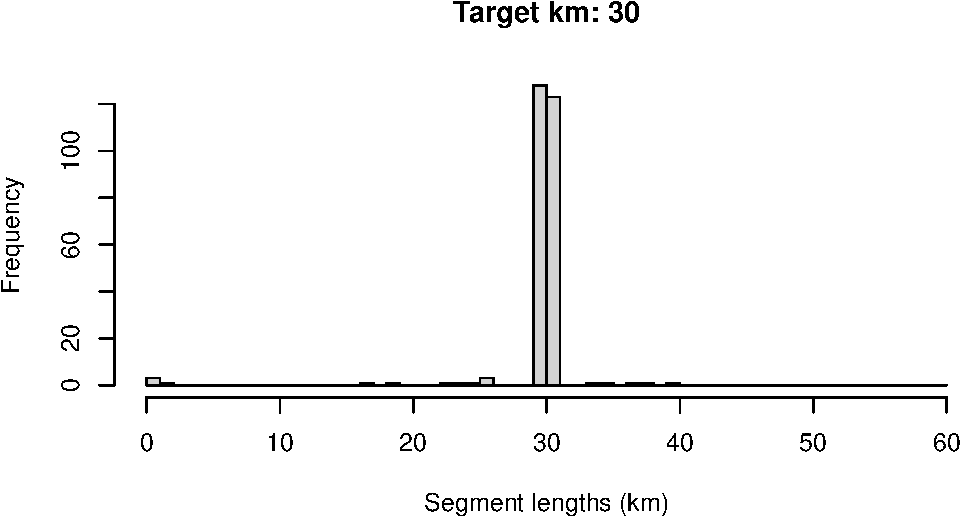
\includegraphics{figures/unnamed-chunk-38-1.pdf}

And the \texttt{das} slot holds the original \texttt{data.frame} of \texttt{DAS} data, modified slightly: the column \texttt{OnEffort} has been modified according to Beaufort range conditions, and the column \texttt{seg\_id} indicates which segment the event occurs within

\begin{Shaded}
\begin{Highlighting}[]
\NormalTok{cruz}\OperatorTok{$}\NormalTok{cohorts}\OperatorTok{$}\NormalTok{default}\OperatorTok{$}\NormalTok{density}\OperatorTok{$}\NormalTok{das }\OperatorTok\StringTok{ }\NormalTok{names}
\NormalTok{ [}\DecValTok{1}\NormalTok{] }\StringTok{"Event"}            \StringTok{"DateTime"}         \StringTok{"Lat"}              \StringTok{"Lon"}             
\NormalTok{ [}\DecValTok{5}\NormalTok{] }\StringTok{"OnEffort"}         \StringTok{"Cruise"}           \StringTok{"Mode"}             \StringTok{"OffsetGMT"}       
\NormalTok{ [}\DecValTok{9}\NormalTok{] }\StringTok{"EffType"}          \StringTok{"ESWsides"}         \StringTok{"Course"}           \StringTok{"SpdKt"}           
\NormalTok{[}\DecValTok{13}\NormalTok{] }\StringTok{"Bft"}              \StringTok{"SwellHght"}        \StringTok{"WindSpdKt"}        \StringTok{"RainFog"}         
\NormalTok{[}\DecValTok{17}\NormalTok{] }\StringTok{"HorizSun"}         \StringTok{"VertSun"}          \StringTok{"Glare"}            \StringTok{"Vis"}             
\NormalTok{[}\DecValTok{21}\NormalTok{] }\StringTok{"ObsL"}             \StringTok{"Rec"}              \StringTok{"ObsR"}             \StringTok{"ObsInd"}          
\NormalTok{[}\DecValTok{25}\NormalTok{] }\StringTok{"Data1"}            \StringTok{"Data2"}            \StringTok{"Data3"}            \StringTok{"Data4"}           
\NormalTok{[}\DecValTok{29}\NormalTok{] }\StringTok{"Data5"}            \StringTok{"Data6"}            \StringTok{"Data7"}            \StringTok{"Data8"}           
\NormalTok{[}\DecValTok{33}\NormalTok{] }\StringTok{"Data9"}            \StringTok{"Data10"}           \StringTok{"Data11"}           \StringTok{"Data12"}          
\NormalTok{[}\DecValTok{37}\NormalTok{] }\StringTok{"EffortDot"}        \StringTok{"EventNum"}         \StringTok{"file_das"}         \StringTok{"line_num"}        
\NormalTok{[}\DecValTok{41}\NormalTok{] }\StringTok{"stratum_HI_EEZ"}   \StringTok{"stratum_WHICEAS"}  \StringTok{"stratum_OtherCNP"} \StringTok{"study_area"}      
\NormalTok{[}\DecValTok{45}\NormalTok{] }\StringTok{"year"}             \StringTok{"month"}            \StringTok{"day"}              \StringTok{"yday"}            
\NormalTok{[}\DecValTok{49}\NormalTok{] }\StringTok{"km_int"}           \StringTok{"km_cum"}           \StringTok{"ship"}             \StringTok{"stratum"}         
\NormalTok{[}\DecValTok{53}\NormalTok{] }\StringTok{"seg_id"}           \StringTok{"use"}             
\end{Highlighting}
\end{Shaded}

The \texttt{segmentize()} function and its associated settings were designed to give researchers full control over how data are segmented, be it for design-based density analysis (which tend to use long segments of 100 km or more and allow for non-contiguous effort to be included in the same segment) or for habitat modeling (which tend to use short segments of 5 - 10 km and disallow non-contiguous effort to be pooled into the same segment). To demonstrate that versatility, checkout the \protect\hyperlink{segmentizing}{appendix on segmentizing}.

\hypertarget{process-sightings}{%
\subsection*{Process sightings}\label{process-sightings}}
\addcontentsline{toc}{subsection}{Process sightings}

To process sightings for each cohort of species, use the function \texttt{process\_sightings()}. This function has three basic steps: for each cohort, the function (1) prepares a sightings table using the function \texttt{das\_sight()} from \texttt{swfscDAS}; (2) filters those sightings to species codes specified for the cohort in your \texttt{settings} input; and (3) evaluates each of those sightings, asking if each should be included in the analysis according to your \texttt{settings}.

\begin{Shaded}
\begin{Highlighting}[]
\NormalTok{cruz <-}\StringTok{ }\KeywordTok{process_sightings}\NormalTok{(cruz)}
\end{Highlighting}
\end{Shaded}

The function produces a formatted dataset and adds it to a new \texttt{sightings} slot. It does this for each analysis (\texttt{density} and, if specified, \texttt{distance}) in each cohort.

\begin{Shaded}
\begin{Highlighting}[]
\NormalTok{cruz}\OperatorTok{$}\NormalTok{cohorts}\OperatorTok{$}\NormalTok{default}\OperatorTok{$}\NormalTok{density }\OperatorTok\StringTok{ }\NormalTok{names}
\NormalTok{[}\DecValTok{1}\NormalTok{] }\StringTok{"segments"}  \StringTok{"das"}       \StringTok{"sightings"}
\NormalTok{cruz}\OperatorTok{$}\NormalTok{cohorts}\OperatorTok{$}\NormalTok{fkw_insular}\OperatorTok{$}\NormalTok{density }\OperatorTok\StringTok{ }\NormalTok{names}
\NormalTok{[}\DecValTok{1}\NormalTok{] }\StringTok{"segments"}  \StringTok{"das"}       \StringTok{"sightings"}
\NormalTok{cruz}\OperatorTok{$}\NormalTok{cohorts}\OperatorTok{$}\NormalTok{fkw_insular}\OperatorTok{$}\NormalTok{distance }\OperatorTok\StringTok{ }\NormalTok{names}
\NormalTok{[}\DecValTok{1}\NormalTok{] }\StringTok{"segments"}  \StringTok{"das"}       \StringTok{"sightings"}
\end{Highlighting}
\end{Shaded}

Note that the \texttt{sightings} table has a column named \texttt{included} (\texttt{TRUE} = yes, use it in the analysis). Any sightings that do not meet the inclusion criteria as specified in your settings will be \texttt{included\ =\ FALSE}, but they won't be removed from the data.

Since the sightings in each cohort are processed slightly differently according to the cohort's specific settings, you should expect different numbers of included/excluded sightings in each cohort-analysis dataset:

\begin{Shaded}
\begin{Highlighting}[]
\NormalTok{cruz}\OperatorTok{$}\NormalTok{cohorts}\OperatorTok{$}\NormalTok{default}\OperatorTok{$}\NormalTok{density}\OperatorTok{$}\NormalTok{sightings}\OperatorTok{$}\NormalTok{included }\OperatorTok\StringTok{ }\NormalTok{table}
\NormalTok{.}
\OtherTok{FALSE}  \OtherTok{TRUE} 
  \DecValTok{123}   \DecValTok{205} 
\NormalTok{cruz}\OperatorTok{$}\NormalTok{cohorts}\OperatorTok{$}\NormalTok{fkw_insular}\OperatorTok{$}\NormalTok{density}\OperatorTok{$}\NormalTok{sightings}\OperatorTok{$}\NormalTok{included }\OperatorTok\StringTok{ }\NormalTok{table}
\NormalTok{.}
\OtherTok{FALSE}  \OtherTok{TRUE} 
    \DecValTok{1}     \DecValTok{3} 
\NormalTok{cruz}\OperatorTok{$}\NormalTok{cohorts}\OperatorTok{$}\NormalTok{fkw_insular}\OperatorTok{$}\NormalTok{distance}\OperatorTok{$}\NormalTok{sightings}\OperatorTok{$}\NormalTok{included }\OperatorTok\StringTok{ }\NormalTok{table}
\NormalTok{.}
\OtherTok{TRUE} 
   \DecValTok{4} 
\end{Highlighting}
\end{Shaded}

When this function's \texttt{verbose} argument is \texttt{TRUE} (the default), a message is printed each time a sighting does not meet the inclusion criteria (see above).

\hypertarget{sightings-data-structure}{%
\subsubsection*{Sightings data structure}\label{sightings-data-structure}}
\addcontentsline{toc}{subsubsection}{Sightings data structure}

The \texttt{sightings} table has many other variables:

\begin{Shaded}
\begin{Highlighting}[]
\NormalTok{cruz}\OperatorTok{$}\NormalTok{cohorts}\OperatorTok{$}\NormalTok{default}\OperatorTok{$}\NormalTok{density}\OperatorTok{$}\NormalTok{sightings }\OperatorTok\StringTok{ }\NormalTok{names}
\NormalTok{ [}\DecValTok{1}\NormalTok{] }\StringTok{"Event"}            \StringTok{"DateTime"}         \StringTok{"Lat"}              \StringTok{"Lon"}             
\NormalTok{ [}\DecValTok{5}\NormalTok{] }\StringTok{"OnEffort"}         \StringTok{"Cruise"}           \StringTok{"Mode"}             \StringTok{"OffsetGMT"}       
\NormalTok{ [}\DecValTok{9}\NormalTok{] }\StringTok{"EffType"}          \StringTok{"ESWsides"}         \StringTok{"Course"}           \StringTok{"SpdKt"}           
\NormalTok{[}\DecValTok{13}\NormalTok{] }\StringTok{"Bft"}              \StringTok{"SwellHght"}        \StringTok{"WindSpdKt"}        \StringTok{"RainFog"}         
\NormalTok{[}\DecValTok{17}\NormalTok{] }\StringTok{"HorizSun"}         \StringTok{"VertSun"}          \StringTok{"Glare"}            \StringTok{"Vis"}             
\NormalTok{[}\DecValTok{21}\NormalTok{] }\StringTok{"ObsL"}             \StringTok{"Rec"}              \StringTok{"ObsR"}             \StringTok{"ObsInd"}          
\NormalTok{[}\DecValTok{25}\NormalTok{] }\StringTok{"EffortDot"}        \StringTok{"EventNum"}         \StringTok{"file_das"}         \StringTok{"line_num"}        
\NormalTok{[}\DecValTok{29}\NormalTok{] }\StringTok{"stratum_HI_EEZ"}   \StringTok{"stratum_WHICEAS"}  \StringTok{"stratum_OtherCNP"} \StringTok{"study_area"}      
\NormalTok{[}\DecValTok{33}\NormalTok{] }\StringTok{"year"}             \StringTok{"month"}            \StringTok{"day"}              \StringTok{"yday"}            
\NormalTok{[}\DecValTok{37}\NormalTok{] }\StringTok{"km_int"}           \StringTok{"km_cum"}           \StringTok{"ship"}             \StringTok{"stratum"}         
\NormalTok{[}\DecValTok{41}\NormalTok{] }\StringTok{"seg_id"}           \StringTok{"use"}              \StringTok{"SightNo"}          \StringTok{"Subgroup"}        
\NormalTok{[}\DecValTok{45}\NormalTok{] }\StringTok{"SightNoDaily"}     \StringTok{"Obs"}              \StringTok{"ObsStd"}           \StringTok{"Bearing"}         
\NormalTok{[}\DecValTok{49}\NormalTok{] }\StringTok{"Reticle"}          \StringTok{"DistNm"}           \StringTok{"Cue"}              \StringTok{"Method"}          
\NormalTok{[}\DecValTok{53}\NormalTok{] }\StringTok{"Photos"}           \StringTok{"Birds"}            \StringTok{"CalibSchool"}      \StringTok{"PhotosAerial"}    
\NormalTok{[}\DecValTok{57}\NormalTok{] }\StringTok{"Biopsy"}           \StringTok{"CourseSchool"}     \StringTok{"TurtleSp"}         \StringTok{"TurtleGs"}        
\NormalTok{[}\DecValTok{61}\NormalTok{] }\StringTok{"TurtleJFR"}        \StringTok{"TurtleAge"}        \StringTok{"TurtleCapt"}       \StringTok{"PinnipedSp"}      
\NormalTok{[}\DecValTok{65}\NormalTok{] }\StringTok{"PinnipedGs"}       \StringTok{"BoatType"}         \StringTok{"BoatGs"}           \StringTok{"PerpDistKm"}      
\NormalTok{[}\DecValTok{69}\NormalTok{] }\StringTok{"species"}          \StringTok{"best"}             \StringTok{"low"}              \StringTok{"high"}            
\NormalTok{[}\DecValTok{73}\NormalTok{] }\StringTok{"prob"}             \StringTok{"mixed"}            \StringTok{"ss_tot"}           \StringTok{"ss_percent"}      
\NormalTok{[}\DecValTok{77}\NormalTok{] }\StringTok{"n_sp"}             \StringTok{"n_obs"}            \StringTok{"n_best"}           \StringTok{"n_low"}           
\NormalTok{[}\DecValTok{81}\NormalTok{] }\StringTok{"n_high"}           \StringTok{"calibr"}           \StringTok{"included"}        
\end{Highlighting}
\end{Shaded}

Columns 41 onwards correspond to sightings information. Columns of note:

\begin{itemize}
\item
  \texttt{species} (column 68) contains the species code. There is only one species-code per row (i.e, multi-species sightings have been expanded to multiple rows).
\item
  \texttt{best}, \texttt{low}, and \texttt{high} (columns 69- 71) contain the refined group size estimates, averaged across observers and calibrated according to the cohort's settings specifications. For multi-species sightings, these numbers represent the number of individuals for the single species represented in the row (i.e., the original group size estimate has been scaled by the percentage attritbuted to this species).
\item
  The columns following those group size estimates (\texttt{prob} through \texttt{calibr}) detail how group sizes were estimated: \texttt{prob} indicates whether probable species codes were accepted; \texttt{mixed} indicates whether this species' sighting is part of a mixed-species sighting; \texttt{n\_sp} provides the number of species occurring in this sighitng; \texttt{n\_obs} gives the number of observers who contributed group size estimates; \texttt{n\_best} through \texttt{n\_high} gives the number of valid group size estimates given; and \texttt{calibr} indicates whether or not calibration was attempted for this sighting based on the settings (see next section).
\item
  As explained above, the final column, \texttt{included}, indicates whether this species should be included in the analysis.
\end{itemize}

Here is a glimpse of the data:

\begin{Shaded}
\begin{Highlighting}[]
\NormalTok{cruz}\OperatorTok{$}\NormalTok{cohorts}\OperatorTok{$}\NormalTok{fkw_insular}\OperatorTok{$}\NormalTok{distance}\OperatorTok{$}\NormalTok{sightings }\OperatorTok\StringTok{ }\NormalTok{glimpse}
\NormalTok{Rows}\OperatorTok{:}\StringTok{ }\DecValTok{4}
\NormalTok{Columns}\OperatorTok{:}\StringTok{ }\DecValTok{83}
\OperatorTok{$}\StringTok{ }\NormalTok{Event            }\OperatorTok{<}\NormalTok{chr}\OperatorTok{>}\StringTok{ "S"}\NormalTok{, }\StringTok{"S"}\NormalTok{, }\StringTok{"S"}\NormalTok{, }\StringTok{"S"}
\OperatorTok{$}\StringTok{ }\NormalTok{DateTime         }\OperatorTok{<}\NormalTok{dttm}\OperatorTok{>}\StringTok{ }\DecValTok{2020-01-28} \DecValTok{16}\OperatorTok{:}\DecValTok{35}\OperatorTok{:}\DecValTok{09}\NormalTok{, }\DecValTok{2020-02-27} \DecValTok{11}\OperatorTok{:}\DecValTok{52}\OperatorTok{:}\DecValTok{38}\NormalTok{, }\DecValTok{2020-02-28} \OperatorTok{~}
\ErrorTok{$}\StringTok{ }\NormalTok{Lat              }\OperatorTok{<}\NormalTok{dbl}\OperatorTok{>}\StringTok{ }\FloatTok{20.80800}\NormalTok{, }\FloatTok{18.83133}\NormalTok{, }\FloatTok{19.13683}\NormalTok{, }\FloatTok{18.20767}
\OperatorTok{$}\StringTok{ }\NormalTok{Lon              }\OperatorTok{<}\NormalTok{dbl}\OperatorTok{>}\StringTok{ }\FloatTok{-158.3488}\NormalTok{, }\FloatTok{-157.1577}\NormalTok{, }\FloatTok{-156.3863}\NormalTok{, }\FloatTok{-154.7485}
\OperatorTok{$}\StringTok{ }\NormalTok{OnEffort         }\OperatorTok{<}\NormalTok{lgl}\OperatorTok{>}\StringTok{ }\OtherTok{TRUE}\NormalTok{, }\OtherTok{TRUE}\NormalTok{, }\OtherTok{TRUE}\NormalTok{, }\OtherTok{TRUE}
\OperatorTok{$}\StringTok{ }\NormalTok{Cruise           }\OperatorTok{<}\NormalTok{dbl}\OperatorTok{>}\StringTok{ }\DecValTok{2001}\NormalTok{, }\DecValTok{2001}\NormalTok{, }\DecValTok{2001}\NormalTok{, }\DecValTok{2001}
\OperatorTok{$}\StringTok{ }\NormalTok{Mode             }\OperatorTok{<}\NormalTok{chr}\OperatorTok{>}\StringTok{ "C"}\NormalTok{, }\StringTok{"C"}\NormalTok{, }\StringTok{"C"}\NormalTok{, }\StringTok{"C"}
\OperatorTok{$}\StringTok{ }\NormalTok{OffsetGMT        }\OperatorTok{<}\NormalTok{int}\OperatorTok{>}\StringTok{ }\DecValTok{-10}\NormalTok{, }\DecValTok{-10}\NormalTok{, }\DecValTok{-10}\NormalTok{, }\DecValTok{-10}
\OperatorTok{$}\StringTok{ }\NormalTok{EffType          }\OperatorTok{<}\NormalTok{chr}\OperatorTok{>}\StringTok{ "S"}\NormalTok{, }\StringTok{"S"}\NormalTok{, }\StringTok{"N"}\NormalTok{, }\StringTok{"S"}
\OperatorTok{$}\StringTok{ }\NormalTok{ESWsides         }\OperatorTok{<}\NormalTok{dbl}\OperatorTok{>}\StringTok{ }\DecValTok{2}\NormalTok{, }\DecValTok{2}\NormalTok{, }\DecValTok{2}\NormalTok{, }\DecValTok{2}
\OperatorTok{$}\StringTok{ }\NormalTok{Course           }\OperatorTok{<}\NormalTok{dbl}\OperatorTok{>}\StringTok{ }\DecValTok{122}\NormalTok{, }\DecValTok{285}\NormalTok{, }\DecValTok{90}\NormalTok{, }\DecValTok{107}
\OperatorTok{$}\StringTok{ }\NormalTok{SpdKt            }\OperatorTok{<}\NormalTok{dbl}\OperatorTok{>}\StringTok{ }\FloatTok{9.6}\NormalTok{, }\FloatTok{9.4}\NormalTok{, }\FloatTok{8.6}\NormalTok{, }\FloatTok{7.9}
\OperatorTok{$}\StringTok{ }\NormalTok{Bft              }\OperatorTok{<}\NormalTok{dbl}\OperatorTok{>}\StringTok{ }\DecValTok{3}\NormalTok{, }\DecValTok{5}\NormalTok{, }\DecValTok{5}\NormalTok{, }\DecValTok{6}
\OperatorTok{$}\StringTok{ }\NormalTok{SwellHght        }\OperatorTok{<}\NormalTok{dbl}\OperatorTok{>}\StringTok{ }\DecValTok{5}\NormalTok{, }\DecValTok{8}\NormalTok{, }\DecValTok{7}\NormalTok{, }\DecValTok{11}
\OperatorTok{$}\StringTok{ }\NormalTok{WindSpdKt        }\OperatorTok{<}\NormalTok{dbl}\OperatorTok{>}\StringTok{ }\DecValTok{10}\NormalTok{, }\DecValTok{17}\NormalTok{, }\DecValTok{17}\NormalTok{, }\DecValTok{24}
\OperatorTok{$}\StringTok{ }\NormalTok{RainFog          }\OperatorTok{<}\NormalTok{dbl}\OperatorTok{>}\StringTok{ }\DecValTok{5}\NormalTok{, }\DecValTok{5}\NormalTok{, }\DecValTok{5}\NormalTok{, }\DecValTok{5}
\OperatorTok{$}\StringTok{ }\NormalTok{HorizSun         }\OperatorTok{<}\NormalTok{dbl}\OperatorTok{>}\StringTok{ }\DecValTok{4}\NormalTok{, }\DecValTok{7}\NormalTok{, }\DecValTok{3}\NormalTok{, }\DecValTok{4}
\OperatorTok{$}\StringTok{ }\NormalTok{VertSun          }\OperatorTok{<}\NormalTok{dbl}\OperatorTok{>}\StringTok{ }\DecValTok{2}\NormalTok{, }\DecValTok{1}\NormalTok{, }\DecValTok{1}\NormalTok{, }\DecValTok{1}
\OperatorTok{$}\StringTok{ }\NormalTok{Glare            }\OperatorTok{<}\NormalTok{lgl}\OperatorTok{>}\StringTok{ }\OtherTok{FALSE}\NormalTok{, }\OtherTok{FALSE}\NormalTok{, }\OtherTok{FALSE}\NormalTok{, }\OtherTok{FALSE}
\OperatorTok{$}\StringTok{ }\NormalTok{Vis              }\OperatorTok{<}\NormalTok{dbl}\OperatorTok{>}\StringTok{ }\FloatTok{6.0}\NormalTok{, }\FloatTok{5.5}\NormalTok{, }\FloatTok{5.0}\NormalTok{, }\FloatTok{4.0}
\OperatorTok{$}\StringTok{ }\NormalTok{ObsL             }\OperatorTok{<}\NormalTok{chr}\OperatorTok{>}\StringTok{ "238"}\NormalTok{, }\StringTok{"238"}\NormalTok{, }\StringTok{"197"}\NormalTok{, }\StringTok{"125"}
\OperatorTok{$}\StringTok{ }\NormalTok{Rec              }\OperatorTok{<}\NormalTok{chr}\OperatorTok{>}\StringTok{ "125"}\NormalTok{, }\StringTok{"125"}\NormalTok{, }\StringTok{"227"}\NormalTok{, }\StringTok{"197"}
\OperatorTok{$}\StringTok{ }\NormalTok{ObsR             }\OperatorTok{<}\NormalTok{chr}\OperatorTok{>}\StringTok{ "197"}\NormalTok{, }\StringTok{"197"}\NormalTok{, }\StringTok{"126"}\NormalTok{, }\StringTok{"227"}
\OperatorTok{$}\StringTok{ }\NormalTok{ObsInd           }\OperatorTok{<}\NormalTok{chr}\OperatorTok{>}\StringTok{ }\OtherTok{NA}\NormalTok{, }\OtherTok{NA}\NormalTok{, }\OtherTok{NA}\NormalTok{, }\OtherTok{NA}
\OperatorTok{$}\StringTok{ }\NormalTok{EffortDot        }\OperatorTok{<}\NormalTok{lgl}\OperatorTok{>}\StringTok{ }\OtherTok{TRUE}\NormalTok{, }\OtherTok{TRUE}\NormalTok{, }\OtherTok{TRUE}\NormalTok{, }\OtherTok{TRUE}
\OperatorTok{$}\StringTok{ }\NormalTok{EventNum         }\OperatorTok{<}\NormalTok{chr}\OperatorTok{>}\StringTok{ "422"}\NormalTok{, }\StringTok{"213"}\NormalTok{, }\StringTok{"238"}\NormalTok{, }\StringTok{"371"}
\OperatorTok{$}\StringTok{ }\NormalTok{file_das         }\OperatorTok{<}\NormalTok{chr}\OperatorTok{>}\StringTok{ "HICEASwinter2020.das"}\NormalTok{, }\StringTok{"HICEASwinter2020.das"}\NormalTok{, }\StringTok{"HIC~}
\StringTok{$ line_num         <int> 5016, 15756, 16275, 18395}
\StringTok{$ stratum_HI_EEZ   <lgl> TRUE, TRUE, TRUE, TRUE}
\StringTok{$ stratum_WHICEAS  <lgl> TRUE, TRUE, TRUE, TRUE}
\StringTok{$ stratum_OtherCNP <lgl> TRUE, TRUE, TRUE, TRUE}
\StringTok{$ study_area       <lgl> TRUE, TRUE, TRUE, TRUE}
\StringTok{$ year             <dbl> 2020, 2020, 2020, 2020}
\StringTok{$ month            <dbl> 1, 2, 2, 3}
\StringTok{$ day              <int> 28, 27, 28, 3}
\StringTok{$ yday             <dbl> 28, 58, 59, 63}
\StringTok{$ km_int           <dbl> 0, 0, 0, 0}
\StringTok{$ km_cum           <dbl> 1646.400, 5375.415, 5560.489, 6239.292}
\StringTok{$ ship             <chr> "}\NormalTok{OES}\StringTok{", "}\NormalTok{OES}\StringTok{", "}\NormalTok{OES}\StringTok{", "}\NormalTok{OES}\StringTok{"}
\StringTok{$ stratum          <chr> "}\NormalTok{HI_EEZ}\OperatorTok{&}\NormalTok{WHICEAS}\OperatorTok{&}\NormalTok{OtherCNP}\StringTok{", "}\NormalTok{HI_EEZ}\OperatorTok{&}\NormalTok{WHICEAS}\OperatorTok{&}\NormalTok{OtherCNP}\StringTok{",~}
\StringTok{$ seg_id           <int> 158, 232, 111, 242}
\StringTok{$ use              <lgl> TRUE, TRUE, TRUE, TRUE}
\StringTok{$ SightNo          <chr> "}\DecValTok{131}\StringTok{", "}\DecValTok{255}\StringTok{", "}\DecValTok{258}\StringTok{", "}\DecValTok{285}\StringTok{"}
\StringTok{$ Subgroup         <chr> NA, NA, NA, NA}
\StringTok{$ SightNoDaily     <chr> "}\DecValTok{20200128}\NormalTok{_}\DecValTok{8}\StringTok{", "}\DecValTok{20200227}\NormalTok{_}\DecValTok{19}\StringTok{", "}\DecValTok{20200228}\NormalTok{_}\DecValTok{18}\StringTok{", "}\DecValTok{20200303}\OperatorTok{~}
\ErrorTok{$}\StringTok{ }\NormalTok{Obs              }\OperatorTok{<}\NormalTok{chr}\OperatorTok{>}\StringTok{ "197"}\NormalTok{, }\StringTok{"125"}\NormalTok{, }\StringTok{"126"}\NormalTok{, }\StringTok{"125"}
\OperatorTok{$}\StringTok{ }\NormalTok{ObsStd           }\OperatorTok{<}\NormalTok{lgl}\OperatorTok{>}\StringTok{ }\OtherTok{TRUE}\NormalTok{, }\OtherTok{TRUE}\NormalTok{, }\OtherTok{TRUE}\NormalTok{, }\OtherTok{TRUE}
\OperatorTok{$}\StringTok{ }\NormalTok{Bearing          }\OperatorTok{<}\NormalTok{dbl}\OperatorTok{>}\StringTok{ }\DecValTok{79}\NormalTok{, }\DecValTok{0}\NormalTok{, }\DecValTok{15}\NormalTok{, }\DecValTok{314}
\OperatorTok{$}\StringTok{ }\NormalTok{Reticle          }\OperatorTok{<}\NormalTok{dbl}\OperatorTok{>}\StringTok{ }\FloatTok{1.8}\NormalTok{, }\OtherTok{NA}\NormalTok{, }\FloatTok{1.5}\NormalTok{, }\FloatTok{5.0}
\OperatorTok{$}\StringTok{ }\NormalTok{DistNm           }\OperatorTok{<}\NormalTok{dbl}\OperatorTok{>}\StringTok{ }\FloatTok{1.88}\NormalTok{, }\FloatTok{0.20}\NormalTok{, }\FloatTok{2.09}\NormalTok{, }\FloatTok{0.92}
\OperatorTok{$}\StringTok{ }\NormalTok{Cue              }\OperatorTok{<}\NormalTok{dbl}\OperatorTok{>}\StringTok{ }\DecValTok{3}\NormalTok{, }\DecValTok{2}\NormalTok{, }\DecValTok{3}\NormalTok{, }\DecValTok{3}
\OperatorTok{$}\StringTok{ }\NormalTok{Method           }\OperatorTok{<}\NormalTok{dbl}\OperatorTok{>}\StringTok{ }\DecValTok{4}\NormalTok{, }\DecValTok{1}\NormalTok{, }\DecValTok{4}\NormalTok{, }\DecValTok{4}
\OperatorTok{$}\StringTok{ }\NormalTok{Photos           }\OperatorTok{<}\NormalTok{chr}\OperatorTok{>}\StringTok{ "Y"}\NormalTok{, }\StringTok{"N"}\NormalTok{, }\StringTok{"Y"}\NormalTok{, }\StringTok{"N"}
\OperatorTok{$}\StringTok{ }\NormalTok{Birds            }\OperatorTok{<}\NormalTok{chr}\OperatorTok{>}\StringTok{ "N"}\NormalTok{, }\StringTok{"N"}\NormalTok{, }\StringTok{"N"}\NormalTok{, }\StringTok{"N"}
\OperatorTok{$}\StringTok{ }\NormalTok{CalibSchool      }\OperatorTok{<}\NormalTok{chr}\OperatorTok{>}\StringTok{ "N"}\NormalTok{, }\StringTok{"N"}\NormalTok{, }\StringTok{"N"}\NormalTok{, }\StringTok{"N"}
\OperatorTok{$}\StringTok{ }\NormalTok{PhotosAerial     }\OperatorTok{<}\NormalTok{chr}\OperatorTok{>}\StringTok{ "N"}\NormalTok{, }\StringTok{"N"}\NormalTok{, }\StringTok{"N"}\NormalTok{, }\StringTok{"N"}
\OperatorTok{$}\StringTok{ }\NormalTok{Biopsy           }\OperatorTok{<}\NormalTok{chr}\OperatorTok{>}\StringTok{ "N"}\NormalTok{, }\StringTok{"N"}\NormalTok{, }\StringTok{"N"}\NormalTok{, }\StringTok{"N"}
\OperatorTok{$}\StringTok{ }\NormalTok{CourseSchool     }\OperatorTok{<}\NormalTok{dbl}\OperatorTok{>}\StringTok{ }\OtherTok{NA}\NormalTok{, }\OtherTok{NA}\NormalTok{, }\OtherTok{NA}\NormalTok{, }\OtherTok{NA}
\OperatorTok{$}\StringTok{ }\NormalTok{TurtleSp         }\OperatorTok{<}\NormalTok{chr}\OperatorTok{>}\StringTok{ }\OtherTok{NA}\NormalTok{, }\OtherTok{NA}\NormalTok{, }\OtherTok{NA}\NormalTok{, }\OtherTok{NA}
\OperatorTok{$}\StringTok{ }\NormalTok{TurtleGs         }\OperatorTok{<}\NormalTok{dbl}\OperatorTok{>}\StringTok{ }\OtherTok{NA}\NormalTok{, }\OtherTok{NA}\NormalTok{, }\OtherTok{NA}\NormalTok{, }\OtherTok{NA}
\OperatorTok{$}\StringTok{ }\NormalTok{TurtleJFR        }\OperatorTok{<}\NormalTok{chr}\OperatorTok{>}\StringTok{ }\OtherTok{NA}\NormalTok{, }\OtherTok{NA}\NormalTok{, }\OtherTok{NA}\NormalTok{, }\OtherTok{NA}
\OperatorTok{$}\StringTok{ }\NormalTok{TurtleAge        }\OperatorTok{<}\NormalTok{chr}\OperatorTok{>}\StringTok{ }\OtherTok{NA}\NormalTok{, }\OtherTok{NA}\NormalTok{, }\OtherTok{NA}\NormalTok{, }\OtherTok{NA}
\OperatorTok{$}\StringTok{ }\NormalTok{TurtleCapt       }\OperatorTok{<}\NormalTok{chr}\OperatorTok{>}\StringTok{ }\OtherTok{NA}\NormalTok{, }\OtherTok{NA}\NormalTok{, }\OtherTok{NA}\NormalTok{, }\OtherTok{NA}
\OperatorTok{$}\StringTok{ }\NormalTok{PinnipedSp       }\OperatorTok{<}\NormalTok{chr}\OperatorTok{>}\StringTok{ }\OtherTok{NA}\NormalTok{, }\OtherTok{NA}\NormalTok{, }\OtherTok{NA}\NormalTok{, }\OtherTok{NA}
\OperatorTok{$}\StringTok{ }\NormalTok{PinnipedGs       }\OperatorTok{<}\NormalTok{dbl}\OperatorTok{>}\StringTok{ }\OtherTok{NA}\NormalTok{, }\OtherTok{NA}\NormalTok{, }\OtherTok{NA}\NormalTok{, }\OtherTok{NA}
\OperatorTok{$}\StringTok{ }\NormalTok{BoatType         }\OperatorTok{<}\NormalTok{chr}\OperatorTok{>}\StringTok{ }\OtherTok{NA}\NormalTok{, }\OtherTok{NA}\NormalTok{, }\OtherTok{NA}\NormalTok{, }\OtherTok{NA}
\OperatorTok{$}\StringTok{ }\NormalTok{BoatGs           }\OperatorTok{<}\NormalTok{dbl}\OperatorTok{>}\StringTok{ }\OtherTok{NA}\NormalTok{, }\OtherTok{NA}\NormalTok{, }\OtherTok{NA}\NormalTok{, }\OtherTok{NA}
\OperatorTok{$}\StringTok{ }\NormalTok{PerpDistKm       }\OperatorTok{<}\NormalTok{dbl}\OperatorTok{>}\StringTok{ }\FloatTok{3.417790}\NormalTok{, }\FloatTok{0.000000}\NormalTok{, }\FloatTok{1.001806}\NormalTok{, }\FloatTok{1.225640}
\OperatorTok{$}\StringTok{ }\NormalTok{species          }\OperatorTok{<}\NormalTok{chr}\OperatorTok{>}\StringTok{ "033"}\NormalTok{, }\StringTok{"033"}\NormalTok{, }\StringTok{"033"}\NormalTok{, }\StringTok{"033"}
\OperatorTok{$}\StringTok{ }\NormalTok{best             }\OperatorTok{<}\NormalTok{dbl}\OperatorTok{>}\StringTok{ }\FloatTok{35.096667}\NormalTok{, }\FloatTok{1.000000}\NormalTok{, }\FloatTok{13.913043}\NormalTok{, }\FloatTok{6.956522}
\OperatorTok{$}\StringTok{ }\NormalTok{low              }\OperatorTok{<}\NormalTok{dbl}\OperatorTok{>}\StringTok{ }\FloatTok{19.672365}\NormalTok{, }\OtherTok{NA}\NormalTok{, }\FloatTok{9.165151}\NormalTok{, }\FloatTok{5.000000}
\OperatorTok{$}\StringTok{ }\NormalTok{high             }\OperatorTok{<}\NormalTok{dbl}\OperatorTok{>}\StringTok{ }\FloatTok{43.42268}\NormalTok{, }\OtherTok{NA}\NormalTok{, }\FloatTok{16.58312}\NormalTok{, }\FloatTok{20.00000}
\OperatorTok{$}\StringTok{ }\NormalTok{prob             }\OperatorTok{<}\NormalTok{lgl}\OperatorTok{>}\StringTok{ }\OtherTok{FALSE}\NormalTok{, }\OtherTok{FALSE}\NormalTok{, }\OtherTok{FALSE}\NormalTok{, }\OtherTok{FALSE}
\OperatorTok{$}\StringTok{ }\NormalTok{mixed            }\OperatorTok{<}\NormalTok{lgl}\OperatorTok{>}\StringTok{ }\OtherTok{FALSE}\NormalTok{, }\OtherTok{FALSE}\NormalTok{, }\OtherTok{FALSE}\NormalTok{, }\OtherTok{FALSE}
\OperatorTok{$}\StringTok{ }\NormalTok{ss_tot           }\OperatorTok{<}\NormalTok{dbl}\OperatorTok{>}\StringTok{ }\FloatTok{35.096667}\NormalTok{, }\FloatTok{1.000000}\NormalTok{, }\FloatTok{13.913043}\NormalTok{, }\FloatTok{6.956522}
\OperatorTok{$}\StringTok{ }\NormalTok{ss_percent       }\OperatorTok{<}\NormalTok{dbl}\OperatorTok{>}\StringTok{ }\DecValTok{1}\NormalTok{, }\OtherTok{NaN}\NormalTok{, }\DecValTok{1}\NormalTok{, }\DecValTok{1}
\OperatorTok{$}\StringTok{ }\NormalTok{n_sp             }\OperatorTok{<}\NormalTok{dbl}\OperatorTok{>}\StringTok{ }\DecValTok{1}\NormalTok{, }\DecValTok{1}\NormalTok{, }\DecValTok{1}\NormalTok{, }\DecValTok{1}
\OperatorTok{$}\StringTok{ }\NormalTok{n_obs            }\OperatorTok{<}\NormalTok{int}\OperatorTok{>}\StringTok{ }\DecValTok{3}\NormalTok{, }\DecValTok{1}\NormalTok{, }\DecValTok{2}\NormalTok{, }\DecValTok{1}
\OperatorTok{$}\StringTok{ }\NormalTok{n_best           }\OperatorTok{<}\NormalTok{int}\OperatorTok{>}\StringTok{ }\DecValTok{3}\NormalTok{, }\DecValTok{0}\NormalTok{, }\DecValTok{2}\NormalTok{, }\DecValTok{1}
\OperatorTok{$}\StringTok{ }\NormalTok{n_low            }\OperatorTok{<}\NormalTok{int}\OperatorTok{>}\StringTok{ }\DecValTok{3}\NormalTok{, }\DecValTok{0}\NormalTok{, }\DecValTok{2}\NormalTok{, }\DecValTok{1}
\OperatorTok{$}\StringTok{ }\NormalTok{n_high           }\OperatorTok{<}\NormalTok{int}\OperatorTok{>}\StringTok{ }\DecValTok{3}\NormalTok{, }\DecValTok{0}\NormalTok{, }\DecValTok{2}\NormalTok{, }\DecValTok{1}
\OperatorTok{$}\StringTok{ }\NormalTok{calibr           }\OperatorTok{<}\NormalTok{lgl}\OperatorTok{>}\StringTok{ }\OtherTok{TRUE}\NormalTok{, }\OtherTok{TRUE}\NormalTok{, }\OtherTok{TRUE}\NormalTok{, }\OtherTok{TRUE}
\OperatorTok{$}\StringTok{ }\NormalTok{included         }\OperatorTok{<}\NormalTok{lgl}\OperatorTok{>}\StringTok{ }\OtherTok{TRUE}\NormalTok{, }\OtherTok{TRUE}\NormalTok{, }\OtherTok{TRUE}\NormalTok{, }\OtherTok{TRUE}
\end{Highlighting}
\end{Shaded}

Note that the \texttt{process\_sightings()} function draws upon \texttt{cruz\$settings} for inclusion criteria, but some of those settings can be overridden with the function's manual inputs if you want to explore your options (see below).

\hypertarget{ss_calibration}{%
\subsubsection*{School size estimates}\label{ss_calibration}}
\addcontentsline{toc}{subsubsection}{School size estimates}

In the settings we are using in this tutorial, school size estimates are adjusted using the calibration models from \href{https://scholar.google.com/scholar?hl=en\&as_sdt=0\%2C43\&q=barlow+1998+group+size+caliration\&btnG=}{Barlow, Gerrodette, and Perryman (1998)} (their analysis is refined slightly and further explained in \href{https://scholar.google.com/scholar?hl=en\&as_sdt=0\%2C43\&q=barlow+1998+group+size+caliration\&btnG=}{Gerrodette, Perryman and Barlow, 2002}). These calibration corrections are observer-specific. Some observers tend to underestimate school size and their estimates are adjusted up; others tend to overestimate and their estimates are adjusted down. Some observers do not have calibration coefficients, and for them a generic adjustment (upwards, by dividing estimates by 0.8625) is used. Each observer's estimate is calibrated, then all observer estimates are averaged. To do that averaging, our \texttt{settings} specify that we shall use a geometric weighted mean, instead of an arithmetic mean, that weights school size estimates from multiple observers according to the variance of their calibration coefficients.

Here are our current best estimates of school size:

\begin{Shaded}
\begin{Highlighting}[]
\NormalTok{cruz}\OperatorTok{$}\NormalTok{cohorts}\OperatorTok{$}\NormalTok{default}\OperatorTok{$}\NormalTok{density}\OperatorTok{$}\NormalTok{sightings}\OperatorTok{$}\NormalTok{best }\OperatorTok\StringTok{ }\KeywordTok{head}\NormalTok{(}\DecValTok{20}\NormalTok{)}
\NormalTok{ [}\DecValTok{1}\NormalTok{]  }\FloatTok{1.1594203} \FloatTok{19.1620266}  \FloatTok{3.4702883}  \FloatTok{1.1594203}  \FloatTok{2.3188406}  \FloatTok{2.3188406}
\NormalTok{ [}\DecValTok{7}\NormalTok{]  }\FloatTok{2.3188406}  \FloatTok{3.4782609}  \FloatTok{2.3188406}  \FloatTok{2.3188406}  \FloatTok{1.1594203}  \FloatTok{1.1594203}
\NormalTok{[}\DecValTok{13}\NormalTok{]  }\FloatTok{0.9370535} \FloatTok{73.2878434}  \FloatTok{1.1594203}  \FloatTok{1.1594203}  \FloatTok{4.6376812}  \FloatTok{7.7776277}
\NormalTok{[}\DecValTok{19}\NormalTok{]  }\FloatTok{1.1594203}  \FloatTok{1.1594203}
\end{Highlighting}
\end{Shaded}

Let's compare those estimates to unadjusted ones, in which calibration (and therefore weighted geometric mean) is turned off:

\begin{Shaded}
\begin{Highlighting}[]
\NormalTok{cruz_demo <-}\StringTok{ }\KeywordTok{process_sightings}\NormalTok{(cruz, }
                               \DataTypeTok{calibrate =} \OtherTok{FALSE}\NormalTok{,}
                               \DataTypeTok{verbose =} \OtherTok{FALSE}\NormalTok{)}
\NormalTok{cruz_demo}\OperatorTok{$}\NormalTok{cohorts}\OperatorTok{$}\NormalTok{default}\OperatorTok{$}\NormalTok{density}\OperatorTok{$}\NormalTok{sightings}\OperatorTok{$}\NormalTok{best }\OperatorTok\StringTok{ }\KeywordTok{head}\NormalTok{(}\DecValTok{20}\NormalTok{)}
\NormalTok{ [}\DecValTok{1}\NormalTok{]  }\FloatTok{1.000000} \FloatTok{19.077486}  \FloatTok{3.454978}  \FloatTok{1.000000}  \FloatTok{2.000000}  \FloatTok{2.000000}  \FloatTok{2.000000}
\NormalTok{ [}\DecValTok{8}\NormalTok{]  }\FloatTok{3.000000}  \FloatTok{2.000000}  \FloatTok{2.000000}  \FloatTok{1.000000}  \FloatTok{1.000000}  \FloatTok{1.000000} \FloatTok{62.970508}
\NormalTok{[}\DecValTok{15}\NormalTok{]  }\FloatTok{1.000000}  \FloatTok{1.000000}  \FloatTok{4.000000}  \FloatTok{6.708204}  \FloatTok{1.000000}  \FloatTok{1.000000}
\end{Highlighting}
\end{Shaded}

Note that, since calibration is only used for schools above a certain size, the difference between calibration and non-calibrated estimates becomes clearer in larger groups.

You can also carry out calibration corrections without using a geometric weighted mean (the arithmetic mean will be used instead):

\begin{Shaded}
\begin{Highlighting}[]
\NormalTok{cruz_demo <-}\StringTok{ }\KeywordTok{process_sightings}\NormalTok{(cruz, }
                               \DataTypeTok{calibrate =} \OtherTok{TRUE}\NormalTok{,}
                               \DataTypeTok{geometric_mean =} \OtherTok{FALSE}\NormalTok{,}
                               \DataTypeTok{verbose =} \OtherTok{FALSE}\NormalTok{)}

\NormalTok{cruz_demo}\OperatorTok{$}\NormalTok{cohorts}\OperatorTok{$}\NormalTok{default}\OperatorTok{$}\NormalTok{density}\OperatorTok{$}\NormalTok{sightings}\OperatorTok{$}\NormalTok{best }\OperatorTok\StringTok{ }\KeywordTok{head}\NormalTok{(}\DecValTok{20}\NormalTok{)}
\NormalTok{ [}\DecValTok{1}\NormalTok{]  }\FloatTok{1.1594203} \FloatTok{22.7906203}  \FloatTok{4.1274352}  \FloatTok{1.1594203}  \FloatTok{2.3188406}  \FloatTok{2.3188406}
\NormalTok{ [}\DecValTok{7}\NormalTok{]  }\FloatTok{2.3188406}  \FloatTok{3.4782609}  \FloatTok{2.3188406}  \FloatTok{2.3188406}  \FloatTok{1.1594203}  \FloatTok{1.1594203}
\NormalTok{[}\DecValTok{13}\NormalTok{]  }\FloatTok{0.9370535} \FloatTok{89.9371981}  \FloatTok{1.1594203}  \FloatTok{1.1594203}  \FloatTok{4.6376812}  \FloatTok{8.1159420}
\NormalTok{[}\DecValTok{19}\NormalTok{]  }\FloatTok{1.1594203}  \FloatTok{1.1594203}
\end{Highlighting}
\end{Shaded}

Note that when \texttt{geometric\_mean\ =\ TRUE} but calibration is not carried out, the simple geometric mean is calculated instead of the \emph{weighted} geometric mean, since the weights are the variance estimates from the calibration routine.

Also note that school size calibration is only carried out if \texttt{settings\$group\_size\_calibration} is not \texttt{NULL}. However, even when calibration coefficients \emph{are} provided, it is possible to specify that calibration should only be carried out for raw estimates above a minimum threshold (see cohort setting \texttt{calibration\_floor}, whose default is \texttt{0}), since observers may be unlikely to mis-estimate the school size of a lone whale or pair. For observers who have calibration coefficients in the \texttt{settings\$group\_size\_coefficients} table, that minimum is specified for each observer individually. For observers not in that table, calibration will only be applied to raw school size estimates above \texttt{settings\$cohorts{[}{[}i{]}{]}\$calibration\_floor} or above.

\hypertarget{subgroups}{%
\subsubsection*{Subgroup size estimates}\label{subgroups}}
\addcontentsline{toc}{subsubsection}{Subgroup size estimates}

After sightings data are processed, the \texttt{process\_surveys()} function calls the subroutine \texttt{process\_subgroups()} to find and calculate subgroup school size estimates for false killer whales, if any occur in the \texttt{DAS} data (Event code ``\texttt{G}''). If subgroups are found, a \texttt{subgroups} slot is added to the analysis list for a cohort. This \texttt{subgroups} slot holds a list with three dataframes: \texttt{events} (each row is a school size estimate for a single subgroup during a single phase -- 1 or 2 -- within a single sighting); \texttt{subgroups} (each row is a single phase for a single subgroup, with all school size estimates averaged together (both arithmetically and geometrically); and \texttt{sightings} (each row is a school size estimate for a single phase for a single sighting, with all subgroup school sizes summed together). Examples of these datasets will be provided at a later date.

\hypertarget{review}{%
\section*{Review}\label{review}}
\addcontentsline{toc}{section}{Review}

By the end of this process, you have a single data object, \texttt{cruz}, with all the data you need to move forward into the next stages of mapping and analysis.

\begin{Shaded}
\begin{Highlighting}[]
\NormalTok{cruz }\OperatorTok\StringTok{ }\NormalTok{names }
\NormalTok{[}\DecValTok{1}\NormalTok{] }\StringTok{"settings"}   \StringTok{"strata"}     \StringTok{"study_area"} \StringTok{"cohorts"}   
\end{Highlighting}
\end{Shaded}

Each species-specific cohort has its own list under \texttt{cruz\$cohorts}:

\begin{Shaded}
\begin{Highlighting}[]
\NormalTok{cruz}\OperatorTok{$}\NormalTok{cohorts }\OperatorTok\StringTok{ }\NormalTok{names }
\NormalTok{[}\DecValTok{1}\NormalTok{] }\StringTok{"default"}     \StringTok{"fkw_insular"}
\end{Highlighting}
\end{Shaded}

Each of these cohorts can have two lists, \texttt{density} and \texttt{distance}, which contain the data to be used in those density estimation and detection function estimation, respectively:

\begin{Shaded}
\begin{Highlighting}[]
\KeywordTok{str}\NormalTok{(cruz}\OperatorTok{$}\NormalTok{cohorts,}
    \DataTypeTok{max.level=}\DecValTok{2}\NormalTok{,}
    \DataTypeTok{list.len =} \DecValTok{10}\NormalTok{,}
    \DataTypeTok{vec.len =} \DecValTok{0}\NormalTok{,}
    \DataTypeTok{give.length =} \OtherTok{FALSE}\NormalTok{,}
    \DataTypeTok{give.attr =} \OtherTok{FALSE}\NormalTok{)}
\NormalTok{List of }\DecValTok{2}
 \OperatorTok{$}\StringTok{ }\NormalTok{default    }\OperatorTok{:}\NormalTok{List of }\DecValTok{1}
\NormalTok{  ..}\OperatorTok{$}\StringTok{ }\NormalTok{density}\OperatorTok{:}\NormalTok{List of }\DecValTok{3}
 \OperatorTok{$}\StringTok{ }\NormalTok{fkw_insular}\OperatorTok{:}\NormalTok{List of }\DecValTok{2}
\NormalTok{  ..}\OperatorTok{$}\StringTok{ }\NormalTok{density }\OperatorTok{:}\NormalTok{List of }\DecValTok{3}
\NormalTok{  ..}\OperatorTok{$}\StringTok{ }\NormalTok{distance}\OperatorTok{:}\NormalTok{List of }\DecValTok{3}
\end{Highlighting}
\end{Shaded}

Each of these \texttt{analysis} slots is a list with the same elements:

\begin{Shaded}
\begin{Highlighting}[]
\NormalTok{cruz}\OperatorTok{$}\NormalTok{cohorts}\OperatorTok{$}\NormalTok{default}\OperatorTok{$}\NormalTok{density }\OperatorTok\StringTok{ }\NormalTok{names}
\NormalTok{[}\DecValTok{1}\NormalTok{] }\StringTok{"segments"}  \StringTok{"das"}       \StringTok{"sightings"}
\end{Highlighting}
\end{Shaded}

\begin{itemize}
\item
  \texttt{segments} is a summary table of segments.
\item
  \texttt{das} is the raw \texttt{DAS} data, modified with \texttt{seg\_id} to associate each row with a segment.
\item
  \texttt{sightings} is a dataframe of sightings processed according to this cohort's settings.
\end{itemize}

In each dataframes for each cohort-analysis (e.g., \texttt{default\$density}), there are three critically important columns to keep in mind:

\begin{itemize}
\item
  \textbf{\texttt{seg\_id}}: this column is used to indicate the segment ID a row of data belongs to.
\item
  \textbf{\texttt{use}}: this column indicates whether a row of effort should be used in the analysis. Every row of data within a single segment with have the same \texttt{use} value.
\item
  \textbf{\texttt{included}}: this column occurs in the \texttt{sightings} dataframe only. It indicates whether the sightings should be included in the analysis based on the specified settings. Any sighting with \texttt{use\ ==\ FALSE} will also have \texttt{included\ ==\ FALSE}, but it \emph{is} possible for sightings to have \texttt{use\ ==\ TRUE} with \texttt{included\ ==\ FALSE}. For example, if the setting \texttt{abeam\_sightings} is set to \texttt{FALSE}, a sighting with a bearing angle beyond the ship's beam can be excluded from the analysis (\texttt{included\ ==\ FALSE}) even though the effort segment it occurs within will still be used (\texttt{use\ ==\ TRUE}).
\end{itemize}

\hypertarget{maps}{%
\chapter{Maps}\label{maps}}

To build a flexible system for mapping cruise data, we have the following functions:

\hypertarget{publishable-maps}{%
\section*{Publishable maps}\label{publishable-maps}}
\addcontentsline{toc}{section}{Publishable maps}

\hypertarget{base-maps}{%
\subsection*{Base maps}\label{base-maps}}
\addcontentsline{toc}{subsection}{Base maps}

Begin with a basic map, including EEZ borders:

\begin{Shaded}
\begin{Highlighting}[]
\NormalTok{m <-}\StringTok{ }\KeywordTok{map_base}\NormalTok{(}\DataTypeTok{region=}\StringTok{'cnp'}\NormalTok{)}
\NormalTok{m}
\end{Highlighting}
\end{Shaded}

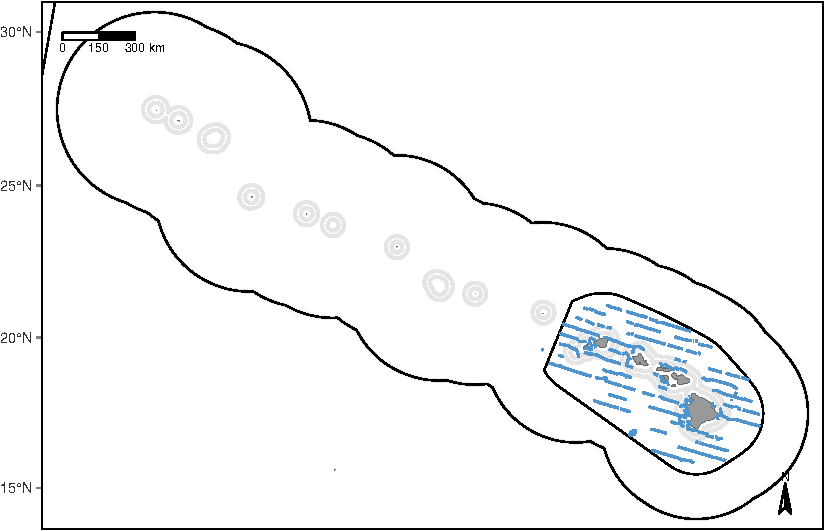
\includegraphics{figures/unnamed-chunk-54-1.pdf}

We also have a base map for the California Current \ldots{}

\begin{Shaded}
\begin{Highlighting}[]
\NormalTok{m <-}\StringTok{ }\KeywordTok{map_base}\NormalTok{(}\DataTypeTok{region=}\StringTok{'ccs'}\NormalTok{)}
\NormalTok{m}
\end{Highlighting}
\end{Shaded}

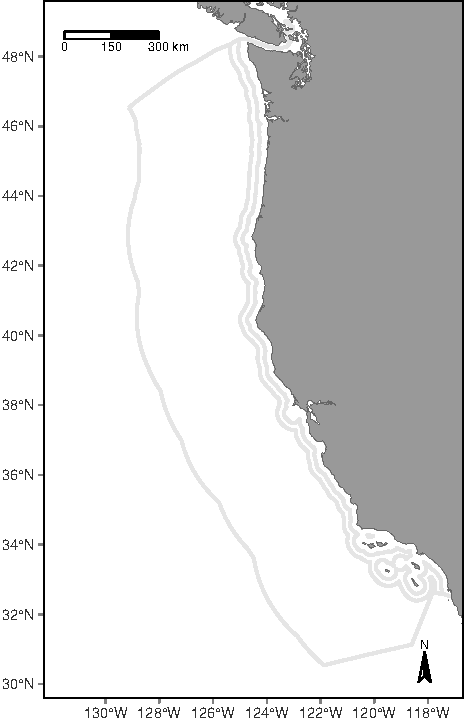
\includegraphics{figures/unnamed-chunk-55-1.pdf}

And the ETP:

\begin{Shaded}
\begin{Highlighting}[]
\NormalTok{m <-}\StringTok{ }\KeywordTok{map_base}\NormalTok{(}\DataTypeTok{region=}\StringTok{'etp'}\NormalTok{)}
\NormalTok{m}
\end{Highlighting}
\end{Shaded}

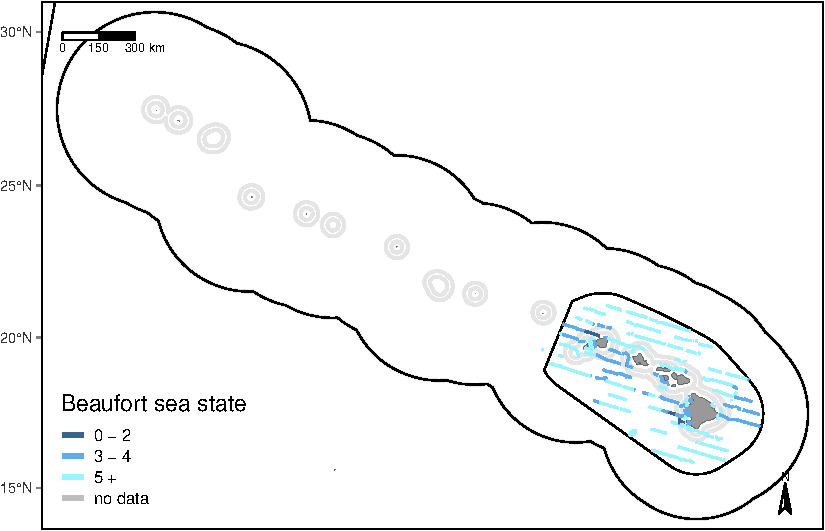
\includegraphics{figures/unnamed-chunk-56-1.pdf}

\hypertarget{add-strata}{%
\subsection*{Add strata}\label{add-strata}}
\addcontentsline{toc}{subsection}{Add strata}

Add your research strata to your map:

\begin{Shaded}
\begin{Highlighting}[]
\NormalTok{m <-}\StringTok{ }\KeywordTok{map_base}\NormalTok{(}\DataTypeTok{region=}\StringTok{'cnp'}\NormalTok{)}
\NormalTok{m <-}\StringTok{ }\KeywordTok{map_strata}\NormalTok{(m, }
\NormalTok{                cruz}\OperatorTok{$}\NormalTok{settings, }
                \DataTypeTok{region=}\StringTok{'cnp'}\NormalTok{)}
\NormalTok{m}
\end{Highlighting}
\end{Shaded}

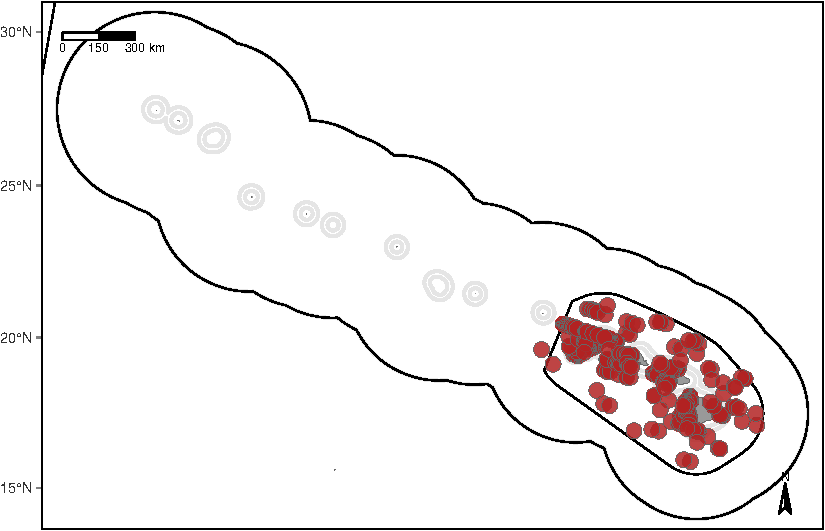
\includegraphics{figures/unnamed-chunk-57-1.pdf}

\hypertarget{add-survey-tracks}{%
\subsection*{Add survey tracks}\label{add-survey-tracks}}
\addcontentsline{toc}{subsection}{Add survey tracks}

\begin{Shaded}
\begin{Highlighting}[]
\NormalTok{m1 <-}\StringTok{ }\KeywordTok{map_effort}\NormalTok{(m, cruz)}
\NormalTok{m1}
\end{Highlighting}
\end{Shaded}

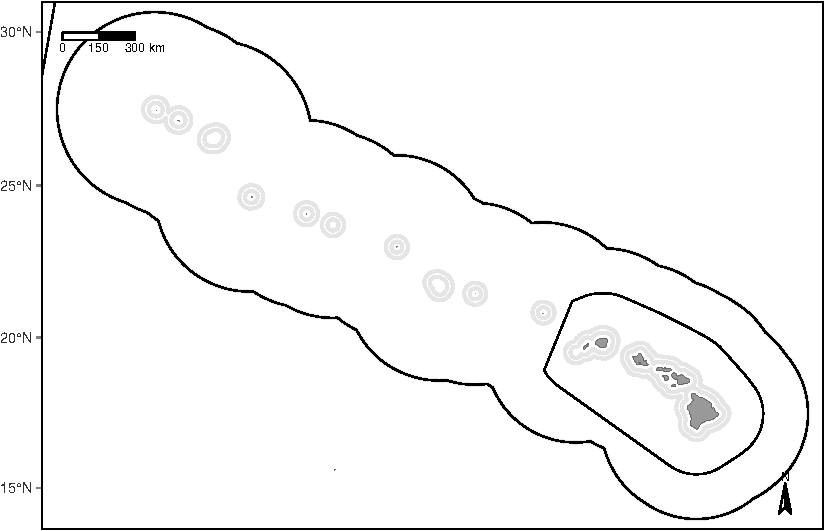
\includegraphics{figures/unnamed-chunk-58-1.pdf}

The defaults of \texttt{map\_effort()} assume, for simplicity, that you want to see the segments to be included in density estimation for the first cohort specified in your settings. You can adjust this and other defaults using the function arguments.

\hypertarget{customizing-effort}{%
\subsubsection*{Customizing effort}\label{customizing-effort}}
\addcontentsline{toc}{subsubsection}{Customizing effort}

\hypertarget{inputs}{%
\paragraph{Inputs}\label{inputs}}
\addcontentsline{toc}{paragraph}{Inputs}

To demonstrate some of the customization options, consider this map that shows segments to be \emph{excluded} from the \texttt{"distance"} (detection function) analysis for our second cohort (\texttt{fkw\_insular}).

\begin{Shaded}
\begin{Highlighting}[]
\KeywordTok{map_effort}\NormalTok{(m, cruz,}
           \DataTypeTok{cohort =} \DecValTok{2}\NormalTok{,}
           \DataTypeTok{analysis =} \StringTok{'distance'}\NormalTok{,}
           \DataTypeTok{use_type =} \KeywordTok{c}\NormalTok{(}\OtherTok{FALSE}\NormalTok{),}
           \DataTypeTok{effort_color=}\StringTok{'firebrick'}\NormalTok{,}
           \DataTypeTok{effort_stroke=}\FloatTok{2.5}\NormalTok{,}
           \DataTypeTok{effort_linetype=}\DecValTok{1}\NormalTok{,)}
\end{Highlighting}
\end{Shaded}

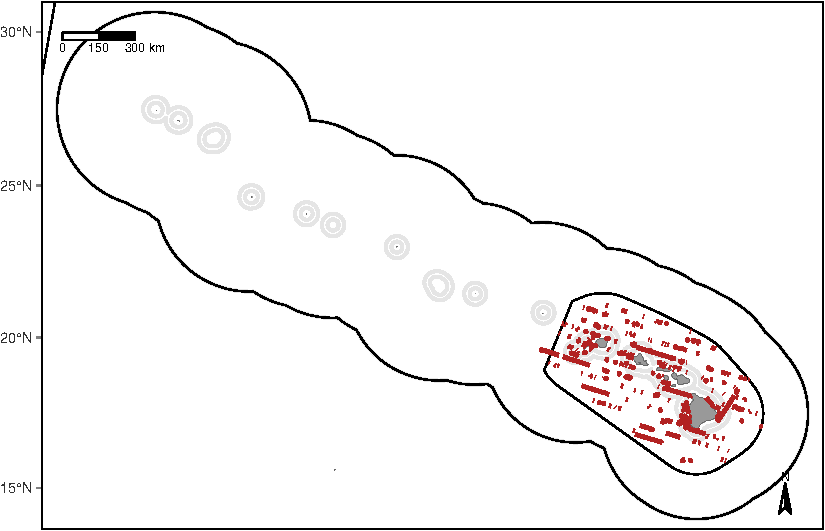
\includegraphics{figures/unnamed-chunk-59-1.pdf}

\hypertarget{color-code-conditions}{%
\paragraph{Color-code conditions}\label{color-code-conditions}}
\addcontentsline{toc}{paragraph}{Color-code conditions}

Your second customization option is to add format variables to the \texttt{segments} slot of the cohort of interest in the \texttt{cruz} object. This gives you full control of line color, thickness, and line-type according to whatever specifications you wish to set, e.g., color-coding by effort type or Beaufort sea state.

This is possible because the function \texttt{map\_effort()} looks for the variables \texttt{col} (line color), \texttt{lwd} (line thickness or stroke), and \texttt{lty} (line type) in the columns of \texttt{cruz\$segments}. If these columns exist, the values therein will be used instead of the function defaults.

For example, color-code by Beaufort scale:

\begin{Shaded}
\begin{Highlighting}[]
\CommentTok{# Save copy of cruz object data to modify}
\NormalTok{cruz2 <-}\StringTok{ }\NormalTok{cruz}
\NormalTok{segments <-}\StringTok{ }\NormalTok{cruz2}\OperatorTok{$}\NormalTok{cohorts}\OperatorTok{$}\NormalTok{default}\OperatorTok{$}\NormalTok{density}\OperatorTok{$}\NormalTok{segments}

\CommentTok{# Add column `col`: color code by BFT sea state}
\NormalTok{bft_colors <-}\StringTok{ }\KeywordTok{c}\NormalTok{(}\StringTok{'steelblue4'}\NormalTok{,}\StringTok{'steelblue2'}\NormalTok{,}\StringTok{'cadetblue1'}\NormalTok{,}\StringTok{'grey'}\NormalTok{)}
\NormalTok{segments}\OperatorTok{$}\NormalTok{col <-}\StringTok{ }\NormalTok{bft_colors[}\DecValTok{4}\NormalTok{]}
\NormalTok{segments}\OperatorTok{$}\NormalTok{col[ segments}\OperatorTok{$}\NormalTok{avgBft }\OperatorTok{<=}\StringTok{ }\DecValTok{7}\NormalTok{ ] <-}\StringTok{ }\NormalTok{bft_colors[}\DecValTok{3}\NormalTok{] }\CommentTok{# bft 5 +}
\NormalTok{segments}\OperatorTok{$}\NormalTok{col[ segments}\OperatorTok{$}\NormalTok{avgBft }\OperatorTok{<=}\StringTok{ }\DecValTok{4}\NormalTok{ ] <-}\StringTok{ }\NormalTok{bft_colors[}\DecValTok{2}\NormalTok{] }\CommentTok{# bft 3 - 4}
\NormalTok{segments}\OperatorTok{$}\NormalTok{col[ segments}\OperatorTok{$}\NormalTok{avgBft }\OperatorTok{<=}\StringTok{ }\DecValTok{2}\NormalTok{ ] <-}\StringTok{ }\NormalTok{bft_colors[}\DecValTok{1}\NormalTok{] }\CommentTok{# bft 0 -2}

\CommentTok{# Update sub_segments slot in `cruz` object}
\NormalTok{cruz2}\OperatorTok{$}\NormalTok{cohorts}\OperatorTok{$}\NormalTok{default}\OperatorTok{$}\NormalTok{density}\OperatorTok{$}\NormalTok{segments <-}\StringTok{ }\NormalTok{segments}

\CommentTok{# Update map }
\NormalTok{m_custom2 <-}\StringTok{ }\KeywordTok{map_effort}\NormalTok{(m, cruz2)}

\CommentTok{# Add legend using native functions from mapping package `tmap`}
\NormalTok{m_custom2 <-}\StringTok{ }
\StringTok{  }\NormalTok{m_custom2 }\OperatorTok{+}\StringTok{ }
\StringTok{  }\NormalTok{tmap}\OperatorTok{::}\KeywordTok{tm_add_legend}\NormalTok{(}\StringTok{'line'}\NormalTok{, }
                        \DataTypeTok{col =}\NormalTok{ bft_colors,}
                        \DataTypeTok{lwd =} \DecValTok{3}\NormalTok{,}
                        \DataTypeTok{labels =} \KeywordTok{c}\NormalTok{(}\StringTok{' 0 - 2'}\NormalTok{, }
                                   \StringTok{' 3 - 4'}\NormalTok{, }
                                   \StringTok{' 5 +'}\NormalTok{, }
                                   \StringTok{' no data'}\NormalTok{),}
                         \DataTypeTok{title=}\StringTok{"Beaufort sea state"}\NormalTok{) }\OperatorTok{+}
\StringTok{  }\NormalTok{tmap}\OperatorTok{::}\KeywordTok{tm_layout}\NormalTok{(}\DataTypeTok{legend.position=}\KeywordTok{c}\NormalTok{(}\StringTok{'left'}\NormalTok{,}\StringTok{'bottom'}\NormalTok{))}

\CommentTok{# Show map}
\NormalTok{m_custom2}
\end{Highlighting}
\end{Shaded}

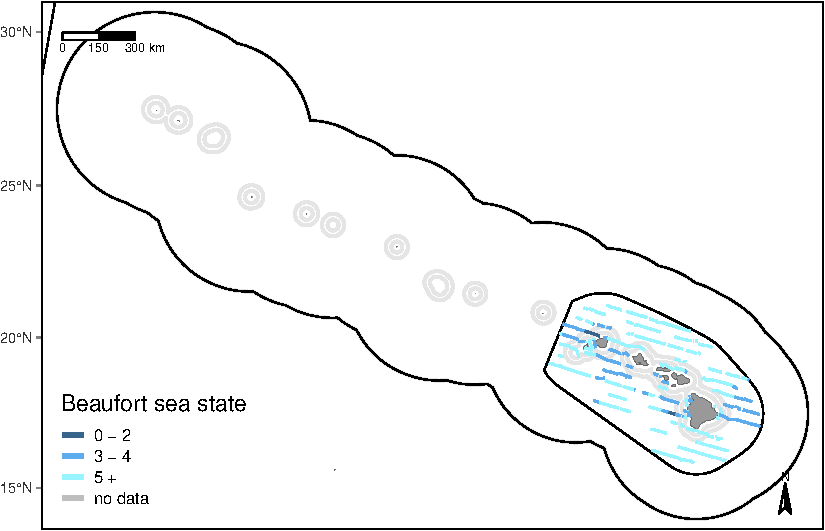
\includegraphics{figures/unnamed-chunk-60-1.pdf}

\hypertarget{add-sightings}{%
\subsection*{Add sightings}\label{add-sightings}}
\addcontentsline{toc}{subsection}{Add sightings}

Use the function \texttt{map\_sightings()} to add sightings to your map:

\begin{Shaded}
\begin{Highlighting}[]
\KeywordTok{map_sightings}\NormalTok{(m, cruz)}
\end{Highlighting}
\end{Shaded}

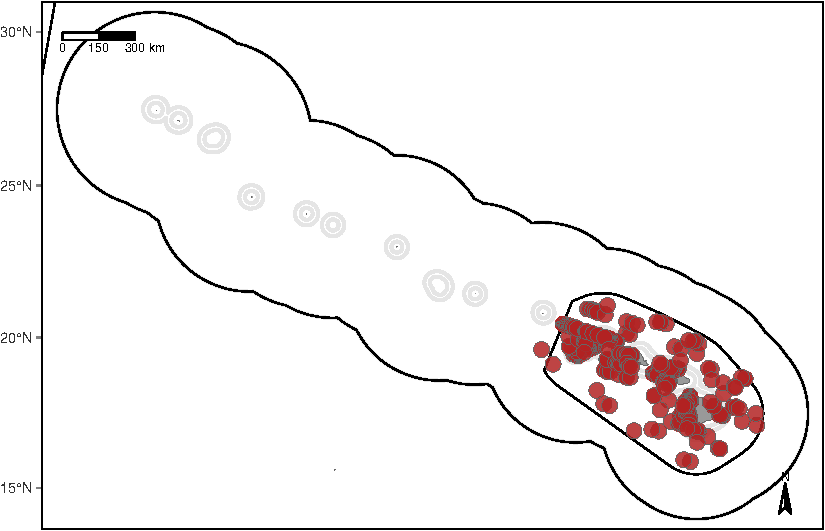
\includegraphics{figures/unnamed-chunk-61-1.pdf}

\hypertarget{customizing-sightings}{%
\subsubsection*{Customizing sightings}\label{customizing-sightings}}
\addcontentsline{toc}{subsubsection}{Customizing sightings}

To demonstrate some of the customization options, consider this map that shows sightings of false killer whales with custom dot color, shape, and size:

\begin{Shaded}
\begin{Highlighting}[]
\KeywordTok{map_sightings}\NormalTok{(m,}
\NormalTok{              cruz,}
              \DataTypeTok{include_species =} \StringTok{'033'}\NormalTok{,}
              \DataTypeTok{color_base =} \StringTok{'purple'}\NormalTok{,}
              \DataTypeTok{shape_base =} \DecValTok{18}\NormalTok{,}
              \DataTypeTok{size_base =} \DecValTok{1}\NormalTok{)}
\end{Highlighting}
\end{Shaded}

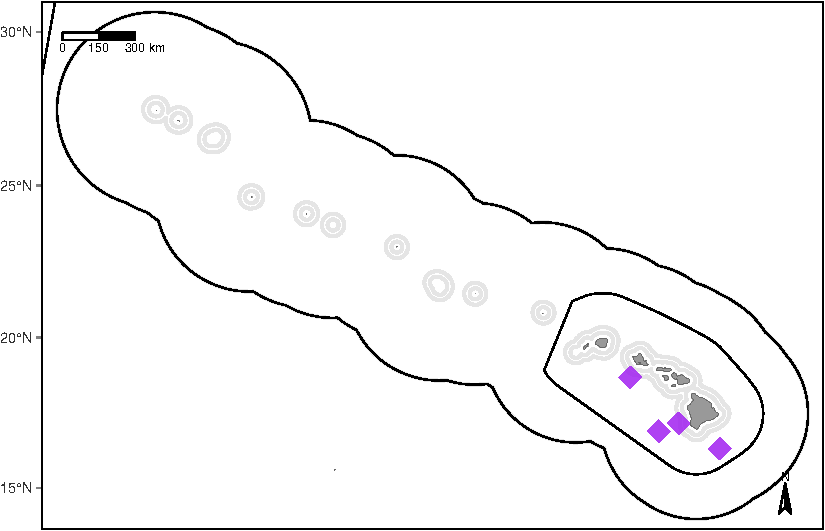
\includegraphics{figures/unnamed-chunk-62-1.pdf}

Next is a map of humpback whales and sperm whales, color-coded by species and shape-coded by whether or not the sighting will be included in the analysis:

\begin{Shaded}
\begin{Highlighting}[]
\KeywordTok{map_sightings}\NormalTok{(m, }
\NormalTok{              cruz,}
              \DataTypeTok{include_species =} \KeywordTok{c}\NormalTok{(}\StringTok{'076'}\NormalTok{,}\StringTok{'046'}\NormalTok{),}
              \DataTypeTok{color_code =} \OtherTok{TRUE}\NormalTok{,}
              \DataTypeTok{shape_code =} \OtherTok{TRUE}\NormalTok{)}
\end{Highlighting}
\end{Shaded}

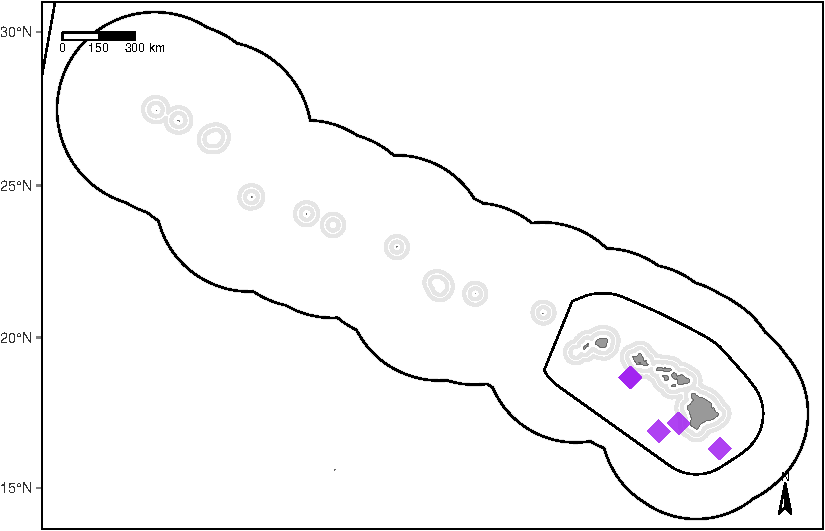
\includegraphics{figures/unnamed-chunk-63-1.pdf}

\hypertarget{overview}{%
\subsection*{Overview}\label{overview}}
\addcontentsline{toc}{subsection}{Overview}

Here is an overview of the steps needed to map strata, survey tracks, and sightings all together:

\begin{Shaded}
\begin{Highlighting}[]
\NormalTok{m <-}\StringTok{ }\KeywordTok{map_base}\NormalTok{(}\StringTok{'cnp'}\NormalTok{) }
\NormalTok{m <-}\StringTok{ }\KeywordTok{map_strata}\NormalTok{(m, cruz}\OperatorTok{$}\NormalTok{settings)}
\NormalTok{m <-}\StringTok{ }\KeywordTok{map_effort}\NormalTok{(m, cruz)}
\NormalTok{m <-}\StringTok{ }\KeywordTok{map_sightings}\NormalTok{(m, cruz, }\DataTypeTok{size_base=}\NormalTok{.}\DecValTok{4}\NormalTok{)}
\NormalTok{m }
\end{Highlighting}
\end{Shaded}

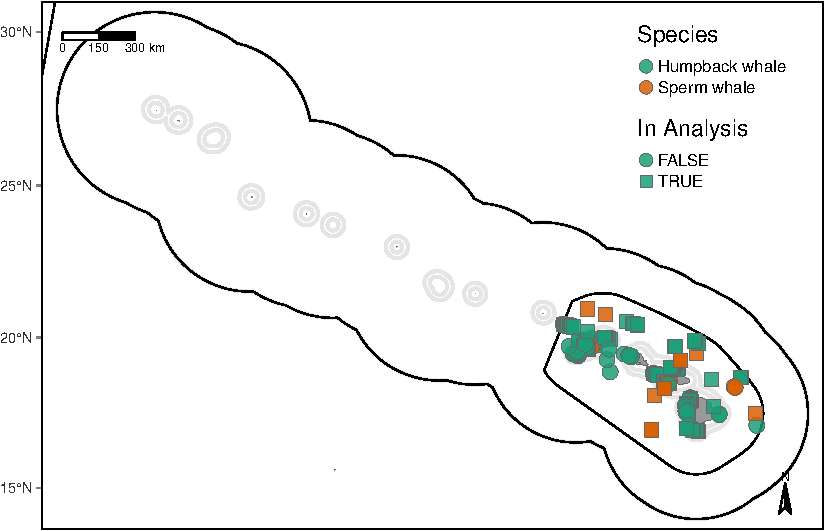
\includegraphics{figures/unnamed-chunk-64-1.pdf}

\hypertarget{interactive-maps}{%
\section*{Interactive maps}\label{interactive-maps}}
\addcontentsline{toc}{section}{Interactive maps}

\texttt{LTabundR} also has an interactive map function, which maps survey data using the \texttt{leaflet} package.

\begin{Shaded}
\begin{Highlighting}[]
 \KeywordTok{map_cruz}\NormalTok{(cruz,}
          \DataTypeTok{cohort=}\DecValTok{1}\NormalTok{,}
          \DataTypeTok{analysis=}\StringTok{'density'}\NormalTok{,}
          \DataTypeTok{eez_show=}\OtherTok{FALSE}\NormalTok{,}
          \DataTypeTok{strata_show=}\OtherTok{FALSE}\NormalTok{,}
          \DataTypeTok{effort_show=}\OtherTok{TRUE}\NormalTok{,}
          \DataTypeTok{effort_resolution=}\DecValTok{1}\NormalTok{,}
          \DataTypeTok{sightings_show=}\OtherTok{TRUE}\NormalTok{,}
          \DataTypeTok{sightings_color =} \StringTok{'firebrick'}\NormalTok{,}
          \DataTypeTok{verbose=}\OtherTok{FALSE}\NormalTok{)}
\end{Highlighting}
\end{Shaded}

Note that you can also click on sightings and tracklines to see their details. Refer to the documentation for this function (\texttt{?map\_cruz}) to see all the options available for stylizing these maps.

\hypertarget{interactive-dashboard}{%
\section*{Interactive dashboard}\label{interactive-dashboard}}
\addcontentsline{toc}{section}{Interactive dashboard}

Finally, note that \texttt{LTabundR} comes with an interactive data explorer app (a \texttt{Shiny} app) for filtering survey data according to effort scenario and species code, toggling \texttt{map\_cruz()} settings, and reviewing summary tables of effort and sightings (including inspection of truncation distances).

\begin{Shaded}
\begin{Highlighting}[]
\KeywordTok{cruz_explorer}\NormalTok{(cruz)}
\end{Highlighting}
\end{Shaded}

\emph{Screenshots from this app:}

~\\

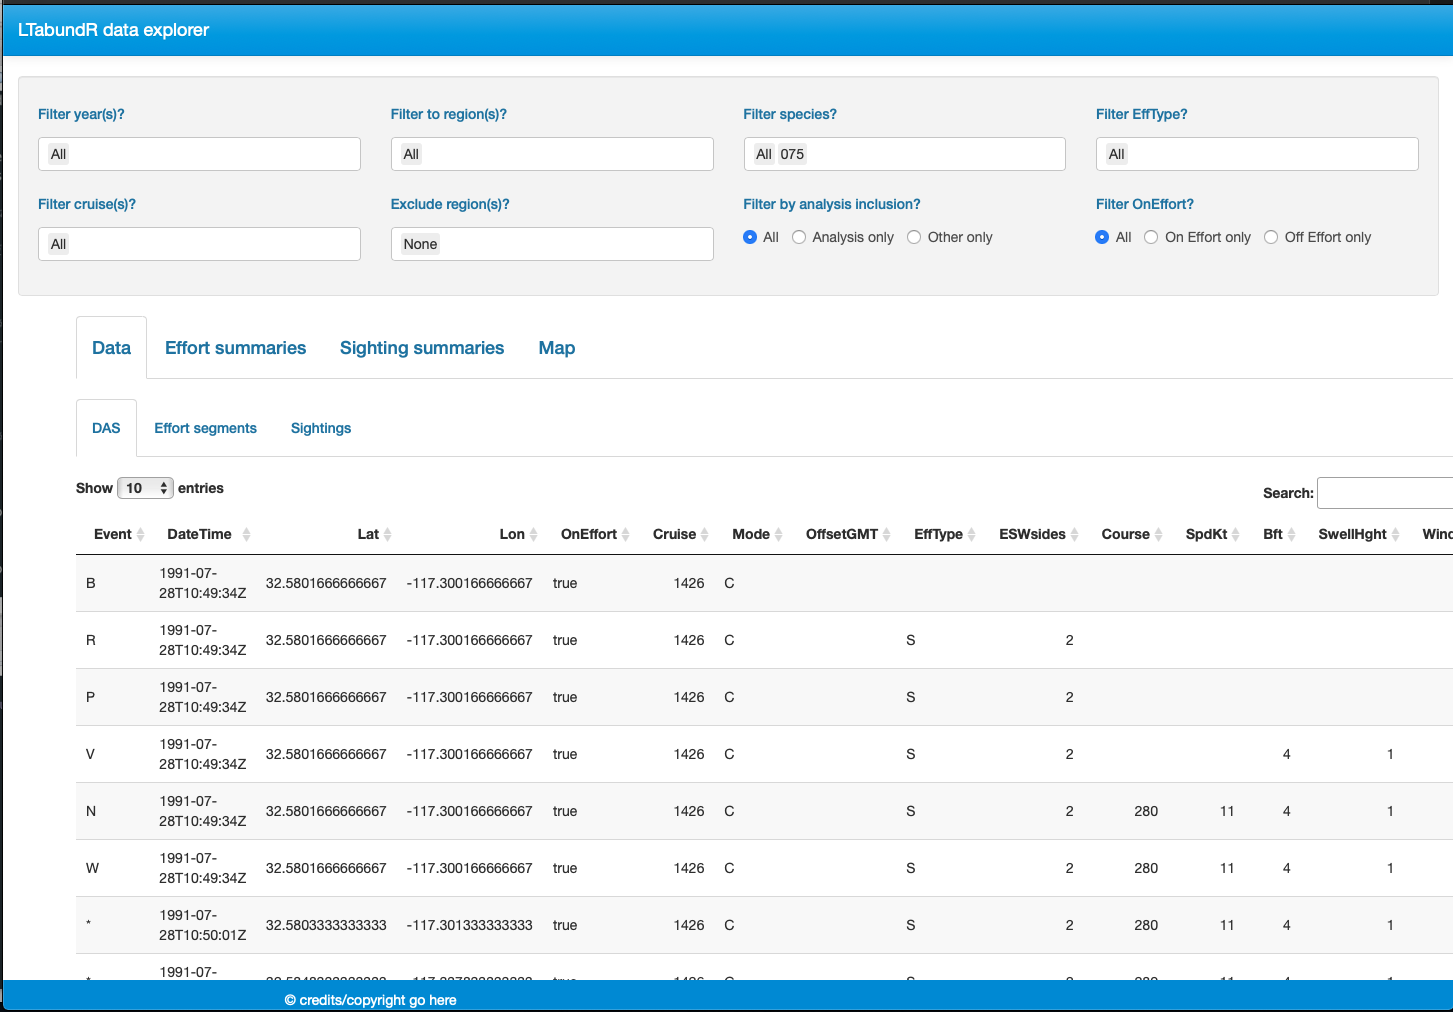
\includegraphics[width=0.85\textwidth,height=\textheight]{img/app-1.png}
~\\
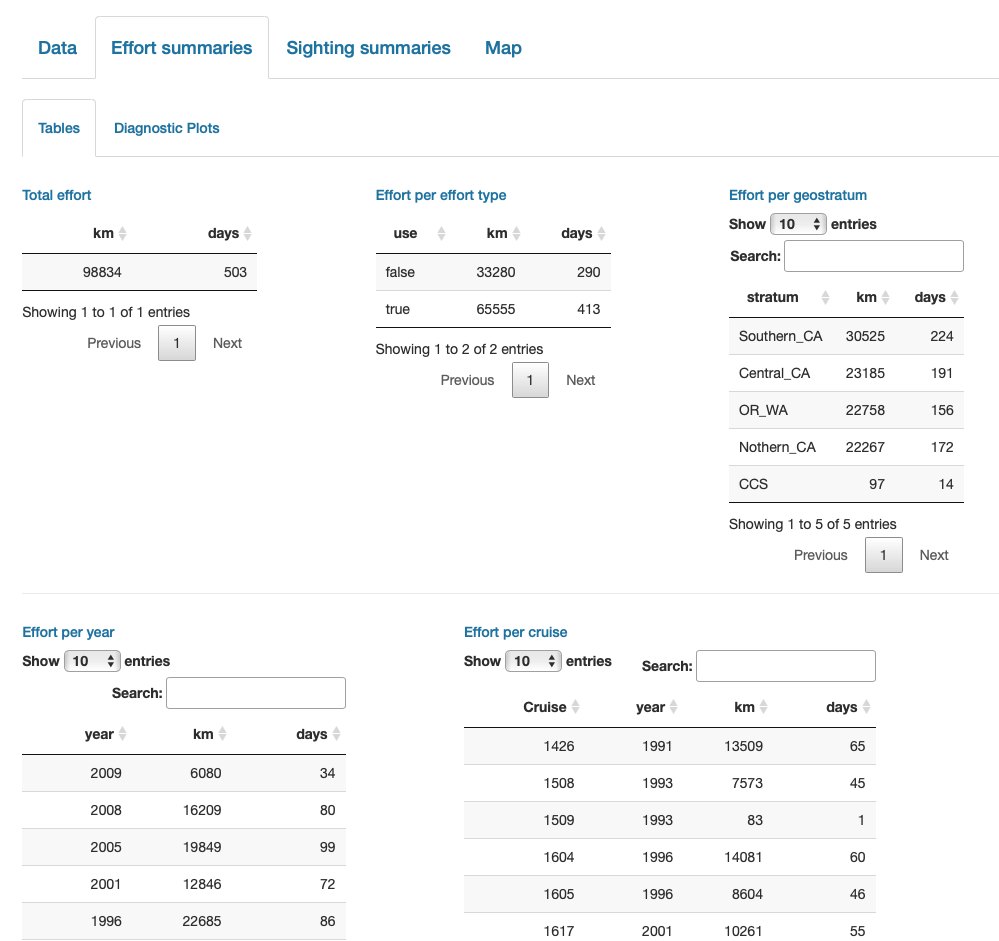
\includegraphics[width=0.85\textwidth,height=\textheight]{img/app-2.png}
~\\
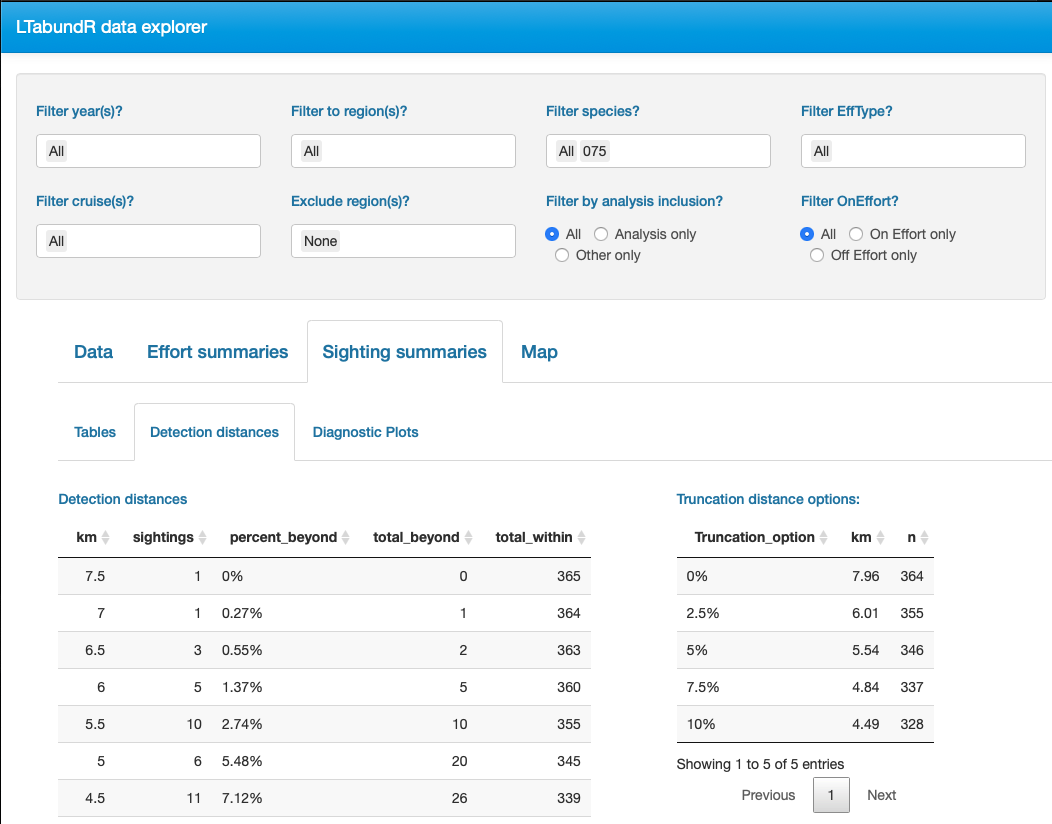
\includegraphics[width=0.85\textwidth,height=\textheight]{img/app-3.png}
~\\
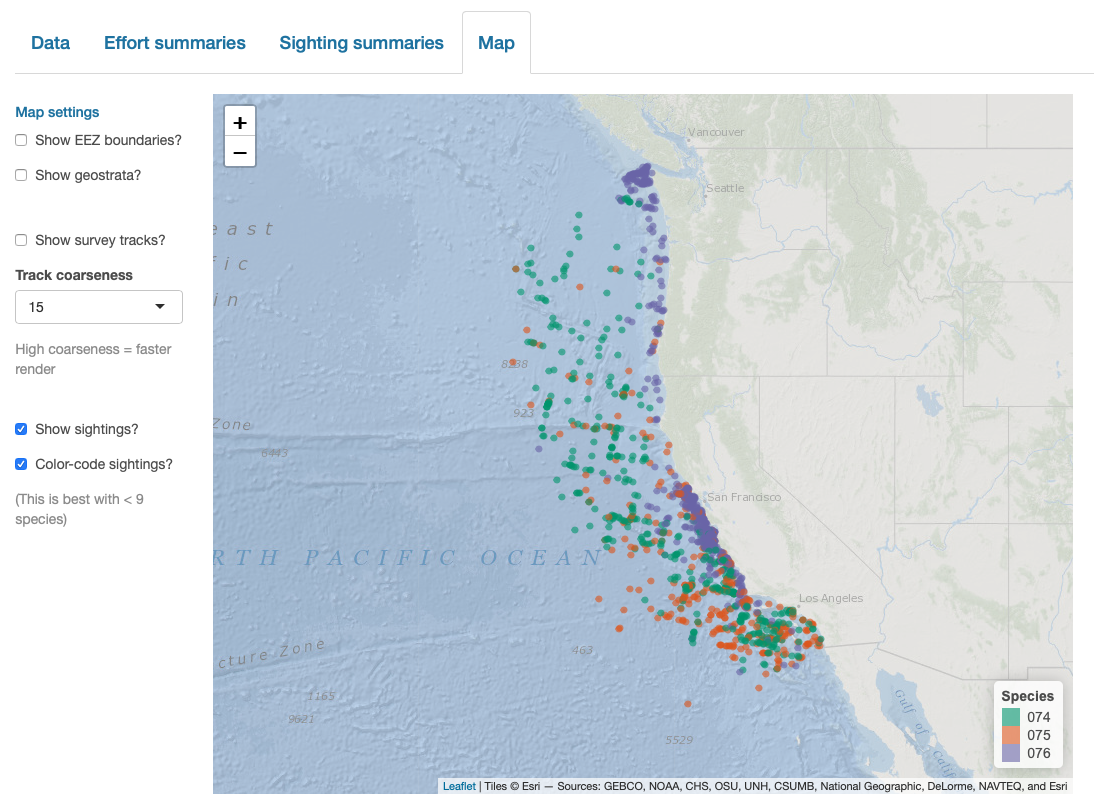
\includegraphics[width=0.85\textwidth,height=\textheight]{img/app-4.png}
~\\
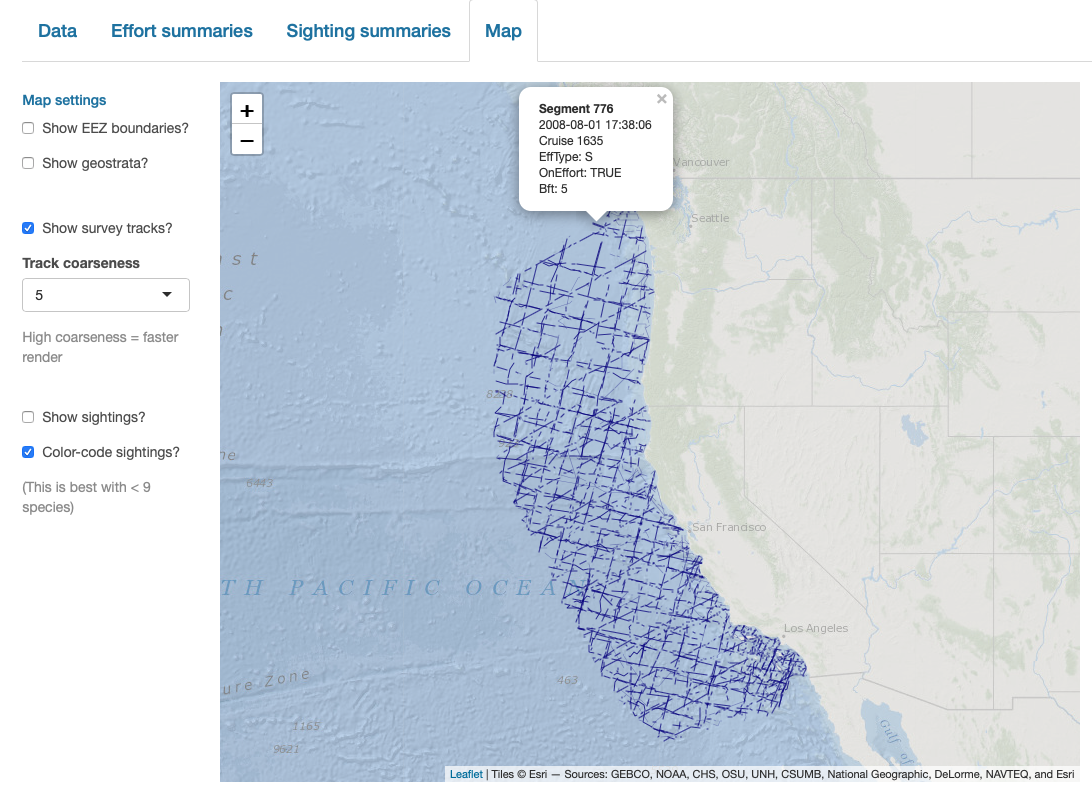
\includegraphics[width=0.85\textwidth,height=\textheight]{img/app-5.png}

\hypertarget{summarize}{%
\chapter{Summarize survey}\label{summarize}}

\hypertarget{summariz-effort}{%
\section*{Summariz effort}\label{summariz-effort}}
\addcontentsline{toc}{section}{Summariz effort}

The \texttt{summarize\_effort()} functions builds tables with total kilometers and days surveyed.

\begin{Shaded}
\begin{Highlighting}[]
\NormalTok{effort_summary <-}\StringTok{ }\KeywordTok{summarize_effort}\NormalTok{(cruz,}
                                      \DataTypeTok{cohort=}\DecValTok{1}\NormalTok{,}
                                      \DataTypeTok{analysis=}\StringTok{'density'}\NormalTok{)}
\end{Highlighting}
\end{Shaded}

This function summarizes effort in three default tables:

\begin{Shaded}
\begin{Highlighting}[]
\NormalTok{effort_summary }\OperatorTok\StringTok{  }\KeywordTok{names}\NormalTok{()}
\NormalTok{[}\DecValTok{1}\NormalTok{] }\StringTok{"total"}            \StringTok{"total_by_cruise"}  \StringTok{"total_by_year"}    \StringTok{"total_by_effort"} 
\NormalTok{[}\DecValTok{5}\NormalTok{] }\StringTok{"total_by_stratum"}
\end{Highlighting}
\end{Shaded}

\hypertarget{total-surveyed}{%
\subsection*{Total surveyed}\label{total-surveyed}}
\addcontentsline{toc}{subsection}{Total surveyed}

The slot \texttt{\$total} provides the grand total distance and days surveyed:

\begin{Shaded}
\begin{Highlighting}[]
\KeywordTok{library}\NormalTok{(DT)}

\NormalTok{effort_summary}\OperatorTok{$}\NormalTok{total }\OperatorTok\StringTok{ }
\StringTok{  }\NormalTok{DT}\OperatorTok{::}\KeywordTok{datatable}\NormalTok{(}\DataTypeTok{options=}\KeywordTok{list}\NormalTok{(}\DataTypeTok{initComplete =}\NormalTok{ htmlwidgets}\OperatorTok{::}\KeywordTok{JS}\NormalTok{(}
          \StringTok{"function(settings, json) \{$(this.api().table().container()).css(\{'font-size': '9pt'\});\}"}\NormalTok{)}
\NormalTok{       )) }
\end{Highlighting}
\end{Shaded}

\hypertarget{total-surveyed-by-effort}{%
\subsection*{Total surveyed by effort}\label{total-surveyed-by-effort}}
\addcontentsline{toc}{subsection}{Total surveyed by effort}

The slot \texttt{\$total\_by\_effort} provides the total distance and days surveyed, grouped by segments that will be included in the analysis and those that won't:

\hypertarget{total-surveyed-by-stratum}{%
\subsection*{Total surveyed by stratum}\label{total-surveyed-by-stratum}}
\addcontentsline{toc}{subsection}{Total surveyed by stratum}

The slot \texttt{\$total\_by\_stratum} provides the total distance and days surveyed within each stratum, again grouped by segments that will be included in the analysis and those that won't:

\hypertarget{summarize-sightings}{%
\section*{Summarize sightings}\label{summarize-sightings}}
\addcontentsline{toc}{section}{Summarize sightings}

The \texttt{summarize\_sightings()} function builds tables summarizing the sightings within each cohort-analysis. (Eventually, we may want to include an option to merge all sightings from all cohort-analyses into a single table.)

\begin{Shaded}
\begin{Highlighting}[]
\NormalTok{sightings_summary <-}\StringTok{ }\KeywordTok{summarize_sightings}\NormalTok{(cruz,}
                                         \DataTypeTok{cohort=}\DecValTok{1}\NormalTok{,}
                                         \DataTypeTok{analysis=}\StringTok{'density'}\NormalTok{)}
\end{Highlighting}
\end{Shaded}

This function summarizes sightings in four default tables:

\begin{Shaded}
\begin{Highlighting}[]
\NormalTok{sightings_summary }\OperatorTok\StringTok{  }\KeywordTok{names}\NormalTok{()}
\NormalTok{[}\DecValTok{1}\NormalTok{] }\StringTok{"simple_totals"}           \StringTok{"analysis_totals"}        
\NormalTok{[}\DecValTok{3}\NormalTok{] }\StringTok{"stratum_simple_totals"}   \StringTok{"stratum_analysis_totals"}
\end{Highlighting}
\end{Shaded}

\hypertarget{simple-species-totals}{%
\subsection*{Simple species totals}\label{simple-species-totals}}
\addcontentsline{toc}{subsection}{Simple species totals}

The slot \texttt{\$simple\_totals} includes all sightings, even if they will not be inluded in analysis:

\hypertarget{analysis-totals}{%
\subsection*{Analysis totals}\label{analysis-totals}}
\addcontentsline{toc}{subsection}{Analysis totals}

The slot \texttt{\$analysis\_totals} only includes sightings that meet all inclusion criteria for the analysis:

\hypertarget{simple-totals-for-each-stratum}{%
\subsection*{Simple totals for each stratum}\label{simple-totals-for-each-stratum}}
\addcontentsline{toc}{subsection}{Simple totals for each stratum}

The slot \texttt{\$stratum\_simple\_totals} splits the first table (simple species totals) so that sightings are tallied for each geo-stratum separately:

\hypertarget{analysis-totals-for-each-stratum}{%
\subsection*{Analysis totals for each stratum}\label{analysis-totals-for-each-stratum}}
\addcontentsline{toc}{subsection}{Analysis totals for each stratum}

The slot \texttt{\$stratum\_analysis\_totals} splits the second table (analysis totals for each species) so that sightings are tallied for each geo-stratum separately:

\hypertarget{df}{%
\chapter{Detection functions}\label{df}}

\hypertarget{format-for-distance}{%
\section*{\texorpdfstring{Format for \texttt{Distance}}{Format for Distance}}\label{format-for-distance}}
\addcontentsline{toc}{section}{Format for \texttt{Distance}}

To format the processed data for use in \texttt{Distance}-related analyses, use the function \texttt{format\_distance()}.

\begin{Shaded}
\begin{Highlighting}[]
\NormalTok{cruz_dist <-}\StringTok{ }\KeywordTok{format_distance}\NormalTok{(cruz,}
                             \DataTypeTok{cohort=}\DecValTok{1}\NormalTok{,}
                             \DataTypeTok{analysis=}\StringTok{'density'}\NormalTok{)}
\end{Highlighting}
\end{Shaded}

This function produces a list with four slots:

\begin{Shaded}
\begin{Highlighting}[]
\NormalTok{cruz_dist }\OperatorTok\StringTok{  }\NormalTok{names}
\NormalTok{[}\DecValTok{1}\NormalTok{] }\StringTok{"cohort"}    \StringTok{"analysis"}  \StringTok{"effort"}    \StringTok{"sightings"}
\end{Highlighting}
\end{Shaded}

The first two slots specify which cohort and analysis these data pertain to.

The second two slots, \texttt{effort} and \texttt{sightings}, mirror the format of the \texttt{EFFORT.csv} and \texttt{SIGHTINGS.csv} files produced by \texttt{ABUND\ 7/9}:

\hypertarget{effort}{%
\subsection*{Effort}\label{effort}}
\addcontentsline{toc}{subsection}{Effort}

\hypertarget{sightings}{%
\subsection*{Sightings}\label{sightings}}
\addcontentsline{toc}{subsection}{Sightings}

\hypertarget{abundance}{%
\chapter{Abundance estimation}\label{abundance}}

\emph{Coming soon!}

\hypertarget{part-case-studies}{%
\part{Case studies}\label{part-case-studies}}

\hypertarget{casestudies}{%
\chapter{Central North Pacific}\label{casestudies}}

To demonstrate what we are building, below is template for quickly running all of the steps detailed in subsequent chapters.

This template uses the same data and settings used throughout the vignette:

\begin{Shaded}
\begin{Highlighting}[]
\KeywordTok{library}\NormalTok{(swfscDAS)}
\KeywordTok{library}\NormalTok{(LTabundR)}
\KeywordTok{library}\NormalTok{(dplyr)}

\CommentTok{# Settings =====================================================================}

\CommentTok{# Load strata dataframes}
\KeywordTok{data}\NormalTok{(strata_cnp)}
\KeywordTok{data}\NormalTok{(study_cnp)}

\CommentTok{# Load group size coefficients}
\KeywordTok{data}\NormalTok{(group_size_coefficients)}

\CommentTok{# Load ships}
\KeywordTok{data}\NormalTok{(ships)}

\CommentTok{# Load species codes}
\KeywordTok{data}\NormalTok{(species_codes)}

\CommentTok{# Survey settings}
\NormalTok{survey <-}\StringTok{ }
\StringTok{  }\KeywordTok{load_survey_settings}\NormalTok{(}\DataTypeTok{out_handling =} \StringTok{'stratum'}\NormalTok{,}
                       \DataTypeTok{max_row_interval =} \DecValTok{700}\NormalTok{,}
                       \DataTypeTok{segment_method =} \StringTok{'equallength'}\NormalTok{,}
                       \DataTypeTok{segment_target_km =} \DecValTok{30}\NormalTok{,}
                       \DataTypeTok{segment_max_interval =} \DecValTok{48}\NormalTok{,}
                       \DataTypeTok{segment_type_handling =} \StringTok{'separate'}\NormalTok{,}
                       \DataTypeTok{segment_remainder_handling =} \KeywordTok{c}\NormalTok{(}\StringTok{'append'}\NormalTok{,}\StringTok{'segment'}\NormalTok{),}
                       \DataTypeTok{ship_list =}\NormalTok{ ships,}
                       \DataTypeTok{species_codes =}\NormalTok{ species_codes,}
                       \DataTypeTok{group_size_coefficients =}\NormalTok{ group_size_coefficients,}
                       \DataTypeTok{smear_angles =} \OtherTok{FALSE}\NormalTok{,}
                       \DataTypeTok{verbose =} \OtherTok{TRUE}\NormalTok{)}

\CommentTok{# Cohort 1 (default)}
\NormalTok{cohort1 <-}\StringTok{ }\KeywordTok{load_cohort_settings}\NormalTok{()}

\CommentTok{# Cohort 2}
\NormalTok{cohort2 <-}\StringTok{ }
\StringTok{  }\KeywordTok{load_cohort_settings}\NormalTok{(}\DataTypeTok{id=}\StringTok{'fkw_insular'}\NormalTok{,}
                       \DataTypeTok{species=}\DecValTok{33}\NormalTok{,}
                       \DataTypeTok{use_low_if_na =} \OtherTok{TRUE}\NormalTok{,}
                       \DataTypeTok{truncation_km =} \DecValTok{5}\NormalTok{,}
                       \DataTypeTok{strata_overlap_handling =} \StringTok{'each'}\NormalTok{)}

\CommentTok{# Finalize settings}
\NormalTok{settings <-}\StringTok{ }\KeywordTok{load_settings}\NormalTok{(}\DataTypeTok{strata =}\NormalTok{ strata_cnp,}
                          \DataTypeTok{study_area =}\NormalTok{ study_cnp,}
                          \DataTypeTok{survey =}\NormalTok{ survey,}
                          \DataTypeTok{cohorts=}\KeywordTok{list}\NormalTok{(cohort1,}
\NormalTok{                                       cohort2))}


\CommentTok{# Processing ===================================================================}

\CommentTok{# Load & format DAS}
\NormalTok{das_file <-}\StringTok{ 'data/surveys/HICEASwinter2020.das'}
\NormalTok{cruz <-}\StringTok{ }\KeywordTok{process_surveys}\NormalTok{(das_file, settings, }\DataTypeTok{verbose=}\OtherTok{TRUE}\NormalTok{)}

\CommentTok{# Review: segment length distribution}
\KeywordTok{hist}\NormalTok{(cruz}\OperatorTok{$}\NormalTok{cohorts}\OperatorTok{$}\NormalTok{default}\OperatorTok{$}\NormalTok{density}\OperatorTok{$}\NormalTok{segments}\OperatorTok{$}\NormalTok{dist,}
     \DataTypeTok{breaks =} \KeywordTok{seq}\NormalTok{(}\DecValTok{0}\NormalTok{,}\DecValTok{60}\NormalTok{,}\DataTypeTok{by=}\DecValTok{1}\NormalTok{),}
     \DataTypeTok{xlab=}\StringTok{'Segment lengths (km)'}\NormalTok{,}
     \DataTypeTok{main=}\KeywordTok{paste0}\NormalTok{(}\StringTok{'Target km: '}\NormalTok{,settings}\OperatorTok{$}\NormalTok{survey}\OperatorTok{$}\NormalTok{segment_target_km))}
\CommentTok{# Process sightings}
\NormalTok{cruz <-}\StringTok{ }\KeywordTok{process_sightings}\NormalTok{(cruz)}

\CommentTok{# Map}
\NormalTok{m <-}\StringTok{ }\KeywordTok{map_base}\NormalTok{(}\StringTok{'cnp'}\NormalTok{) }
\NormalTok{m <-}\StringTok{ }\KeywordTok{map_strata}\NormalTok{(m, cruz}\OperatorTok{$}\NormalTok{settings)}
\NormalTok{m <-}\StringTok{ }\KeywordTok{map_effort}\NormalTok{(m, cruz)}
\NormalTok{m <-}\StringTok{ }\KeywordTok{map_sightings}\NormalTok{(m, cruz, }\DataTypeTok{size_base=}\NormalTok{.}\DecValTok{4}\NormalTok{)}
\NormalTok{m }
\end{Highlighting}
\end{Shaded}

\hypertarget{california-current-system}{%
\chapter{California Current System}\label{california-current-system}}

\begin{Shaded}
\begin{Highlighting}[]
\KeywordTok{library}\NormalTok{(swfscDAS)}
\KeywordTok{library}\NormalTok{(LTabundR)}
\KeywordTok{library}\NormalTok{(dplyr)}

\CommentTok{# Settings =====================================================================}

\CommentTok{# Load strata & study area}
\KeywordTok{data}\NormalTok{(strata_ccs)}

\CommentTok{# Survey-wide}
\NormalTok{survey <-}\StringTok{ }
\StringTok{  }\KeywordTok{load_survey_settings}\NormalTok{(}\DataTypeTok{segment_method =} \StringTok{'equallength'}\NormalTok{,}
                       \DataTypeTok{segment_target_km =} \DecValTok{100}\NormalTok{,}
                       \DataTypeTok{segment_max_km_gap =} \DecValTok{5}\NormalTok{,}
                       \DataTypeTok{segment_max_interval =} \DecValTok{48}\NormalTok{,}
                       \DataTypeTok{segment_type_handling =} \StringTok{'separate'}\NormalTok{,}
                       \DataTypeTok{segment_remainder_handling =} \KeywordTok{c}\NormalTok{(}\StringTok{'append'}\NormalTok{,}\StringTok{'segment'}\NormalTok{),}
                       \DataTypeTok{verbose =} \OtherTok{TRUE}\NormalTok{)}

\CommentTok{# Cohort 1 (default)}
\NormalTok{cohort1 <-}\StringTok{ }\KeywordTok{load_cohort_settings}\NormalTok{()}

\CommentTok{# Cohort 2}
\NormalTok{cohort2 <-}\StringTok{ }
\StringTok{  }\KeywordTok{load_cohort_settings}\NormalTok{(}\DataTypeTok{id=}\StringTok{'beakers'}\NormalTok{,}
                       \DataTypeTok{species=}\KeywordTok{c}\NormalTok{(}\DecValTok{1}\NormalTok{,}\DecValTok{49}\NormalTok{,}\DecValTok{52}\OperatorTok{:}\DecValTok{59}\NormalTok{, }\DecValTok{61}\OperatorTok{:}\DecValTok{65}\NormalTok{, }\DecValTok{81}\OperatorTok{:}\DecValTok{83}\NormalTok{, }\DecValTok{106}\NormalTok{, }\DecValTok{109}\NormalTok{),}
                       \DataTypeTok{use_low_if_na =} \OtherTok{TRUE}\NormalTok{,}
                       \DataTypeTok{distance_types =} \KeywordTok{c}\NormalTok{(}\StringTok{'S'}\NormalTok{,}\StringTok{'F'}\NormalTok{,}\StringTok{'N'}\NormalTok{))}

\CommentTok{# Finalize settings}
\NormalTok{settings <-}\StringTok{ }\KeywordTok{load_settings}\NormalTok{(}\DataTypeTok{strata =}\NormalTok{ strata_ccs,}
                          \DataTypeTok{study_area =} \OtherTok{NULL}\NormalTok{,}
                          \DataTypeTok{survey =}\NormalTok{ survey,}
                          \DataTypeTok{cohorts=}\KeywordTok{list}\NormalTok{(cohort1,}
\NormalTok{                                       cohort2))}


\CommentTok{# Processing ===================================================================}

\CommentTok{# Load DAS & subset to a single cruise}
\NormalTok{das_file <-}\StringTok{ 'data/surveys/CAORWA_91-09.das'}
\NormalTok{das <-}\StringTok{ }\KeywordTok{load_das}\NormalTok{(das_file)}
\NormalTok{das <-}\StringTok{ }\NormalTok{das }\OperatorTok\StringTok{ }\KeywordTok{filter}\NormalTok{(Cruise }\OperatorTok{==}\StringTok{ }\DecValTok{1635}\NormalTok{)}

\CommentTok{# Format DAS data for LTabundR}
\NormalTok{das <-}\StringTok{ }\KeywordTok{format_das}\NormalTok{(das, settings)}

\CommentTok{# Process strata}
\NormalTok{cruz <-}\StringTok{ }\KeywordTok{process_strata}\NormalTok{(das, settings)}

\CommentTok{# Segmentize}
\NormalTok{cruz <-}\StringTok{ }\KeywordTok{segmentize}\NormalTok{(cruz, }\DataTypeTok{verbose=}\OtherTok{TRUE}\NormalTok{)}

\CommentTok{# Review: segment length distribution}
\NormalTok{kms <-}\StringTok{ }\NormalTok{cruz}\OperatorTok{$}\NormalTok{cohorts}\OperatorTok{$}\NormalTok{default}\OperatorTok{$}\NormalTok{density}\OperatorTok{$}\NormalTok{segments}\OperatorTok{$}\NormalTok{dist }
\KeywordTok{hist}\NormalTok{(kms,}
     \DataTypeTok{breaks =} \KeywordTok{seq}\NormalTok{(}\DecValTok{0}\NormalTok{,}\FloatTok{1.1}\OperatorTok{*}\KeywordTok{max}\NormalTok{(kms),}\DataTypeTok{by=}\DecValTok{1}\NormalTok{),}
     \DataTypeTok{xlab=}\StringTok{'Segment lengths (km)'}\NormalTok{,}
     \DataTypeTok{main=}\KeywordTok{paste0}\NormalTok{(}\StringTok{'Target km: '}\NormalTok{,settings}\OperatorTok{$}\NormalTok{survey}\OperatorTok{$}\NormalTok{segment_target_km))}

\CommentTok{# Process sightings}
\NormalTok{cruz <-}\StringTok{ }\KeywordTok{process_sightings}\NormalTok{(cruz)}

\CommentTok{# Map}
\NormalTok{m <-}\StringTok{ }\KeywordTok{map_base}\NormalTok{(}\StringTok{'ccs'}\NormalTok{) }
\NormalTok{m <-}\StringTok{ }\KeywordTok{map_strata}\NormalTok{(m, cruz}\OperatorTok{$}\NormalTok{settings)}
\NormalTok{m <-}\StringTok{ }\KeywordTok{map_effort}\NormalTok{(m, cruz)}
\NormalTok{m <-}\StringTok{ }\KeywordTok{map_sightings}\NormalTok{(m, cruz, }\DataTypeTok{size_base=}\NormalTok{.}\DecValTok{4}\NormalTok{)}
\NormalTok{m }
\end{Highlighting}
\end{Shaded}

\hypertarget{eastern-tropical-pacific}{%
\chapter{Eastern Tropical Pacific}\label{eastern-tropical-pacific}}

\emph{Coming soon!}

\hypertarget{practicalities}{%
\chapter{Practicalities}\label{practicalities}}

\hypertarget{reproducibility-project-management}{%
\subsection*{Reproducibility \& project management}\label{reproducibility-project-management}}
\addcontentsline{toc}{subsection}{Reproducibility \& project management}

One of the features of the \texttt{ABUND} framework we need to retain is that each analysis is self-contained and reproducible. The folder for an analysis must have all the files and data needed for someone else to be able to replicate it.

In the \texttt{R} package framework we are developing, the contents of a project folder will be straightforward (once the code base is bundled into a package).

\emph{Contents of a project folder:}

\begin{itemize}
\tightlist
\item
  \texttt{DAS} file(s) with survey data\\
\item
  Stratum and study area polygon(s), as \texttt{csv}(s) (optional)\\
\item
  Group size calibration files (optional)\\
\item
  An \texttt{analysis.R} file (or perhaps a \texttt{.Rmd}), containing an adaptation of the code provided in the template above. This script will contain project-specific settings (e.g., the \texttt{load\_settings()} call), which allow for the script to be reproducible.
\end{itemize}

\hypertarget{part-appendix}{%
\part{Appendix}\label{part-appendix}}

\hypertarget{stratagallery}{%
\chapter{Strata gallery}\label{stratagallery}}

This packages comes with several built-in datasets of geographic strata that are commonly used in NOAA/NMFS surveys. The functions \texttt{strata\_explore()} and \texttt{strata\_select()} were developed to help you explore those built-in options.

\hypertarget{central-north-pacific}{%
\section*{Central North Pacific}\label{central-north-pacific}}
\addcontentsline{toc}{section}{Central North Pacific}

\begin{Shaded}
\begin{Highlighting}[]
\KeywordTok{strata_explore}\NormalTok{(}\StringTok{'cnp'}\NormalTok{)}
\end{Highlighting}
\end{Shaded}

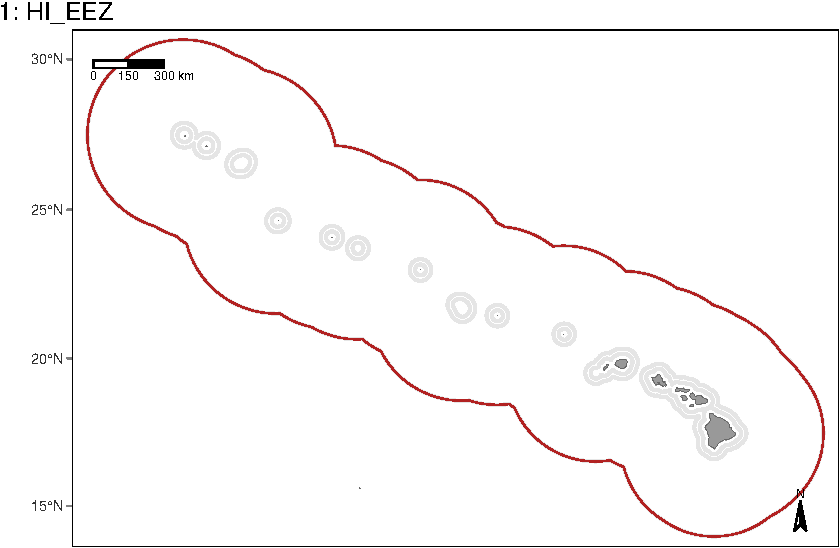
\includegraphics{figures/unnamed-chunk-87-1.pdf} 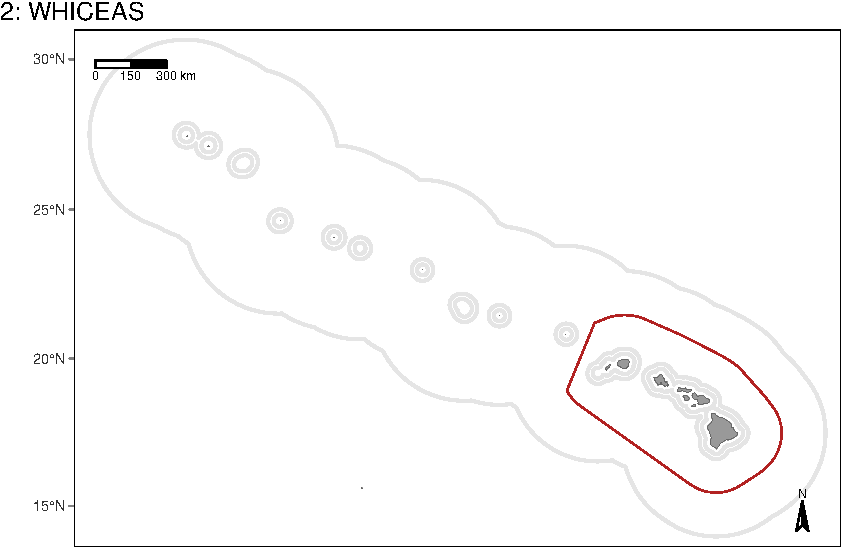
\includegraphics{figures/unnamed-chunk-87-2.pdf} 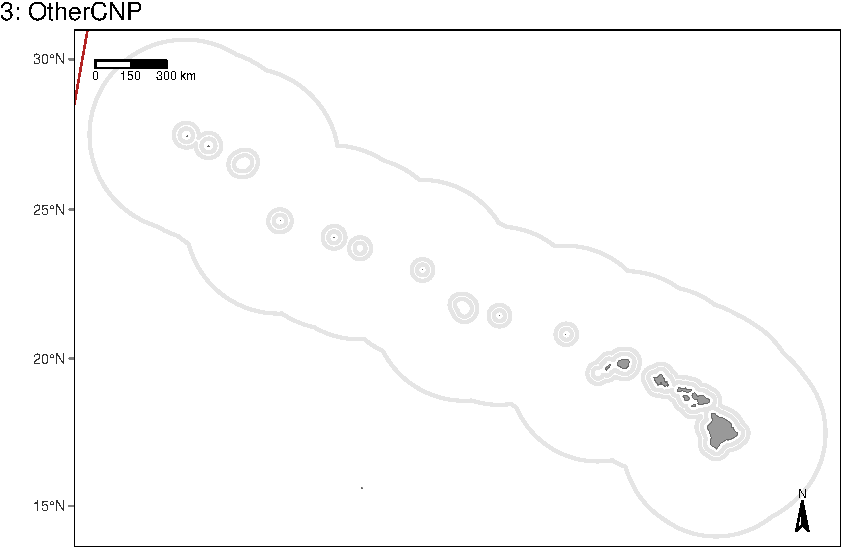
\includegraphics{figures/unnamed-chunk-87-3.pdf}

To acquire the filepath to one of these strata, pass the index (or indices) printed in the map titles above to the function \texttt{strata\_select()}:

\begin{Shaded}
\begin{Highlighting}[]
\NormalTok{strata <-}\StringTok{ }\KeywordTok{strata_select}\NormalTok{(}\DataTypeTok{selections =} \KeywordTok{c}\NormalTok{(}\DecValTok{1}\NormalTok{,}\DecValTok{3}\NormalTok{),}
                              \DataTypeTok{region =} \StringTok{'cnp'}\NormalTok{)}
\end{Highlighting}
\end{Shaded}

This function returns a named list that can be passed directly to the \texttt{strata} argument in \texttt{load\_settings()}.

\begin{Shaded}
\begin{Highlighting}[]
\NormalTok{strata }\OperatorTok\StringTok{ }\NormalTok{names}
\NormalTok{[}\DecValTok{1}\NormalTok{] }\StringTok{"HI_EEZ"}   \StringTok{"OtherCNP"}
\end{Highlighting}
\end{Shaded}

The second slot, \texttt{\$paths}, contains the filepaths you would need to pass to the \texttt{load\_settings()} function.

\hypertarget{california-current}{%
\section*{California Current}\label{california-current}}
\addcontentsline{toc}{section}{California Current}

\begin{Shaded}
\begin{Highlighting}[]
\KeywordTok{strata_explore}\NormalTok{(}\StringTok{'ccs'}\NormalTok{)}
\end{Highlighting}
\end{Shaded}

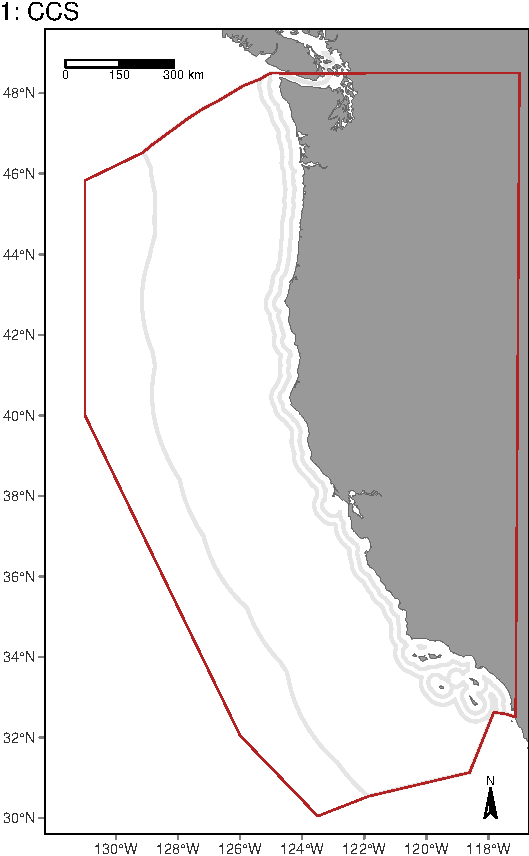
\includegraphics{figures/unnamed-chunk-90-1.pdf} 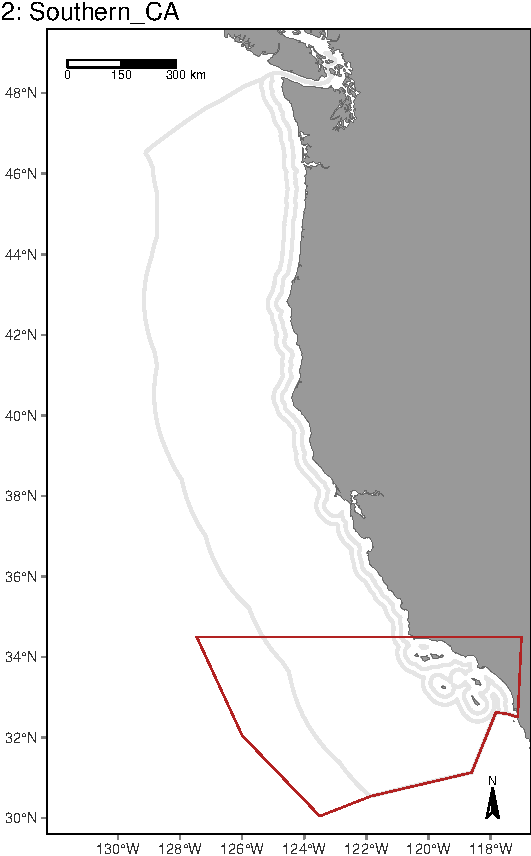
\includegraphics{figures/unnamed-chunk-90-2.pdf} 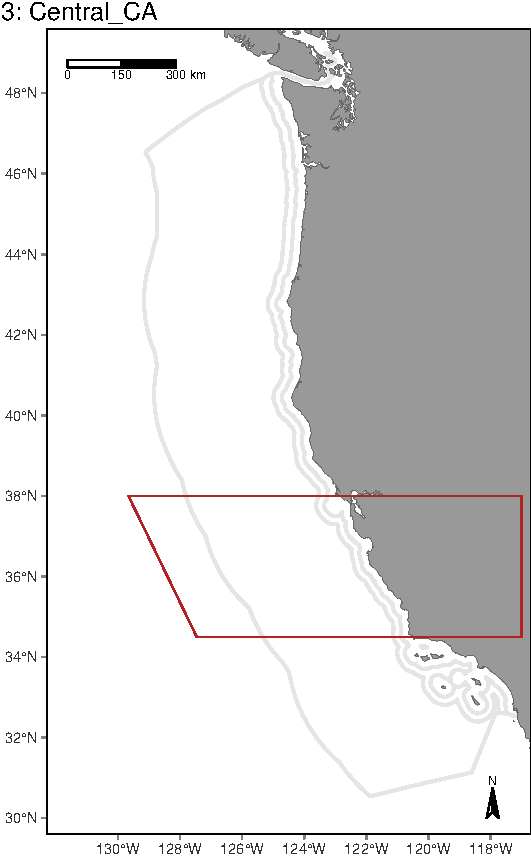
\includegraphics{figures/unnamed-chunk-90-3.pdf} 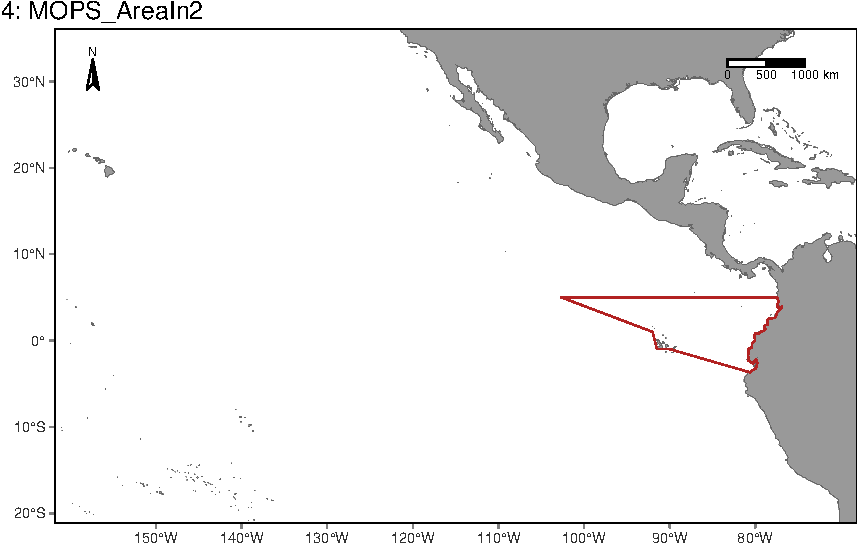
\includegraphics{figures/unnamed-chunk-90-4.pdf} 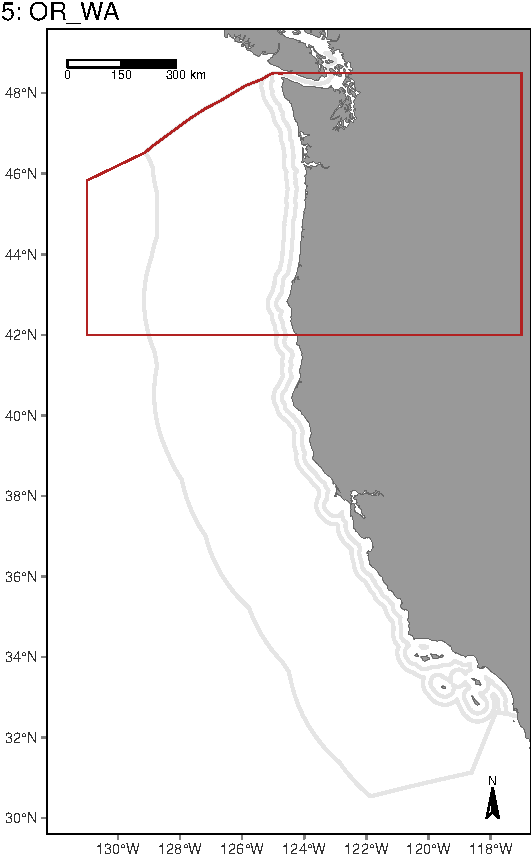
\includegraphics{figures/unnamed-chunk-90-5.pdf}

\hypertarget{etp}{%
\section*{ETP}\label{etp}}
\addcontentsline{toc}{section}{ETP}

\begin{Shaded}
\begin{Highlighting}[]
\KeywordTok{strata_explore}\NormalTok{(}\StringTok{'etp'}\NormalTok{)}
\end{Highlighting}
\end{Shaded}

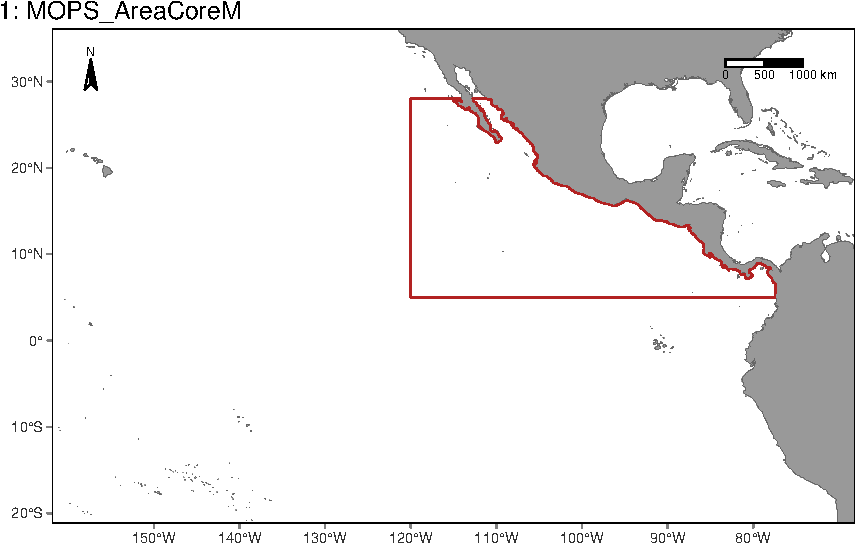
\includegraphics{figures/unnamed-chunk-91-1.pdf} 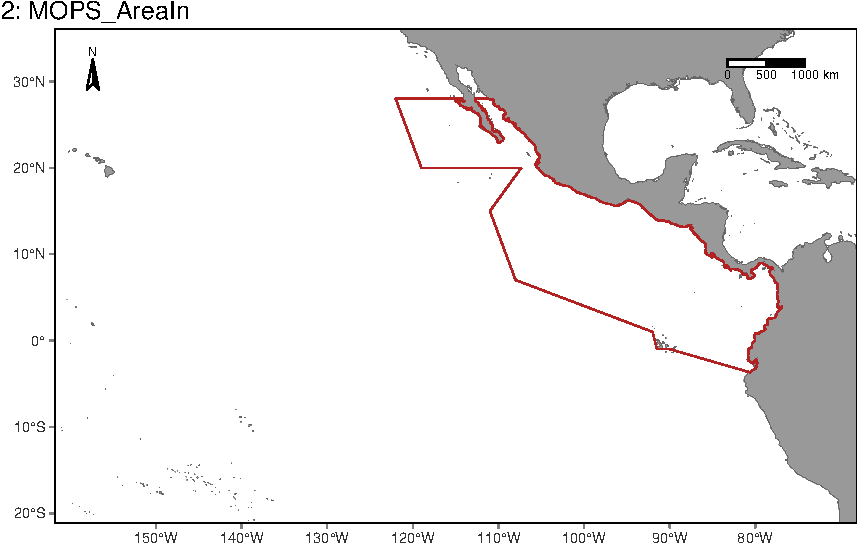
\includegraphics{figures/unnamed-chunk-91-2.pdf} 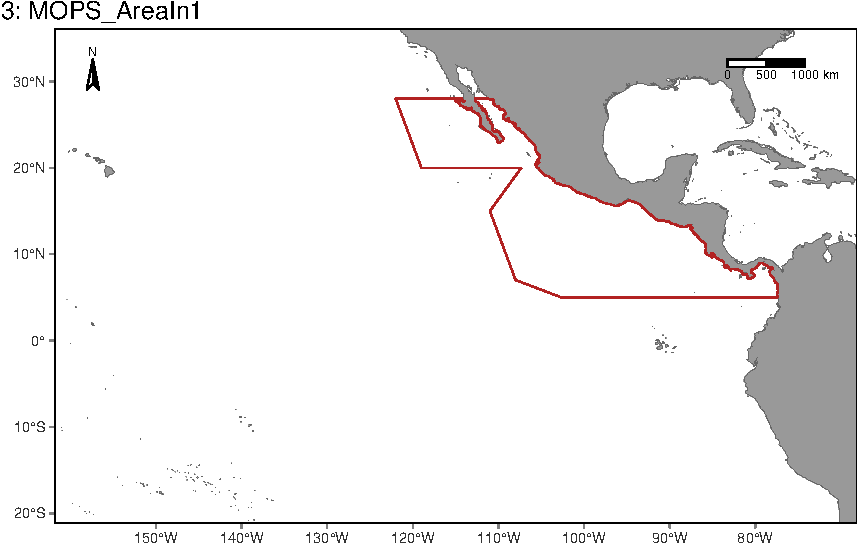
\includegraphics{figures/unnamed-chunk-91-3.pdf} 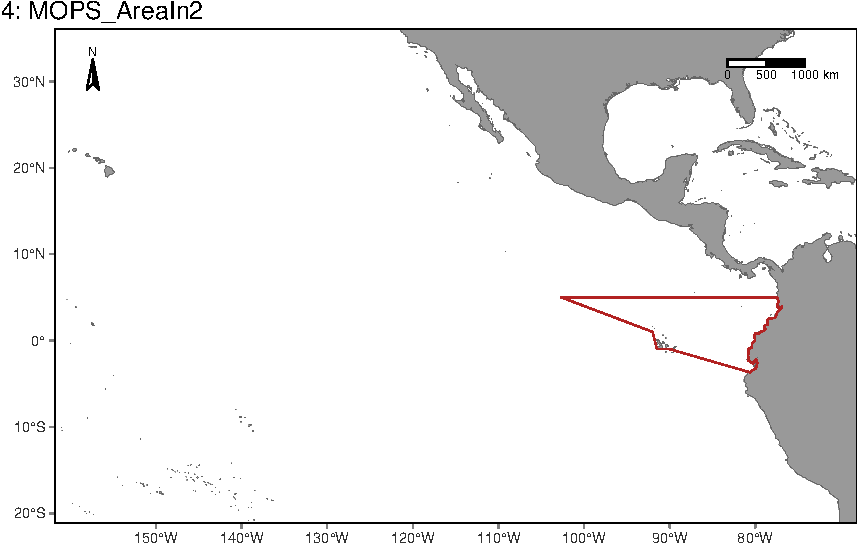
\includegraphics{figures/unnamed-chunk-91-4.pdf} 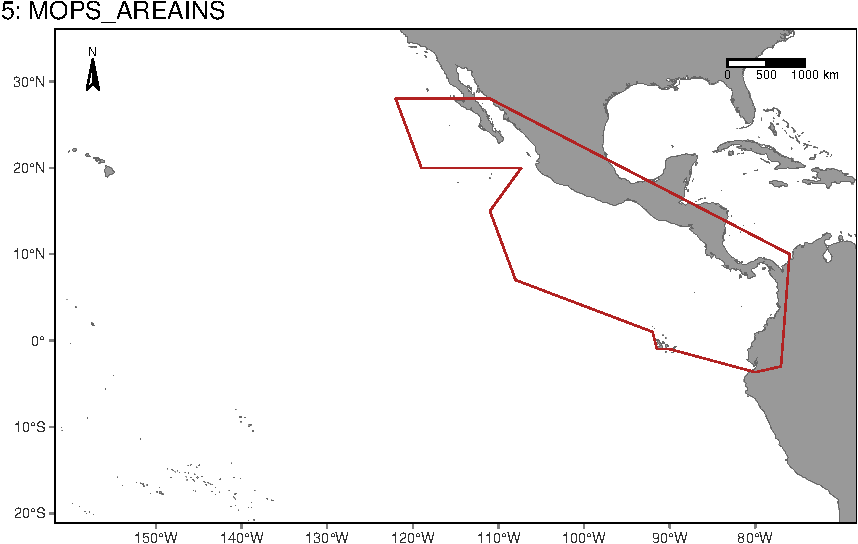
\includegraphics{figures/unnamed-chunk-91-5.pdf} 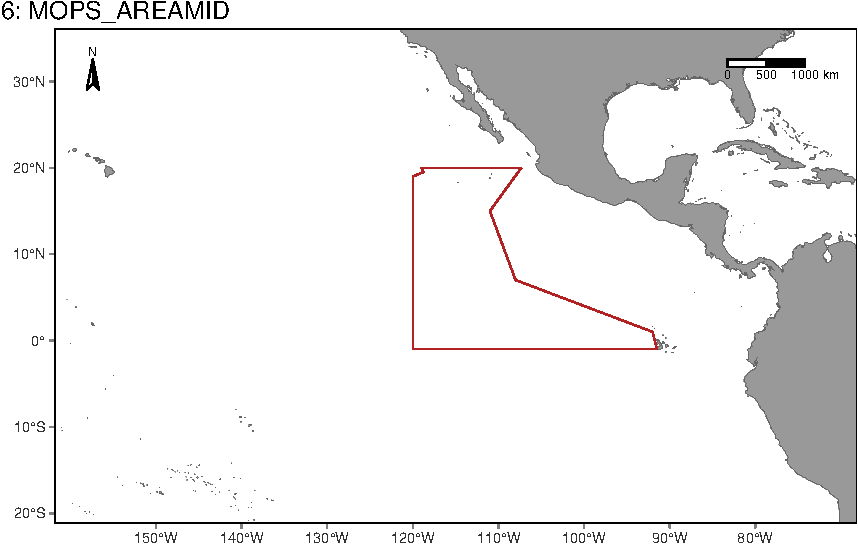
\includegraphics{figures/unnamed-chunk-91-6.pdf} 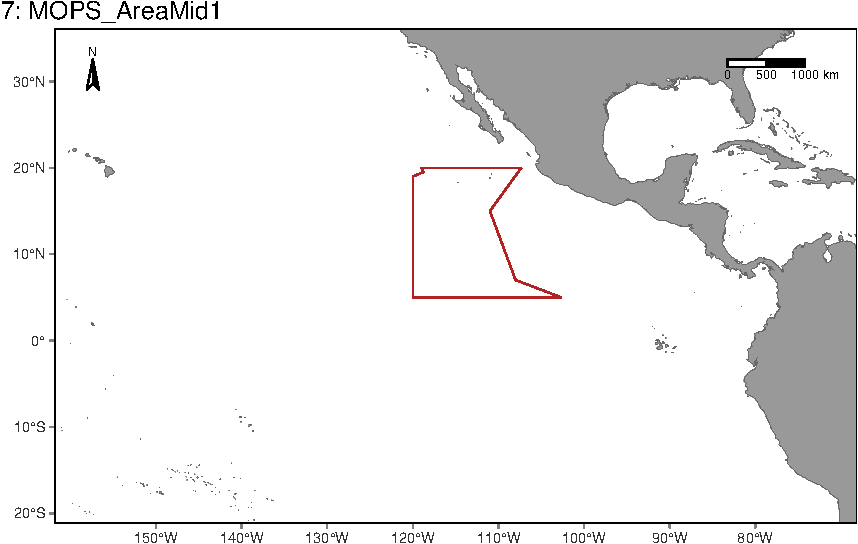
\includegraphics{figures/unnamed-chunk-91-7.pdf} 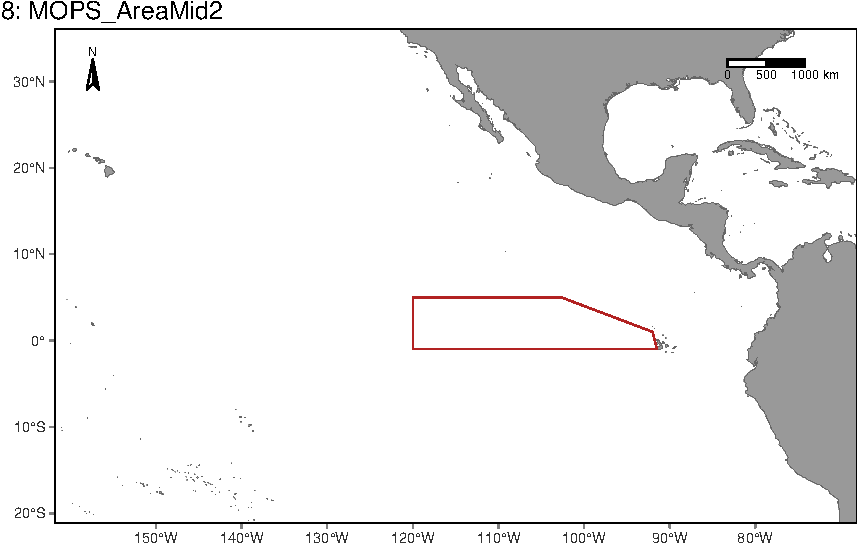
\includegraphics{figures/unnamed-chunk-91-8.pdf} 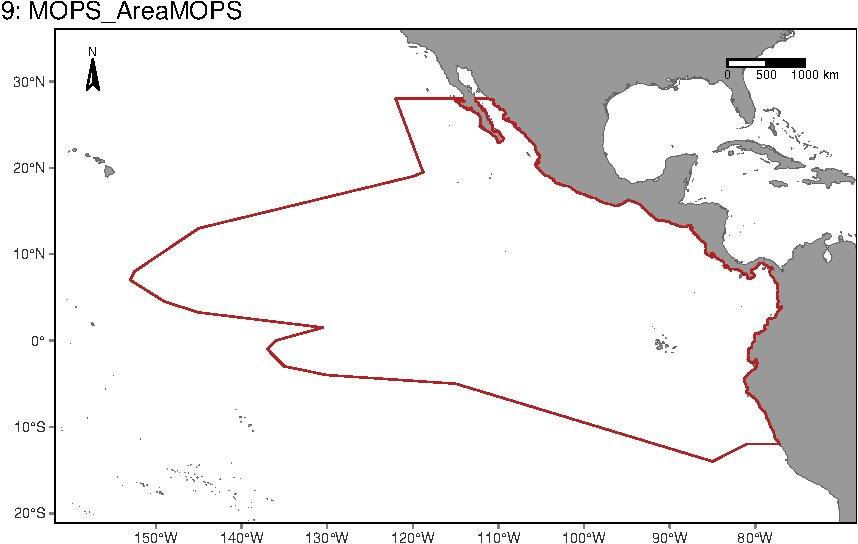
\includegraphics{figures/unnamed-chunk-91-9.pdf} 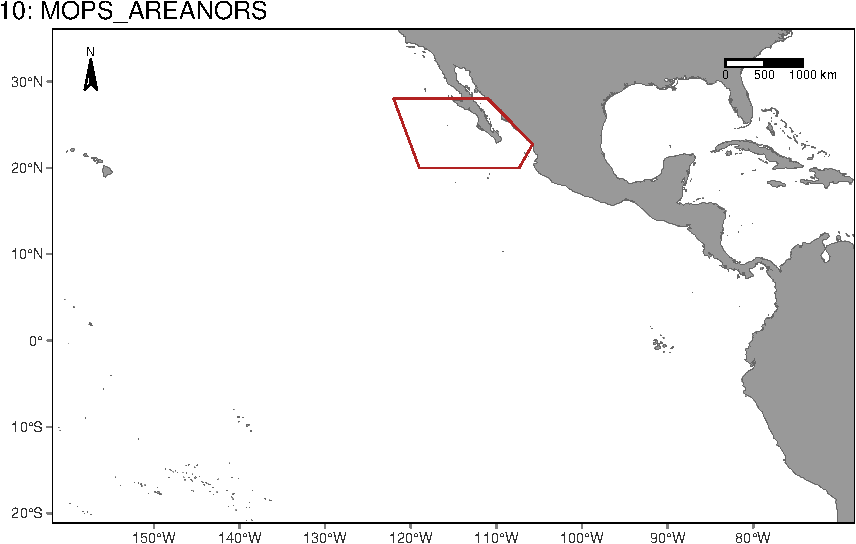
\includegraphics{figures/unnamed-chunk-91-10.pdf} 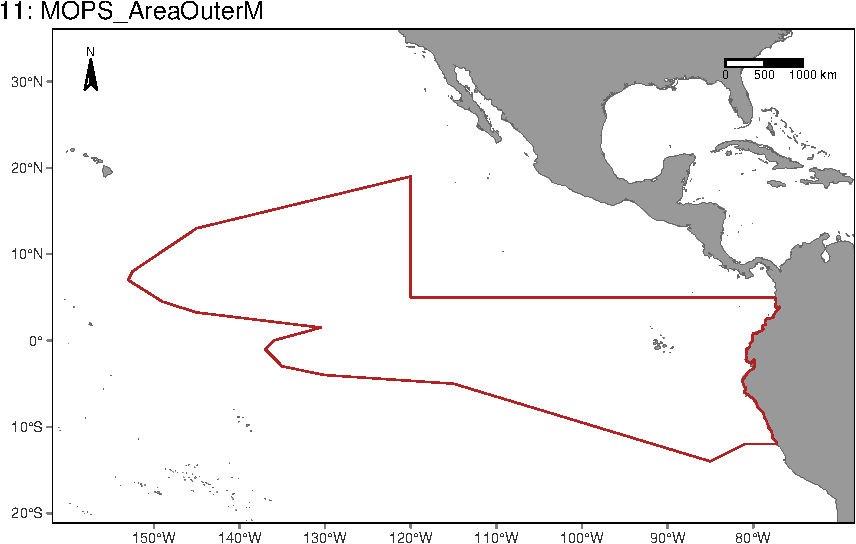
\includegraphics{figures/unnamed-chunk-91-11.pdf} 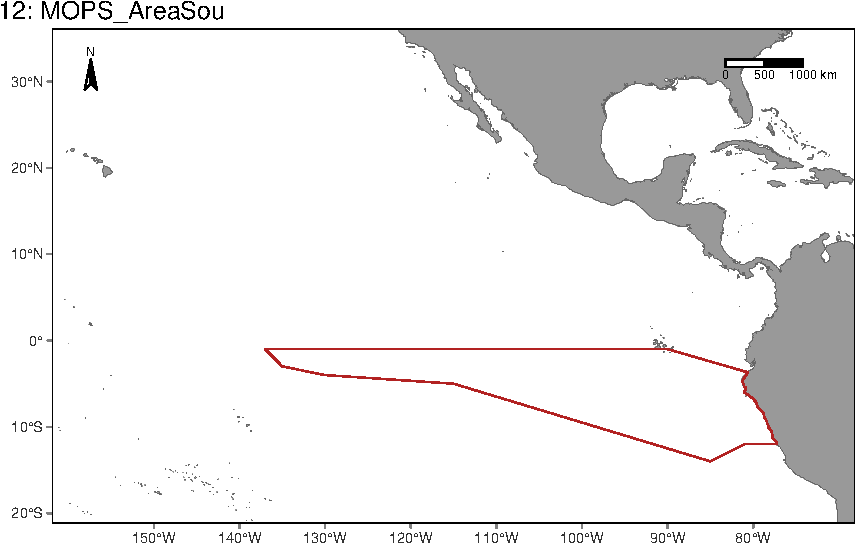
\includegraphics{figures/unnamed-chunk-91-12.pdf} 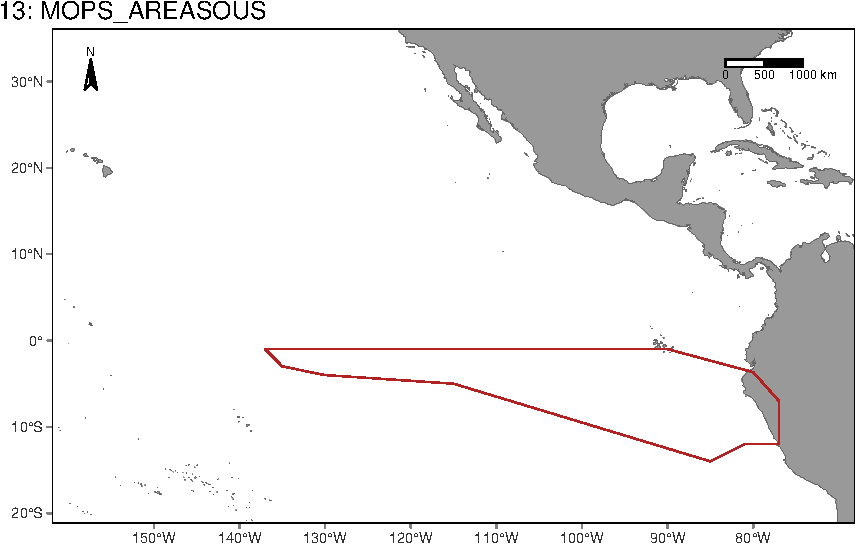
\includegraphics{figures/unnamed-chunk-91-13.pdf} 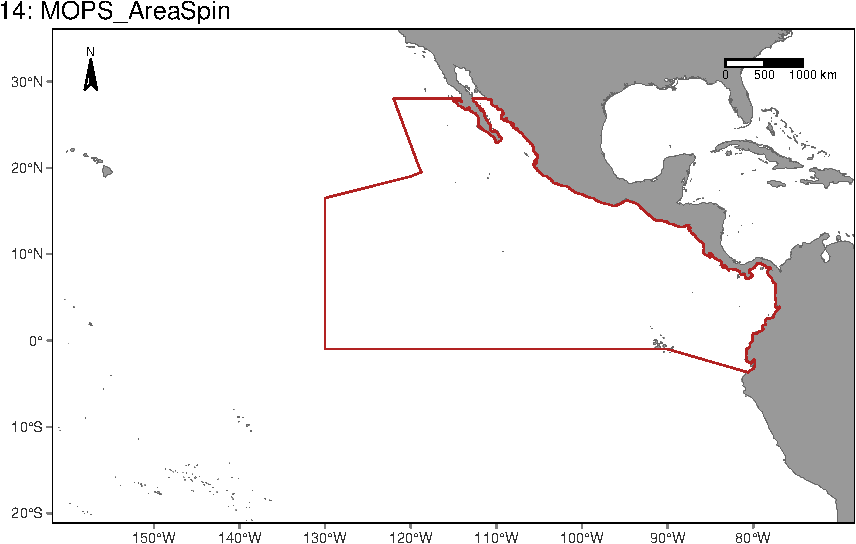
\includegraphics{figures/unnamed-chunk-91-14.pdf} 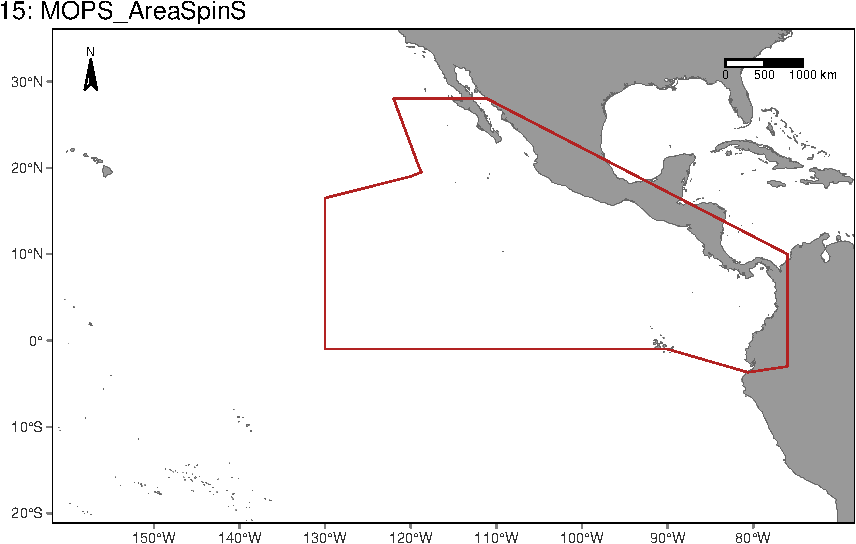
\includegraphics{figures/unnamed-chunk-91-15.pdf} 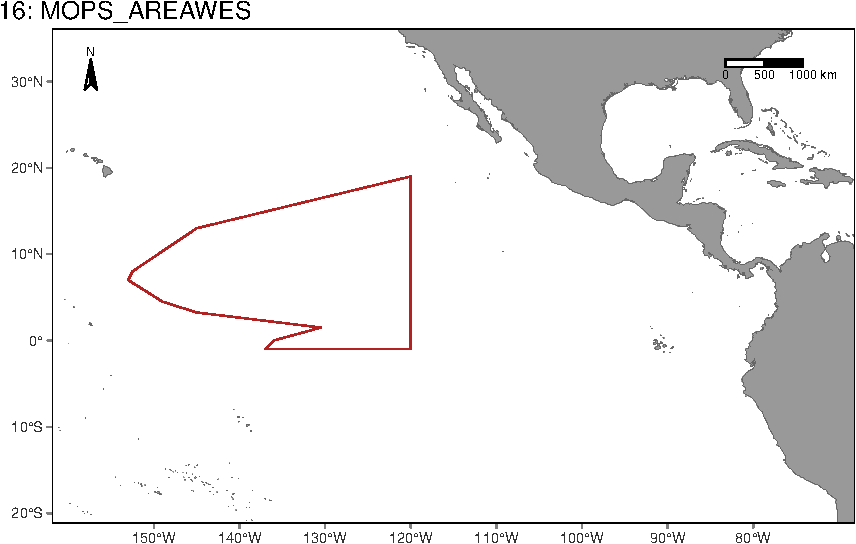
\includegraphics{figures/unnamed-chunk-91-16.pdf} 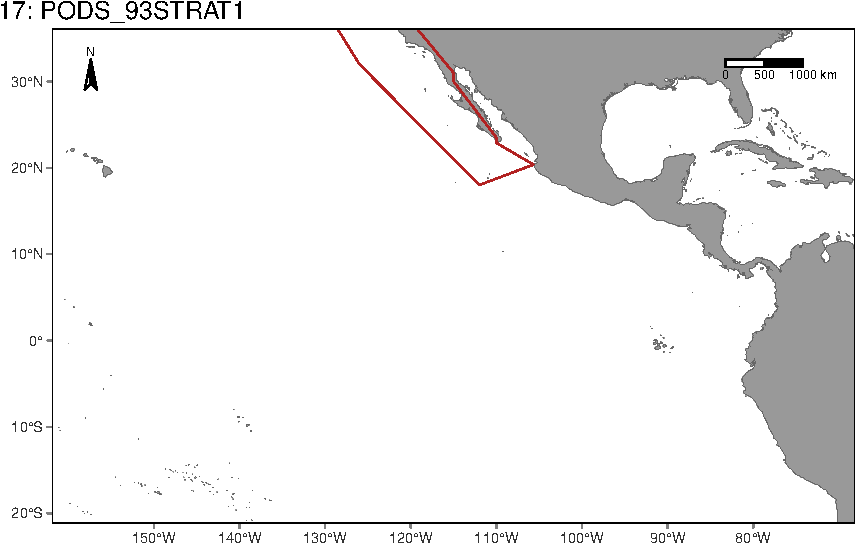
\includegraphics{figures/unnamed-chunk-91-17.pdf} 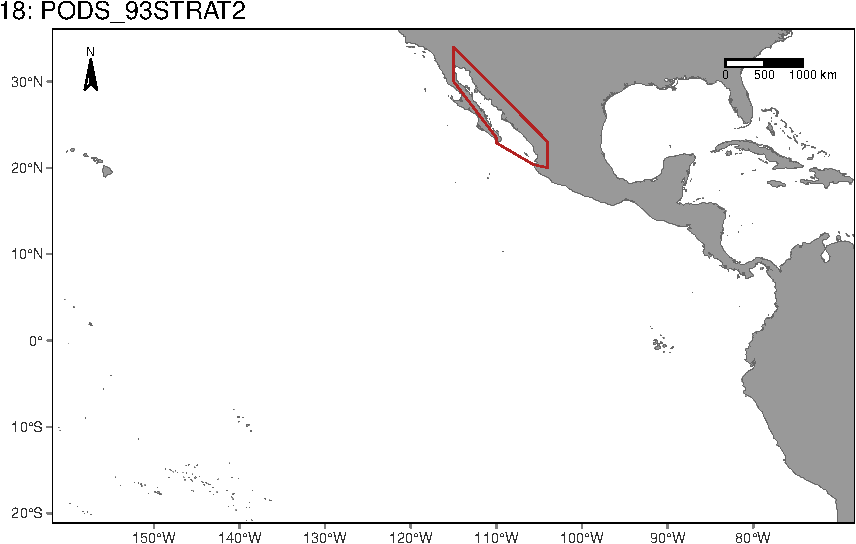
\includegraphics{figures/unnamed-chunk-91-18.pdf} 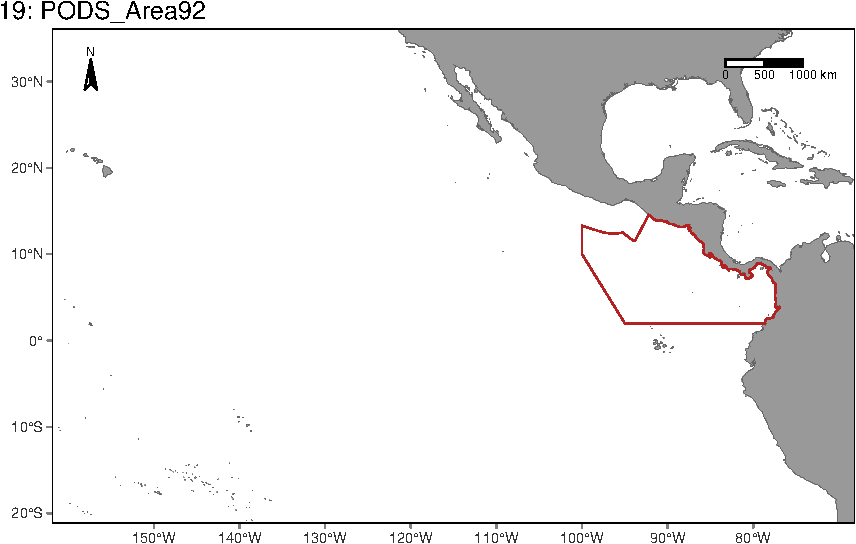
\includegraphics{figures/unnamed-chunk-91-19.pdf} 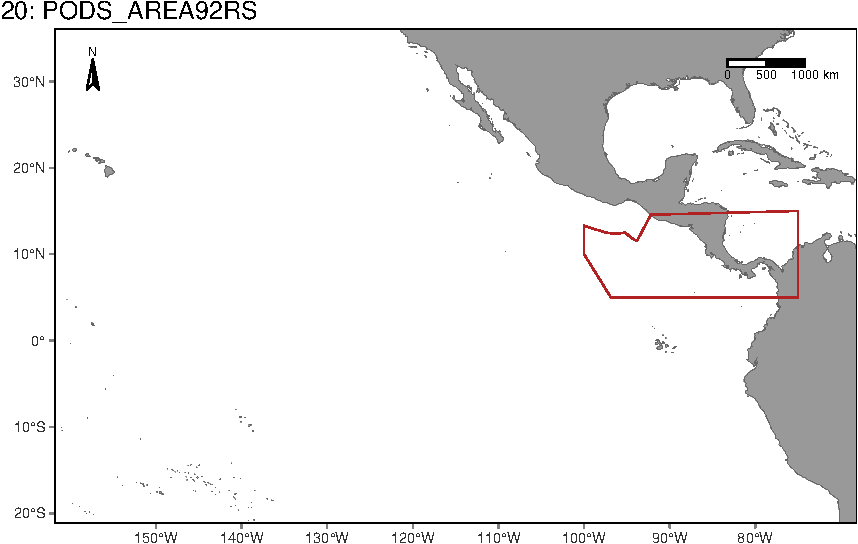
\includegraphics{figures/unnamed-chunk-91-20.pdf} 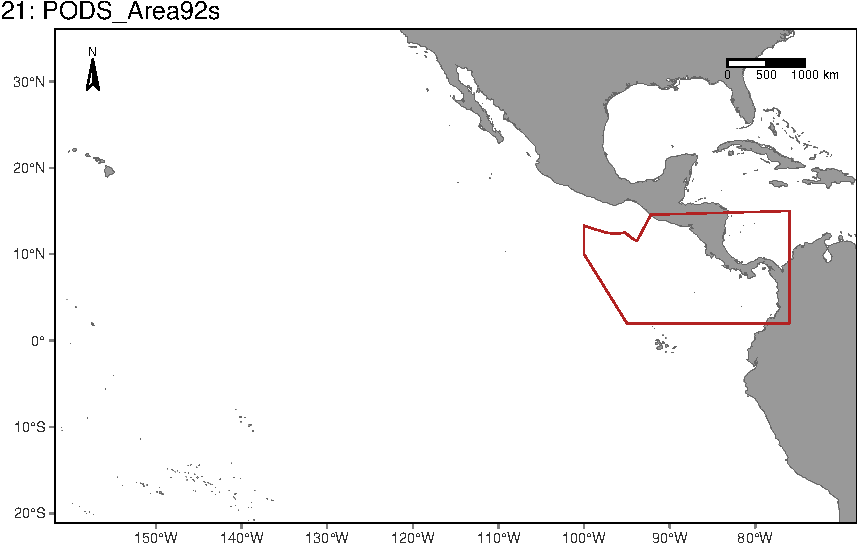
\includegraphics{figures/unnamed-chunk-91-21.pdf} 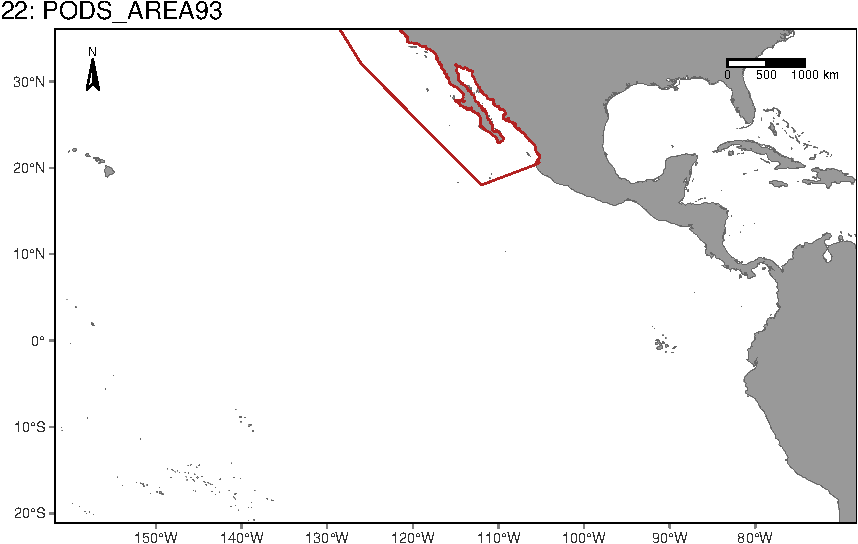
\includegraphics{figures/unnamed-chunk-91-22.pdf} 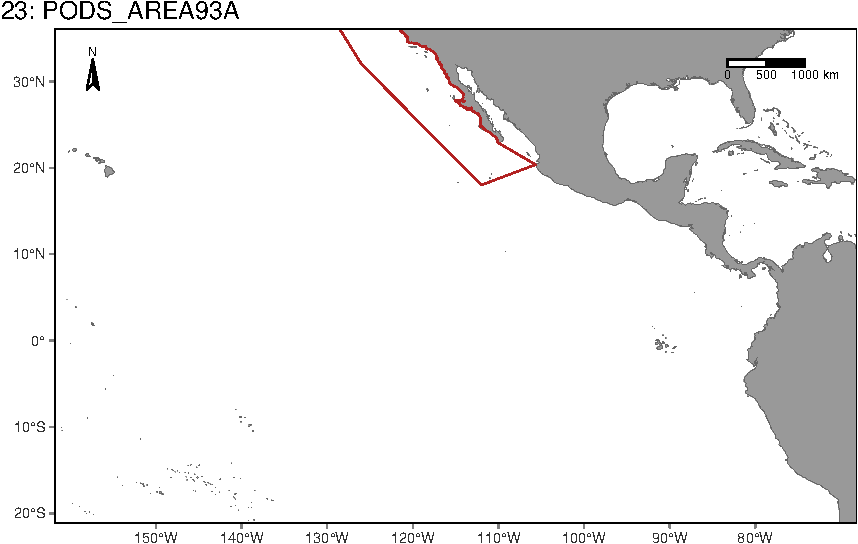
\includegraphics{figures/unnamed-chunk-91-23.pdf} 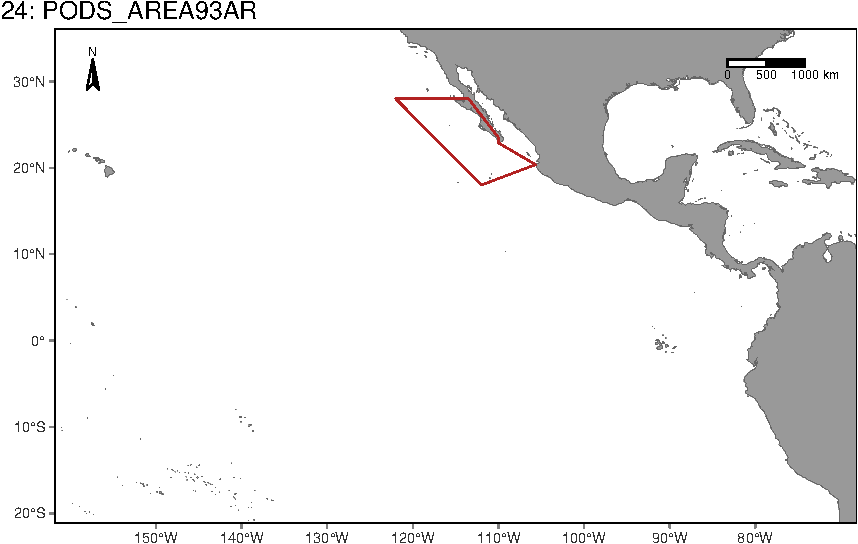
\includegraphics{figures/unnamed-chunk-91-24.pdf} 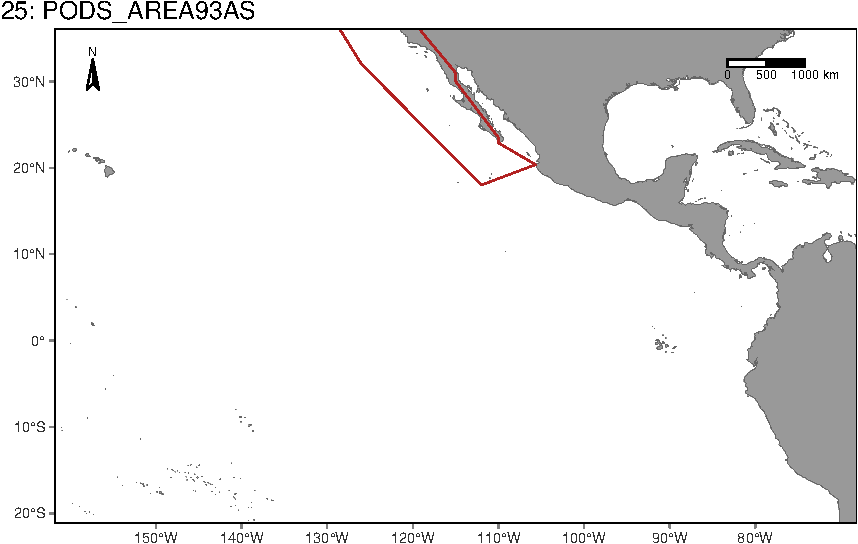
\includegraphics{figures/unnamed-chunk-91-25.pdf} \includegraphics{figures/unnamed-chunk-91-26.pdf} \includegraphics{figures/unnamed-chunk-91-27.pdf} \includegraphics{figures/unnamed-chunk-91-28.pdf} \includegraphics{figures/unnamed-chunk-91-29.pdf} \includegraphics{figures/unnamed-chunk-91-30.pdf} \includegraphics{figures/unnamed-chunk-91-31.pdf} \includegraphics{figures/unnamed-chunk-91-32.pdf} \includegraphics{figures/unnamed-chunk-91-33.pdf} \includegraphics{figures/unnamed-chunk-91-34.pdf} \includegraphics{figures/unnamed-chunk-91-35.pdf} \includegraphics{figures/unnamed-chunk-91-36.pdf} \includegraphics{figures/unnamed-chunk-91-37.pdf} \includegraphics{figures/unnamed-chunk-91-38.pdf} \includegraphics{figures/unnamed-chunk-91-39.pdf} \includegraphics{figures/unnamed-chunk-91-40.pdf} \includegraphics{figures/unnamed-chunk-91-41.pdf} \includegraphics{figures/unnamed-chunk-91-42.pdf} \includegraphics{figures/unnamed-chunk-91-43.pdf} \includegraphics{figures/unnamed-chunk-91-44.pdf} \includegraphics{figures/unnamed-chunk-91-45.pdf} \includegraphics{figures/unnamed-chunk-91-46.pdf} \includegraphics{figures/unnamed-chunk-91-47.pdf} \includegraphics{figures/unnamed-chunk-91-48.pdf} \includegraphics{figures/unnamed-chunk-91-49.pdf} \includegraphics{figures/unnamed-chunk-91-50.pdf} \includegraphics{figures/unnamed-chunk-91-51.pdf} \includegraphics{figures/unnamed-chunk-91-52.pdf} \includegraphics{figures/unnamed-chunk-91-53.pdf} \includegraphics{figures/unnamed-chunk-91-54.pdf} \includegraphics{figures/unnamed-chunk-91-55.pdf} \includegraphics{figures/unnamed-chunk-91-56.pdf} \includegraphics{figures/unnamed-chunk-91-57.pdf} \includegraphics{figures/unnamed-chunk-91-58.pdf} \includegraphics{figures/unnamed-chunk-91-59.pdf} \includegraphics{figures/unnamed-chunk-91-60.pdf} \includegraphics{figures/unnamed-chunk-91-61.pdf} \includegraphics{figures/unnamed-chunk-91-62.pdf} \includegraphics{figures/unnamed-chunk-91-63.pdf} \includegraphics{figures/unnamed-chunk-91-64.pdf} \includegraphics{figures/unnamed-chunk-91-65.pdf} \includegraphics{figures/unnamed-chunk-91-66.pdf} \includegraphics{figures/unnamed-chunk-91-67.pdf} \includegraphics{figures/unnamed-chunk-91-68.pdf} \includegraphics{figures/unnamed-chunk-91-69.pdf} \includegraphics{figures/unnamed-chunk-91-70.pdf}

\hypertarget{segmentizing}{%
\chapter{Segmentizing}\label{segmentizing}}

The package's \texttt{segmentize()} function and its associated settings were designed to give researchers full control over how data are segmented, be it for design-based density analysis (which tend to use long segments of 100 km or more and allow for non-contiguous effort to be included in the same segment) or for habitat modeling (which tend to use short segments of 5 - 10 km and disallow non-contiguous effort to be pooled into the same segment).

\hypertarget{approach}{%
\section*{Approach}\label{approach}}
\addcontentsline{toc}{section}{Approach}

\begin{itemize}
\item
  Segments are built and stored separately for each cohort of species, since each cohort has specific settings for segmentizing.
\item
  Within each cohort, two different sets of segments may be built, in the event that any of the cohort-specific settings for detection function estimation (\texttt{distance\_types}, \texttt{distance\_modes}, and \texttt{distance\_on\_off}) are different from the settings for density estimation (\texttt{density\_types}, \texttt{density\_modes}, and \texttt{density\_on\_off}). When that happens, each cohort will have two lists, one for each analysis: a slot for \texttt{density} segments and their derivated datasets, and a slot for \texttt{distance} segments and derivative data.
\item
  Within each cohort-analysis, the survey is first grouped into ``blocs'' of data that all share the same ``effort scenario'', i.e., all rows share the same Cruise number, study area status (in or out), geographic stratum, and year. Since a survey may leave a stratum then return to it many days hence, it is normal for these blocs to contain non-contiguous data with large spatial gaps. These gaps will be addressed a few steps down.
\item
  The blocs are split further according to survey-wide and cohort-specific settings; for example, if \texttt{segment\_type\_handling} input is \texttt{"separate"}, then data with \texttt{EffType\ =\ "S"} will all belong in its own block, and data with \texttt{EffType\ =\ "N"} will belong in its own bloc, etc.
\item
  The blocs are split a final time according to whether the effort scenario meets inclusion criteria for the analysis. These inclusion criteria are controlled by the cohort-specific settings such as \texttt{density\_types}, \texttt{density\_modes}, and \texttt{density\_in\_off}. Rows of data that meet the inclusion criteria are relegated to their own data bloc, and given a new column, \texttt{use}, with the value \texttt{TRUE}. Data that do \emph{not} meet the criteria are relegated to their own bloc as well (column \texttt{use} is \texttt{FALSE}). This means that, at the end of this process, we will have segments that \emph{will} be used in the density/detection function analysis, and segments that will \emph{not}. (The excluded segments are not deleted or transformed in any other way; they can still be used in summarizing detections, etc.)
\item
  Next, the \texttt{segmentize()} function loops through each of these blocs of effort and parses its data into segments according to the \texttt{segment\_method}. If segmentizing by \texttt{"day"}, this is straightforward: all data occurring on a unique date are assigned to its own segment. Segmentizing by \texttt{"equallength"} is a bit more complicated in terms of coding: segments are built up one line of data at a time; if the \texttt{segment\_target\_km} is reached or the \texttt{segment\_max\_interval} is exceeded, a new segment is begun.
\end{itemize}

At the end of this process, you have lists of data sorted into their segments, each with a unique \texttt{seg\_id}, as well as a summary dataframe that provides the distance (km); time and coordinates for the beginning, middle, and end of the segment; and the weighted averages of sighting conditions and weather data contained in the segment.

\hypertarget{setting-up-this-demo}{%
\subsection*{Setting up this demo}\label{setting-up-this-demo}}
\addcontentsline{toc}{subsection}{Setting up this demo}

The demonstration of \texttt{segmentize()} on in \protect\hyperlink{processing}{Processing chapter} relies on the \texttt{settings} list that is attached as a slot in the \texttt{cruz} object. But you can override those settings with direct function inputs in \texttt{segmentize()}, which gives us a chance to explore segmentization options.

First we load the demo data and carry out initial processing:

\begin{Shaded}
\begin{Highlighting}[]
\KeywordTok{data}\NormalTok{(settings)}
\NormalTok{das_file <-}\StringTok{ 'data/surveys/HICEASwinter2020.das'}
\NormalTok{das <-}\StringTok{ }\KeywordTok{load_das}\NormalTok{(das_file, }
                \DataTypeTok{perform_checks =} \OtherTok{FALSE}\NormalTok{,}
                \DataTypeTok{print_glimpse =} \OtherTok{FALSE}\NormalTok{)}
\NormalTok{cruz <-}\StringTok{ }\KeywordTok{process_strata}\NormalTok{(das,}
\NormalTok{                       settings,}
                       \DataTypeTok{verbose=}\OtherTok{FALSE}\NormalTok{)}
\NormalTok{cruz <-}\StringTok{ }\KeywordTok{format_das}\NormalTok{(cruz)}
\end{Highlighting}
\end{Shaded}

And this is the histogram function we will be using to display the results of each run of \texttt{segmentize()}:

\begin{Shaded}
\begin{Highlighting}[]
\NormalTok{segment_histogram <-}\StringTok{ }\ControlFlowTok{function}\NormalTok{(cohort_effort, }\DataTypeTok{by_day=}\OtherTok{FALSE}\NormalTok{)\{}
\NormalTok{  segs <-}\StringTok{ }\NormalTok{cohort_effort}\OperatorTok{$}\NormalTok{segments}
\NormalTok{  segmax <-}\StringTok{ }\KeywordTok{max}\NormalTok{(segs}\OperatorTok{$}\NormalTok{dist,}\DataTypeTok{na.rm=}\OtherTok{TRUE}\NormalTok{)}\OperatorTok{*}\FloatTok{1.1}
  
  \ControlFlowTok{if}\NormalTok{(by_day)\{}
\NormalTok{    main_use <-}\StringTok{ }\KeywordTok{paste0}\NormalTok{(}\StringTok{'Segments (use) |  by day'}\NormalTok{)}
\NormalTok{    main_exclude <-}\StringTok{ }\KeywordTok{paste0}\NormalTok{(}\StringTok{'Segments (exclude) |  by day'}\NormalTok{)}
\NormalTok{  \}}\ControlFlowTok{else}\NormalTok{\{}
\NormalTok{    main_use <-}\StringTok{ }\KeywordTok{paste0}\NormalTok{(}\StringTok{'Segments (use) |  target: '}\NormalTok{,settings}\OperatorTok{$}\NormalTok{survey}\OperatorTok{$}\NormalTok{segment_target_km,}\StringTok{' km'}\NormalTok{)}
\NormalTok{    main_exclude <-}\StringTok{ }\KeywordTok{paste0}\NormalTok{(}\StringTok{'Segments (exclude) |  target: '}\NormalTok{,settings}\OperatorTok{$}\NormalTok{survey}\OperatorTok{$}\NormalTok{segment_target_km,}\StringTok{' km'}\NormalTok{)}
\NormalTok{  \}}
  \KeywordTok{par}\NormalTok{(}\DataTypeTok{mfrow=}\KeywordTok{c}\NormalTok{(}\DecValTok{1}\NormalTok{,}\DecValTok{2}\NormalTok{))}
  \KeywordTok{par}\NormalTok{(}\DataTypeTok{mar=}\KeywordTok{c}\NormalTok{(}\FloatTok{4.2}\NormalTok{,}\FloatTok{4.2}\NormalTok{,}\FloatTok{2.5}\NormalTok{,.}\DecValTok{5}\NormalTok{))}
  \KeywordTok{hist}\NormalTok{(segs}\OperatorTok{$}\NormalTok{dist[segs}\OperatorTok{$}\NormalTok{use],}
       \DataTypeTok{breaks =} \KeywordTok{seq}\NormalTok{(}\DecValTok{0}\NormalTok{,segmax,}\DataTypeTok{by=}\NormalTok{segmax}\OperatorTok{/}\DecValTok{40}\NormalTok{),}
       \DataTypeTok{xlab=}\StringTok{'Segment lengths (km)'}\NormalTok{,}
       \DataTypeTok{main=}\NormalTok{main_use,}
       \DataTypeTok{cex.main =} \FloatTok{.8}\NormalTok{, }\DataTypeTok{cex.axis =} \FloatTok{.8}\NormalTok{, }\DataTypeTok{cex.lab =} \FloatTok{.8}\NormalTok{)}

  \KeywordTok{hist}\NormalTok{(segs}\OperatorTok{$}\NormalTok{dist[}\OperatorTok{!}\NormalTok{segs}\OperatorTok{$}\NormalTok{use],}
       \DataTypeTok{breaks =} \KeywordTok{seq}\NormalTok{(}\DecValTok{0}\NormalTok{,segmax,}\DataTypeTok{by=}\NormalTok{segmax}\OperatorTok{/}\DecValTok{40}\NormalTok{),}
       \DataTypeTok{xlab=}\StringTok{'Segment lengths (km)'}\NormalTok{,}
       \DataTypeTok{main=}\NormalTok{main_exclude,}
       \DataTypeTok{cex.main =} \FloatTok{.8}\NormalTok{, }\DataTypeTok{cex.axis =} \FloatTok{.8}\NormalTok{, }\DataTypeTok{cex.lab =} \FloatTok{.8}\NormalTok{)}
  \KeywordTok{par}\NormalTok{(}\DataTypeTok{mfrow=}\KeywordTok{c}\NormalTok{(}\DecValTok{1}\NormalTok{,}\DecValTok{1}\NormalTok{))}
\NormalTok{\}}
\end{Highlighting}
\end{Shaded}

\hypertarget{defaults-2}{%
\section*{Defaults}\label{defaults-2}}
\addcontentsline{toc}{section}{Defaults}

Here is the \texttt{segmentize()} function parameterized with the ``factory default'' settings from \texttt{load\_settings()}.

\begin{Shaded}
\begin{Highlighting}[]
\NormalTok{cruz_demo <-}\StringTok{ }\KeywordTok{segmentize}\NormalTok{(cruz,}
                        \DataTypeTok{segment_method =} \StringTok{'equallength'}\NormalTok{,}
                        \DataTypeTok{segment_target_km =} \DecValTok{30}\NormalTok{,}
                        \DataTypeTok{segment_max_interval =} \DecValTok{48}\NormalTok{,}
                        \DataTypeTok{segment_type_handling =} \StringTok{'separate'}\NormalTok{,}
                        \DataTypeTok{segment_remainder_handling =} \KeywordTok{c}\NormalTok{(}\StringTok{'append'}\NormalTok{,}\StringTok{'segment'}\NormalTok{),}
                        \DataTypeTok{density_types =} \KeywordTok{c}\NormalTok{(}\StringTok{'S'}\NormalTok{,}\StringTok{'F'}\NormalTok{),}
                        \DataTypeTok{density_modes =} \KeywordTok{c}\NormalTok{(}\StringTok{'P'}\NormalTok{,}\StringTok{'C'}\NormalTok{),}
                        \DataTypeTok{density_on_off =} \KeywordTok{c}\NormalTok{(}\OtherTok{TRUE}\NormalTok{),}
                        \DataTypeTok{distance_types =} \OtherTok{NULL}\NormalTok{,}
                        \DataTypeTok{distance_modes =} \OtherTok{NULL}\NormalTok{,}
                        \DataTypeTok{distance_on_off =} \OtherTok{NULL}\NormalTok{,}
                        \DataTypeTok{random_seed =} \OtherTok{NULL}\NormalTok{)}

\CommentTok{# Number of segments}
\NormalTok{cruz_demo}\OperatorTok{$}\NormalTok{cohorts}\OperatorTok{$}\NormalTok{default}\OperatorTok{$}\NormalTok{density}\OperatorTok{$}\NormalTok{segments }\OperatorTok\StringTok{ }\NormalTok{nrow}
\NormalTok{[}\DecValTok{1}\NormalTok{] }\DecValTok{268}

\CommentTok{# Plot}
\KeywordTok{segment_histogram}\NormalTok{(cruz_demo}\OperatorTok{$}\NormalTok{cohorts}\OperatorTok{$}\NormalTok{default}\OperatorTok{$}\NormalTok{density)}
\end{Highlighting}
\end{Shaded}

\includegraphics{figures/unnamed-chunk-95-1.pdf}

\hypertarget{day-vs-equal-length}{%
\section*{Day vs Equal Length}\label{day-vs-equal-length}}
\addcontentsline{toc}{section}{Day vs Equal Length}

\hypertarget{by-day}{%
\subsection*{By day}\label{by-day}}
\addcontentsline{toc}{subsection}{By day}

\begin{Shaded}
\begin{Highlighting}[]
\NormalTok{cruz_demo <-}\StringTok{ }\KeywordTok{segmentize}\NormalTok{(cruz,}
                        \DataTypeTok{segment_method =} \StringTok{'day'}\NormalTok{,}
                        \DataTypeTok{segment_target_km =} \DecValTok{30}\NormalTok{,}
                        \DataTypeTok{segment_max_interval =} \DecValTok{48}\NormalTok{,}
                        \DataTypeTok{segment_type_handling =} \StringTok{'separate'}\NormalTok{,}
                        \DataTypeTok{segment_remainder_handling =} \KeywordTok{c}\NormalTok{(}\StringTok{'append'}\NormalTok{,}\StringTok{'segment'}\NormalTok{),}
                        \DataTypeTok{density_types =} \KeywordTok{c}\NormalTok{(}\StringTok{'S'}\NormalTok{,}\StringTok{'F'}\NormalTok{),}
                        \DataTypeTok{density_modes =} \KeywordTok{c}\NormalTok{(}\StringTok{'P'}\NormalTok{,}\StringTok{'C'}\NormalTok{),}
                        \DataTypeTok{density_on_off =} \KeywordTok{c}\NormalTok{(}\OtherTok{TRUE}\NormalTok{),}
                        \DataTypeTok{distance_types =} \OtherTok{NULL}\NormalTok{,}
                        \DataTypeTok{distance_modes =} \OtherTok{NULL}\NormalTok{,}
                        \DataTypeTok{distance_on_off =} \OtherTok{NULL}\NormalTok{,}
                        \DataTypeTok{random_seed =} \OtherTok{NULL}\NormalTok{)}

\CommentTok{# Number of segments}
\NormalTok{cruz_demo}\OperatorTok{$}\NormalTok{cohorts}\OperatorTok{$}\NormalTok{default}\OperatorTok{$}\NormalTok{density}\OperatorTok{$}\NormalTok{segments }\OperatorTok\StringTok{ }\NormalTok{nrow}
\NormalTok{[}\DecValTok{1}\NormalTok{] }\DecValTok{96}

\CommentTok{# Plot}
\KeywordTok{segment_histogram}\NormalTok{(cruz_demo}\OperatorTok{$}\NormalTok{cohorts}\OperatorTok{$}\NormalTok{default}\OperatorTok{$}\NormalTok{density, }\DataTypeTok{by_day =} \OtherTok{TRUE}\NormalTok{)}
\end{Highlighting}
\end{Shaded}

\includegraphics{figures/unnamed-chunk-97-1.pdf}

\hypertarget{by-target-length-of-150-km}{%
\subsection*{By target length of 150 km}\label{by-target-length-of-150-km}}
\addcontentsline{toc}{subsection}{By target length of 150 km}

\begin{Shaded}
\begin{Highlighting}[]
\NormalTok{cruz_demo <-}\StringTok{ }\KeywordTok{segmentize}\NormalTok{(cruz,}
                        \DataTypeTok{segment_method =} \StringTok{'equallength'}\NormalTok{,}
                        \DataTypeTok{segment_target_km =} \DecValTok{150}\NormalTok{,}
                        \DataTypeTok{segment_max_interval =} \DecValTok{48}\NormalTok{,}
                        \DataTypeTok{segment_type_handling =} \StringTok{'separate'}\NormalTok{,}
                        \DataTypeTok{segment_remainder_handling =} \KeywordTok{c}\NormalTok{(}\StringTok{'append'}\NormalTok{,}\StringTok{'segment'}\NormalTok{),}
                        \DataTypeTok{density_types =} \KeywordTok{c}\NormalTok{(}\StringTok{'S'}\NormalTok{,}\StringTok{'F'}\NormalTok{),}
                        \DataTypeTok{density_modes =} \KeywordTok{c}\NormalTok{(}\StringTok{'P'}\NormalTok{,}\StringTok{'C'}\NormalTok{),}
                        \DataTypeTok{density_on_off =} \KeywordTok{c}\NormalTok{(}\OtherTok{TRUE}\NormalTok{),}
                        \DataTypeTok{distance_types =} \OtherTok{NULL}\NormalTok{,}
                        \DataTypeTok{distance_modes =} \OtherTok{NULL}\NormalTok{,}
                        \DataTypeTok{distance_on_off =} \OtherTok{NULL}\NormalTok{,}
                        \DataTypeTok{random_seed =} \OtherTok{NULL}\NormalTok{)}

\CommentTok{# Number of segments}
\NormalTok{cruz_demo}\OperatorTok{$}\NormalTok{cohorts}\OperatorTok{$}\NormalTok{default}\OperatorTok{$}\NormalTok{density}\OperatorTok{$}\NormalTok{segments }\OperatorTok\StringTok{ }\NormalTok{nrow}
\NormalTok{[}\DecValTok{1}\NormalTok{] }\DecValTok{60}

\CommentTok{# Plot}
\KeywordTok{segment_histogram}\NormalTok{(cruz_demo}\OperatorTok{$}\NormalTok{cohorts}\OperatorTok{$}\NormalTok{default}\OperatorTok{$}\NormalTok{density, }\DataTypeTok{by_day =} \OtherTok{TRUE}\NormalTok{)}
\end{Highlighting}
\end{Shaded}

\includegraphics{figures/unnamed-chunk-98-1.pdf}

\hypertarget{contiguous-vs.-non-contiguous-effort}{%
\section*{Contiguous vs.~non-contiguous effort}\label{contiguous-vs.-non-contiguous-effort}}
\addcontentsline{toc}{section}{Contiguous vs.~non-contiguous effort}

The example above allows for non-contiguous effort; a segment is allowed to contain effort separated by gaps as large as 24 hours (\texttt{settings\$max\_interval}). To coerce segments to represent only contiguous effort, make that setting very small:

\begin{Shaded}
\begin{Highlighting}[]
\NormalTok{cruz_demo <-}\StringTok{ }\KeywordTok{segmentize}\NormalTok{(cruz,}
                        \DataTypeTok{segment_method =} \StringTok{'equallength'}\NormalTok{,}
                        \DataTypeTok{segment_target_km =} \DecValTok{30}\NormalTok{,}
                        \DataTypeTok{segment_max_interval =} \FloatTok{.1}\NormalTok{,}
                        \DataTypeTok{segment_type_handling =} \StringTok{'separate'}\NormalTok{,}
                        \DataTypeTok{segment_remainder_handling =} \KeywordTok{c}\NormalTok{(}\StringTok{'append'}\NormalTok{,}\StringTok{'segment'}\NormalTok{),}
                        \DataTypeTok{density_types =} \KeywordTok{c}\NormalTok{(}\StringTok{'S'}\NormalTok{,}\StringTok{'F'}\NormalTok{),}
                        \DataTypeTok{density_modes =} \KeywordTok{c}\NormalTok{(}\StringTok{'P'}\NormalTok{,}\StringTok{'C'}\NormalTok{),}
                        \DataTypeTok{density_on_off =} \KeywordTok{c}\NormalTok{(}\OtherTok{TRUE}\NormalTok{),}
                        \DataTypeTok{distance_types =} \OtherTok{NULL}\NormalTok{,}
                        \DataTypeTok{distance_modes =} \OtherTok{NULL}\NormalTok{,}
                        \DataTypeTok{distance_on_off =} \OtherTok{NULL}\NormalTok{,}
                        \DataTypeTok{random_seed =} \OtherTok{NULL}\NormalTok{)}

\CommentTok{# Number of segments}
\NormalTok{cruz_demo}\OperatorTok{$}\NormalTok{cohorts}\OperatorTok{$}\NormalTok{default}\OperatorTok{$}\NormalTok{density}\OperatorTok{$}\NormalTok{segments }\OperatorTok\StringTok{ }\NormalTok{nrow}
\NormalTok{[}\DecValTok{1}\NormalTok{] }\DecValTok{504}

\CommentTok{# Plot}
\KeywordTok{segment_histogram}\NormalTok{(cruz_demo}\OperatorTok{$}\NormalTok{cohorts}\OperatorTok{$}\NormalTok{default}\OperatorTok{$}\NormalTok{density, }\DataTypeTok{by_day =} \OtherTok{TRUE}\NormalTok{)}
\end{Highlighting}
\end{Shaded}

\includegraphics{figures/unnamed-chunk-99-1.pdf}

You can see that many contiguous periods of effort were much shorter than the target length of 30 km. This is why allowing for non-contiguous effort can be advantageous for target segment lengths larger than 5 - 10 km.

\hypertarget{segment-remainder-handling}{%
\section*{Segment remainder handling}\label{segment-remainder-handling}}
\addcontentsline{toc}{section}{Segment remainder handling}

The default setting for \texttt{segment\_remainder\_handling}, \texttt{c(\textquotesingle{}append\textquotesingle{},\textquotesingle{}segment\textquotesingle{})}, means that remainders less than half the target length will be randomly appended to another segment, while remainders more than half will be treated as their own segment (and will be placed randomly along the trackline).

If you don't want that level of complexity, you can simply assign a single setting: \texttt{\textquotesingle{}append\textquotesingle{}} will append the remainder in all cases, regardless of remainder length relative to the target length. The same idea goes for \texttt{\textquotesingle{}segment\textquotesingle{}}.

The other possible setting is \texttt{\textquotesingle{}disperse\textquotesingle{}}, which disperses the remainder evenly across all segments. To demonstrate, let's use a target length of 100 km.

\begin{Shaded}
\begin{Highlighting}[]
\NormalTok{cruz_demo <-}\StringTok{ }\KeywordTok{segmentize}\NormalTok{(cruz,}
                        \DataTypeTok{segment_method =} \StringTok{'equallength'}\NormalTok{,}
                        \DataTypeTok{segment_target_km =} \DecValTok{100}\NormalTok{,}
                        \DataTypeTok{segment_max_interval =} \DecValTok{48}\NormalTok{,}
                        \DataTypeTok{segment_type_handling =} \StringTok{'separate'}\NormalTok{,}
                        \DataTypeTok{segment_remainder_handling =} \KeywordTok{c}\NormalTok{(}\StringTok{'disperse'}\NormalTok{),}
                        \DataTypeTok{density_types =} \KeywordTok{c}\NormalTok{(}\StringTok{'S'}\NormalTok{,}\StringTok{'F'}\NormalTok{),}
                        \DataTypeTok{density_modes =} \KeywordTok{c}\NormalTok{(}\StringTok{'P'}\NormalTok{,}\StringTok{'C'}\NormalTok{),}
                        \DataTypeTok{density_on_off =} \KeywordTok{c}\NormalTok{(}\OtherTok{TRUE}\NormalTok{),}
                        \DataTypeTok{distance_types =} \OtherTok{NULL}\NormalTok{,}
                        \DataTypeTok{distance_modes =} \OtherTok{NULL}\NormalTok{,}
                        \DataTypeTok{distance_on_off =} \OtherTok{NULL}\NormalTok{,}
                        \DataTypeTok{random_seed =} \OtherTok{NULL}\NormalTok{)}

\CommentTok{# Number of segments}
\NormalTok{cruz_demo}\OperatorTok{$}\NormalTok{cohorts}\OperatorTok{$}\NormalTok{default}\OperatorTok{$}\NormalTok{density}\OperatorTok{$}\NormalTok{segments }\OperatorTok\StringTok{ }\NormalTok{nrow}
\NormalTok{[}\DecValTok{1}\NormalTok{] }\DecValTok{76}

\CommentTok{# Plot}
\KeywordTok{segment_histogram}\NormalTok{(cruz_demo}\OperatorTok{$}\NormalTok{cohorts}\OperatorTok{$}\NormalTok{default}\OperatorTok{$}\NormalTok{density, }\DataTypeTok{by_day =} \OtherTok{TRUE}\NormalTok{)}
\end{Highlighting}
\end{Shaded}

\includegraphics{figures/unnamed-chunk-100-1.pdf}

Note that most segments are longer than the target length, due to the impact of dispersing the remainder. If you wanted, you could combat this by making the target length slightly smaller:

\begin{Shaded}
\begin{Highlighting}[]
\NormalTok{cruz_demo <-}\StringTok{ }\KeywordTok{segmentize}\NormalTok{(cruz,}
                        \DataTypeTok{segment_method =} \StringTok{'equallength'}\NormalTok{,}
                        \DataTypeTok{segment_target_km =} \DecValTok{90}\NormalTok{,}
                        \DataTypeTok{segment_max_interval =} \DecValTok{48}\NormalTok{,}
                        \DataTypeTok{segment_type_handling =} \StringTok{'separate'}\NormalTok{,}
                        \DataTypeTok{segment_remainder_handling =} \KeywordTok{c}\NormalTok{(}\StringTok{'disperse'}\NormalTok{),}
                        \DataTypeTok{density_types =} \KeywordTok{c}\NormalTok{(}\StringTok{'S'}\NormalTok{,}\StringTok{'F'}\NormalTok{),}
                        \DataTypeTok{density_modes =} \KeywordTok{c}\NormalTok{(}\StringTok{'P'}\NormalTok{,}\StringTok{'C'}\NormalTok{),}
                        \DataTypeTok{density_on_off =} \KeywordTok{c}\NormalTok{(}\OtherTok{TRUE}\NormalTok{),}
                        \DataTypeTok{distance_types =} \OtherTok{NULL}\NormalTok{,}
                        \DataTypeTok{distance_modes =} \OtherTok{NULL}\NormalTok{,}
                        \DataTypeTok{distance_on_off =} \OtherTok{NULL}\NormalTok{,}
                        \DataTypeTok{random_seed =} \OtherTok{NULL}\NormalTok{)}

\CommentTok{# Number of segments}
\NormalTok{cruz_demo}\OperatorTok{$}\NormalTok{cohorts}\OperatorTok{$}\NormalTok{default}\OperatorTok{$}\NormalTok{density}\OperatorTok{$}\NormalTok{segments }\OperatorTok\StringTok{ }\NormalTok{nrow}
\NormalTok{[}\DecValTok{1}\NormalTok{] }\DecValTok{86}

\CommentTok{# Plot}
\KeywordTok{segment_histogram}\NormalTok{(cruz_demo}\OperatorTok{$}\NormalTok{cohorts}\OperatorTok{$}\NormalTok{default}\OperatorTok{$}\NormalTok{density, }\DataTypeTok{by_day =} \OtherTok{TRUE}\NormalTok{)}
\end{Highlighting}
\end{Shaded}

\includegraphics{figures/unnamed-chunk-101-1.pdf}

But in general, the \texttt{disperse} option may be more appropriate for shorter segment lengths.

\hypertarget{typical-settings}{%
\section*{Typical settings}\label{typical-settings}}
\addcontentsline{toc}{section}{Typical settings}

\hypertarget{design-based-line-transect-analysis}{%
\subsection*{Design-based line transect analysis}\label{design-based-line-transect-analysis}}
\addcontentsline{toc}{subsection}{Design-based line transect analysis}

To replicate methods used in density estimation analyses, use large segment lengths (100 km or more) or simply segmentize by day, with \texttt{S} and \texttt{F} effort types kept separate. (See the examples above.) Remember that long segment lengths won't work well unless you allow for non-contiguous effort.

\hypertarget{habitat-modeling}{%
\subsection*{Habitat modeling}\label{habitat-modeling}}
\addcontentsline{toc}{subsection}{Habitat modeling}

To replicate the methods used in typical habitat modeling studies, use smaller segment lengths of contiguous effort. In these studies it may be acceptable to pool various effort types into the same segments.

\begin{Shaded}
\begin{Highlighting}[]
\NormalTok{cruz_demo <-}\StringTok{ }\KeywordTok{segmentize}\NormalTok{(cruz,}
                        \DataTypeTok{segment_method =} \StringTok{'equallength'}\NormalTok{,}
                        \DataTypeTok{segment_target_km =} \DecValTok{5}\NormalTok{,}
                        \DataTypeTok{segment_max_interval =} \FloatTok{.1}\NormalTok{,}
                        \DataTypeTok{segment_type_handling =} \StringTok{'pool'}\NormalTok{,}
                        \DataTypeTok{segment_remainder_handling =} \KeywordTok{c}\NormalTok{(}\StringTok{'append'}\NormalTok{,}\StringTok{'segment'}\NormalTok{),}
                        \DataTypeTok{density_types =} \KeywordTok{c}\NormalTok{(}\StringTok{'S'}\NormalTok{,}\StringTok{'F'}\NormalTok{),}
                        \DataTypeTok{density_modes =} \KeywordTok{c}\NormalTok{(}\StringTok{'P'}\NormalTok{,}\StringTok{'C'}\NormalTok{),}
                        \DataTypeTok{density_on_off =} \KeywordTok{c}\NormalTok{(}\OtherTok{TRUE}\NormalTok{),}
                        \DataTypeTok{distance_types =} \OtherTok{NULL}\NormalTok{,}
                        \DataTypeTok{distance_modes =} \OtherTok{NULL}\NormalTok{,}
                        \DataTypeTok{distance_on_off =} \OtherTok{NULL}\NormalTok{,}
                        \DataTypeTok{random_seed =} \OtherTok{NULL}\NormalTok{)}

\CommentTok{# Number of segments}
\NormalTok{cruz_demo}\OperatorTok{$}\NormalTok{cohorts}\OperatorTok{$}\NormalTok{default}\OperatorTok{$}\NormalTok{density}\OperatorTok{$}\NormalTok{segments }\OperatorTok\StringTok{ }\NormalTok{nrow}
\NormalTok{[}\DecValTok{1}\NormalTok{] }\DecValTok{1696}

\CommentTok{# Plot}
\KeywordTok{segment_histogram}\NormalTok{(cruz_demo}\OperatorTok{$}\NormalTok{cohorts}\OperatorTok{$}\NormalTok{default}\OperatorTok{$}\NormalTok{density, }\DataTypeTok{by_day =} \OtherTok{TRUE}\NormalTok{)}
\end{Highlighting}
\end{Shaded}

\includegraphics{figures/unnamed-chunk-102-1.pdf}

\hypertarget{abund9_compare}{%
\chapter{\texorpdfstring{\texttt{LTabundR} vs.~\texttt{ABUND9}}{LTabundR vs.~ABUND9}}\label{abund9_compare}}

We have tried to develop \texttt{LTabundR} with the flexibility either to replicate \texttt{ABUND} results or to produce customizable results that could potentially vary from \texttt{ABUND} quite significantly (e.g., formatted for habitat modeling). However, even when we use \texttt{LTabundR} settings intended to replicate ABUND results, there are likely to be some small differences. These are detailed below:

\hypertarget{differences-in-total-effort}{%
\section*{Differences in total effort}\label{differences-in-total-effort}}
\addcontentsline{toc}{section}{Differences in total effort}

\begin{itemize}
\item
  After loading the data, \texttt{LTabundR} removes rows with invalid Cruise numbers, invalid times, and invalid coordinates. As far as we can tell, \texttt{ABUND} does not remove such missing data. This is a relatively minor point; in processing the 1986-2020 data (623,640 rows), 287 rows are missing Cruise info; 1,430 are missing valid times; and 556 are missing valid coordinates, for a total of 2,273 rows removed out of more than 625,000 (0.3\% of rows).
\item
  The custom \texttt{ABUND} functions that calculate whether DAS coordinates occur within geostrata are difficult to validate, and it is possible that they differ from the functions used in R for the same purpose.
\item
  Both \texttt{ABUND} and \texttt{LTabundR} calculate the distance surveyed based on the sum of distances between adjacent rows in the \texttt{DAS} file. They do this differently, which could yield minor differences in segment track lengths.
\item
  \texttt{ABUND} loops through the data one row at a time, calculating distance traveled at the same time as allocating effort to segments and processing sightings. It calculates the distance between each new row and the beginning of a segment of effort. That beginning location (object \texttt{BEGTIME} in the \texttt{Fortran} code) is reset with various triggers (including a new date), and the distance traveled is calculated using a subroutine (\texttt{DISTRAV}). For surveys occurring after 1991, the distance between a new coordinate and the \texttt{BEGTIME} coordinate is calculated using a subroutine named \texttt{GRCIRC} (great-circle distance). Prior to 1991, the ship speed and the time since \texttt{BEGTIME} is used to estimate distance traveled. After 1991, the function calculates distance based on coordinates. For all years, the distance calculation only happens if the time gap in time is at least 1.2 minutes (line 405 in \texttt{ABUND9.FOR}), otherwise the distance is returned as 0 km. This function also seems to allow for large gaps between subsequent rows within a single day of effort. The subroutine prints a warning message when the gap is greater than 30 km, but does not modify its estimate of distance traveled. This allows for the possibility that, in rare cases, estimates of distance surveyed will be spuriously large.
\item
  \texttt{LTabundR} processes data using a modular approach rather than a single large loop. Prior to the segmentizing stage, it calculates the distance between rows of data. Its approach is to calculate the distance between each row and its subsequent row (it does so using the \texttt{swfscDAS} function \texttt{distance\_greatcircle()}, which is a nearly-exact recode of \texttt{GRCIRC} for \texttt{R}. There are two important differences that LTabundR applies: (1) In anticipation of \texttt{WinCruz} surveys that operate on much smaller scales with more frequent position updates, we calculate distances for time gaps as small as 30 seconds, not 1.2 minutes. This may generate minor differences in the total length of tracks; (2) If the distance between rows is greater than 30 km, then it is assumed that effort has stopped and the distance is changed to 0 km. This approach should avoid the misinterpretation of large gaps in effort as large periods of effort.
\end{itemize}

\hypertarget{differences-in-on-effort-distance}{%
\section*{Differences in on-effort distance}\label{differences-in-on-effort-distance}}
\addcontentsline{toc}{section}{Differences in on-effort distance}

\begin{itemize}
\item
  \texttt{LTabundR} works with \texttt{DAS} data that are loaded and formatted using \texttt{swfscDAS:das\_read()} and \texttt{das\_process()}. It is possible that these functions categorize events as On- or Off-Effort slightly differently than ABUND, or apply other differences that would be difficult for us to know or track.
\item
  While \texttt{ABUND} uses a minimum length threshold to create segments, such that full-length segments are never less than that threshold and small remainder segments always occur at the end of a continuous period of effort, \texttt{LTabundR} uses an approach more similar to the effort-chopping functions in \texttt{swfscDAS}: it looks at continuous blocs of effort, determines how many full-length segments can be defined in each bloc, then randomly places the remainder within that bloc according to a set of user-defined settings. This process produces full-length segments whose distribution of exact lengths is centered about the target length, rather than always being greater than the target length.
\item
  To control the particularities of segmentizing, \texttt{LTabundR} uses settings such as \texttt{segment\_max\_interval}, which controls how discontinuous effort is allowed to be pooled into the same segment. These rules may produce slight differences in segment lengths.
\item
  Note that, since \texttt{ABUND} is a loop-based routine while \texttt{LTabundR} is modular, segments identified by the two program will never be exactly identical, and a 1:1 comparison of segments produced by the two programs is not possible.
\end{itemize}

\hypertarget{differences-it-total-sightings}{%
\section*{Differences it total sightings}\label{differences-it-total-sightings}}
\addcontentsline{toc}{section}{Differences it total sightings}

\begin{itemize}
\tightlist
\item
  In \texttt{ABUND9}, only sightings that occur while \texttt{OnEffort\ ==\ TRUE} are returned; in contrast, \texttt{LTabundR} does not remove any sightings (it just flags them differently, using the \texttt{included} variable). But we can easily filter \texttt{LTabundR} sightings to emulate ABUND9 output.
\end{itemize}

\hypertarget{differences-in-on-effort-sightings}{%
\section*{Differences in on-effort sightings}\label{differences-in-on-effort-sightings}}
\addcontentsline{toc}{section}{Differences in on-effort sightings}

\begin{itemize}
\item
  \texttt{LTabundR} includes an additional criterion for inclusion in analysis: the sighting must occur at or forward of the beam (this can be deactivated with a survey setting).
\item
  Since geostratum handling is different in the two programs, it is possible that sightings occurring near stratum margins may be included/excluded differently.
\end{itemize}

\hypertarget{differences-in-school-size-estimation}{%
\section*{Differences in school size estimation}\label{differences-in-school-size-estimation}}
\addcontentsline{toc}{section}{Differences in school size estimation}

\begin{itemize}
\item
  If an observer is not included in the Group Size Calibration Coefficients \texttt{.DAT} file, \texttt{ABUND} applies a default coefficient (\texttt{0.8625}) to scale group size estimates; however, it applies this calibration to group sizes of all sizes, including solo animals or small groups of 2-3. In \texttt{LTabundR}, we restrict calibrations for unknown observers to group size estimates of \texttt{4} or above. This means that school size estimates for small schools will be slightly larger, on average (by about 13\%), in \texttt{ABUND}.
\item
  Note that \texttt{ABUND9} calibrates school sizes differently than \texttt{ABUND7}. The \texttt{ABUND9} release notes mention a bug in previous versions that incorrectly calibrated school size. \texttt{LTabundR} corresponds perfectly with \texttt{ABUND9} school size calibrations, but not with \texttt{ABUND8} or earlier.
\end{itemize}

\hypertarget{processing-time}{%
\section*{Processing time}\label{processing-time}}
\addcontentsline{toc}{section}{Processing time}

\texttt{LTabundR} is about 6x slower than \texttt{ABUND} (e.g., for CNP 1986 - 2020 surveys, ABUND processes in 50 seconds). \texttt{LTabundR} processes in 5:00 minutes). This lag is due to the facts that\ldots{}

\begin{itemize}
\item
  \texttt{R} is generally slower than \texttt{Fortran}
\item
  \texttt{LTabundR} runs \texttt{swfscDAS} functions first, then processes those outputs
\item
  \texttt{LTabundR} is designed to provide detailed outputs, to be more versatile in both LTA and habitat modeling
\item
  \texttt{LTabundR} is designed to be more easily troubleshooted, which increases processing time.
\end{itemize}

\hypertarget{misc_functions}{%
\chapter{Miscellaneous functions}\label{misc_functions}}

\hypertarget{species_translator}{%
\subsection*{\texorpdfstring{\texttt{species\_translator()}}{species\_translator()}}\label{species_translator}}
\addcontentsline{toc}{subsection}{\texttt{species\_translator()}}

To streamline the management of species codes, scientific names, common names, etc., in the functions throughout this package, we have developed a ``translator'' function that returns the various identifiers for a species according to a variety of search terms.

You can search by species code:

\begin{Shaded}
\begin{Highlighting}[]
\CommentTok{# source('R/species_translator.R`)}
\KeywordTok{species_translator}\NormalTok{(}\DataTypeTok{id =} \StringTok{'035'}\NormalTok{) }\OperatorTok\StringTok{ }\KeywordTok{t}\NormalTok{()}
                \DecValTok{35}                       
\NormalTok{code            }\StringTok{"035"}                    
\NormalTok{short_name      }\StringTok{"LONG_PILOT"}             
\NormalTok{scientific_name }\StringTok{"Globicephala melas"}     
\NormalTok{common_name1    }\StringTok{"Long-finned pilot whale"}
\NormalTok{common_name2    }\StringTok{" Atlantic pilot whale"}  
\NormalTok{common_name3    }\StringTok{" blackfish"}             
\NormalTok{common_name4    }\StringTok{" pothead"}               
\end{Highlighting}
\end{Shaded}

By the short code name:

\begin{Shaded}
\begin{Highlighting}[]
\KeywordTok{species_translator}\NormalTok{(}\DataTypeTok{id =} \StringTok{'LONG_PILOT'}\NormalTok{) }\OperatorTok\StringTok{ }\KeywordTok{t}\NormalTok{()}
                \DecValTok{35}                       
\NormalTok{code            }\StringTok{"035"}                    
\NormalTok{short_name      }\StringTok{"LONG_PILOT"}             
\NormalTok{scientific_name }\StringTok{"Globicephala melas"}     
\NormalTok{common_name1    }\StringTok{"Long-finned pilot whale"}
\NormalTok{common_name2    }\StringTok{" Atlantic pilot whale"}  
\NormalTok{common_name3    }\StringTok{" blackfish"}             
\NormalTok{common_name4    }\StringTok{" pothead"}               
\end{Highlighting}
\end{Shaded}

By the scientific name:

\begin{Shaded}
\begin{Highlighting}[]
\KeywordTok{species_translator}\NormalTok{(}\DataTypeTok{id =} \StringTok{'Globicephala melas'}\NormalTok{) }\OperatorTok\StringTok{ }\KeywordTok{t}\NormalTok{()}
                \DecValTok{35}                       
\NormalTok{code            }\StringTok{"035"}                    
\NormalTok{short_name      }\StringTok{"LONG_PILOT"}             
\NormalTok{scientific_name }\StringTok{"Globicephala melas"}     
\NormalTok{common_name1    }\StringTok{"Long-finned pilot whale"}
\NormalTok{common_name2    }\StringTok{" Atlantic pilot whale"}  
\NormalTok{common_name3    }\StringTok{" blackfish"}             
\NormalTok{common_name4    }\StringTok{" pothead"}               
\end{Highlighting}
\end{Shaded}

Or by one of the species' common names:

\begin{Shaded}
\begin{Highlighting}[]
\KeywordTok{species_translator}\NormalTok{(}\DataTypeTok{id =} \StringTok{'Long-finned pilot whale'}\NormalTok{) }\OperatorTok\StringTok{ }\KeywordTok{t}\NormalTok{()}
                \DecValTok{35}                       
\NormalTok{code            }\StringTok{"035"}                    
\NormalTok{short_name      }\StringTok{"LONG_PILOT"}             
\NormalTok{scientific_name }\StringTok{"Globicephala melas"}     
\NormalTok{common_name1    }\StringTok{"Long-finned pilot whale"}
\NormalTok{common_name2    }\StringTok{" Atlantic pilot whale"}  
\NormalTok{common_name3    }\StringTok{" blackfish"}             
\NormalTok{common_name4    }\StringTok{" pothead"}               
\end{Highlighting}
\end{Shaded}

The function will return any species for which there is a partial match:

\begin{Shaded}
\begin{Highlighting}[]
\KeywordTok{species_translator}\NormalTok{(}\DataTypeTok{id =} \StringTok{'megap'}\NormalTok{) }\OperatorTok\StringTok{ }\KeywordTok{t}\NormalTok{()}
                \DecValTok{76}                      
\NormalTok{code            }\StringTok{"076"}                   
\NormalTok{short_name      }\StringTok{"HUMPBACK_W"}            
\NormalTok{scientific_name }\StringTok{"Megaptera novaeangliae"}
\NormalTok{common_name1    }\StringTok{"Humpback whale"}        
\NormalTok{common_name2    }\StringTok{""}                      
\NormalTok{common_name3    }\StringTok{""}                      
\NormalTok{common_name4    }\StringTok{""}                      
\end{Highlighting}
\end{Shaded}

\begin{Shaded}
\begin{Highlighting}[]
\KeywordTok{species_translator}\NormalTok{(}\DataTypeTok{id =} \StringTok{'killer'}\NormalTok{)}
\NormalTok{    code short_name      scientific_name                  common_name1}
\DecValTok{32}   \DecValTok{032}\NormalTok{ PYGMY_KLLR     Feresa attenuata            Pygmy killer whale}
\DecValTok{33}   \DecValTok{033}\NormalTok{ FALSE_KLLR Pseudorca crassidens            False killer whale}
\DecValTok{37}   \DecValTok{037}\NormalTok{ KILLER_WHA         Orcinus orca                  Killer whale}
\DecValTok{110}  \DecValTok{110}\NormalTok{                    Orcinus orca        Transient killer whale}
\DecValTok{111}  \DecValTok{111}\NormalTok{                    Orcinus orca         Resident killer whale}
\DecValTok{112}  \DecValTok{112}\NormalTok{                    Orcinus orca         Offshore killer whale}
\DecValTok{113}  \DecValTok{113}\NormalTok{                    Orcinus orca Type A Antarctic killer whale}
\DecValTok{114}  \DecValTok{114}\NormalTok{                    Orcinus orca Type B Antarctic killer whale}
\DecValTok{115}  \DecValTok{115}\NormalTok{                    Orcinus orca Type C Antarctic killer whale}
\NormalTok{          common_name2 common_name3 common_name4}
\DecValTok{32}\NormalTok{   slender blackfish                          }
\DecValTok{33}                                              
\DecValTok{37}                                              
\DecValTok{110}                                             
\DecValTok{111}                                             
\DecValTok{112}                                             
\DecValTok{113}                                             
\DecValTok{114}                                             
\DecValTok{115}                                             
\end{Highlighting}
\end{Shaded}

Note that if \texttt{species\_codes} is \texttt{NULL}, as in the examples above, the list of codes used in \texttt{ABUND9} will be used as a default.

\hypertarget{backlog}{%
\chapter{Appendix: Backlog}\label{backlog}}

\begin{itemize}
\item
  Investigate discrepancies between output from \texttt{format\_distance()} and \texttt{summarize\_effort()}.
\item
  Follow-through on converting \texttt{format\_distance()} to match the formatting from \texttt{ABUND9}? (It is currently matching the format from \texttt{ABUND7}).
\item
  Fix polygon area estimation! (Currently does not subtract land area! Ack!)
\item
  Should LTabundR accept Bft values of NA? Or include an option for interpolating replacement values based on the preceding and proceding values? Or just leave it to analysts to correct the DAS data?
\item
  Consider making the minimum group size for group size calibration (for unknown observers) a cohort-specific setting that users can define. Update all package and vignette documentation accordingly.
\item
  Consider making the km gap handling arguments for \texttt{format\_das()} (and its subroutine \texttt{process\_km()}) into survey settings that users can define. Update all package and vignette documentation accordingly.
\item
  Add options to \texttt{das\_load()} that allows you to determine timezone from date and lat/long, then adjust DateTime accordingly. This would avoid errors in the manual specification of GMT offset within the DAS data.
\item
  Jay uses the phrase `stratify by IO': add segmentizing feature in which segment is reset if IO status changes.
\item
  Main Islands map bbox
\item
  Map bbox for SoCal, Central Cal, and northern CCS
\item
  Figure out which ETP strata to have as defaults for both survey strata and study area polygons (there are like 100 in the folder Jeff sent us). May be a question for Tim G.
\item
  Test this code on lots of cruise data files to establish basic functionality for Hawaii, California Current, and ETP.
\item
  Troubleshoot why longitudes are not displayed on Hawaii base map
\item
  Accommodate subgroup settings for FKW analyses
\item
  Method for stratifying by Beaufort.
\item
  \texttt{study\_area\_explore()} and \texttt{study\_area\_select()}.
\item
  LTabundR is finding more effort in Cruise 1642 than is ABUND. See the slides detailing the ABUND v LTabundR comparison.
\item
  \texttt{swfscDAS} can accidentally exclude sightings when the GMTOffset field is incorrect; this can be addressed by (i) correcting the DAS file so that GMToffset is correct, (ii) modifying the swfscDAS code, or (iii) building a function for LTabundR that tests and corrects the GMToffset field based upon lat/long and the date. This currently affects only two sightings in Cruise 1004.
\item
  When observer positions are not entered correctly, sightings will be excluded from analysis. For example, when a sighting is manually entered without correctly establishing observer positions in a previous DAS line, the swfscDAS functions will put NA's in the ObsL and ObsR data fields. This currently affects only one sighting in Cruise 1607. This can be addressed by (i) leaving as is, (ii) assuming invalid ObsL and ObsR are allowed to be included, or (iii) developing a LTabundR feature in which NA values are replaced based on preceding/subsequent values.
\item
  When the Bft value is missing, LTabundR does not include the sighting in analysis. This can be addressed by (i) leaving as is (if the DAS data are incorrect, LTabundR will not fix it); (ii) assuming all Bft == NA are valid; or by (iii) developing a LTabundR feature in which NA values are replaced based on preceding/subsequent values. This currently affects two sightings (one in cruise 1607, one in cruise 1621).
\item
  When sightings occur exactly upon the boundary of a geostratum, LTabundR considers it `out' and excludes it from analysis. ABUND, in contrast, considers it in. This affects one sighting in cruise 1080. We have put an item in the backlog to consider changing this feature.
\item
  ABUND has some TotSS estimates that are less than 1 (n= about 50). Most of these sightings have `raw' SS estimates of 1 and at least 1 observer(s) who \emph{is} in the SS calibration DAT file, which means their calibration must have produced an estimate less than 1. It makes sense to me that LTabundR should implement a minimum SS of 1 for each observer's estimate, which should be applied \emph{after} calibration.
\item
  In the ABUND SSCAL routine, when an observer's coefficients are drawn from the DAT file, the first line of best-high-low weights is used regardless of whether the general model or the year-specific model is used. Is that how it should be? For a few observers (only a few), the second row of weights differs from the first row.
\item
  The ABUND SSCAL routine assumes Bft == 0 if it is NA. Are we OK with assuming that, or should we bypass calibration in the event of a missing Bft value? There is just 1 sighting with Bft == NA (Cruise 1607, 1997-04-27 07:16:01, SightNo 68, SpCode 037 killer whale).
\end{itemize}

  \bibliography{book.bib,packages.bib}

\end{document}
